%%%%%%%%%%%%%%%%%%%%%%%%%%%%%%%%%%%%%%%%%%%%%%%%%%%%%%%%%%%%%%%%%%%%%%%%%%%%%%%%%%%%%%%%%%
%% Document Class: thesis
%% Created by: Jeremy West, April 2009
%% Document Options: see the standard report class for LaTeX, they are all the same
\documentclass[12pt]{thesis}
\usepackage{lmodern}
\usepackage{amsmath}
\usepackage{listings}
\usepackage{longtable}
\usepackage{graphicx}
\usepackage{color}
\usepackage{caption}
\usepackage{url}

\graphicspath{{figures/} {graphs/}}

%%%%%%%%%%%%%%%%%%%%%%%%%%%%%%%%%%%%%%%%%%%%%%%%%%%%%%%%%%%%%%%%%%%%%%%%%%%%%%%%%%%%%%%%%%
%% Document Properties
%% PLEASE SET THESE TO THE APPROPRIATE VALUES FOR YOUR THESIS
\author{Justin Meiners} %MAKE SURE THAT YOUR NAME MATCHES THE ONE ON YOUR OFFICIAL BYU RECORD.

\title{Computing the Rank of Braids}
%The title must be mixed case letters and located one inch from the top edge of the page. Titles Must Be in Mixed Case and May Not Exceed Six Inches on One Line and Must Be in the Inverted Pyramid Format When Additional Lines Are Needed. Prepositions of more than five letters should be capitalized.
\degree{Master of Science} % e.g. Master of Science, Doctor of Philosophy  MAKE SURE THE THESIS.CLS FILE MATCHES THIS.
\university{Brigham Young University} % e.g. Brigham Young University
\department{Department of Mathematics} % e.g. Department of Mathematics
%% These are fields that are stored in the PDF but are not visible in the document
%% itself. They are optional. The first is the subject of your thesis (like algebraic geometry)

\committeechair{Mark Hughes} % that is, your advisor. DO NOT USE TITLES OR DEGREE ABBREVIATIONS AFTER NAMES.
\memberA{Stephen Humphries}
\memberB{Curtis Kent}

%\memberC{4th member if you're writing a dissertation}
%\memberD{5th dissertation member}
\subject{Rank and Quasipositivity Algorithms}
%% The keywords should be a comma-separated list: math, cool stuff, my research... Only proper nouns (i.e. names) should be capitalized.
\keywords{braid group, free group, rank, quasipositive, algorithm, ribbon genus.}
\year{2021}
%%%%%%%%%%%%%%%%%%%%%%%%%%%%%%%%%%%%%%%%%%%%%%%%%%%%%%%%%%%%%%%%%%%%%%%%%%%%%%%%%%%%%%%%%% 
\pdfbookmarks
%% This creates an index (if you use the MakeIndex program). Comment it out if you
%% don't want and index.
\makeindex

%% This file contains the theorem definitions and custom commands that I commonly use
%% they may be changed, the reference to the file removed, etc. Or, if you like, you 
%% may use them as well.

%% Define the theorem styles and numbering
\theoremstyle{plain}
\newtheorem{theorem}{Theorem}[chapter]
\newtheorem{proposition}[theorem]{Proposition}
\newtheorem{conjecture}[theorem]{Conjecture}
\newtheorem{corollary}[theorem]{Corollary}
\newtheorem{lemma}[theorem]{Lemma}

\theoremstyle{definition}
\newtheorem{definition}[theorem]{Definition}
\newtheorem{example}[theorem]{Example}

\theoremstyle{remark}
\newtheorem*{remark}{Remark}

%% Create shortcut commands for various fonts and common symbols
\newcommand{\s}[1]{\mathcal{#1}}
\newcommand{\N}{\mathbb{N}}
\newcommand{\Z}{\mathbb{Z}}
\newcommand{\Q}{\mathbb{Q}}
\newcommand{\R}{\mathbb{R}}
\newcommand{\C}{\mathbb{C}}
\newcommand{\F}{\mathbb{F}}

%% Declare custom math operators
\DeclareMathOperator{\tr}{tr}
\DeclareMathOperator{\diag}{diag}
\DeclareMathOperator*{\argmin}{argmin}
\DeclareMathOperator*{\argmax}{argmax}
\DeclareMathOperator{\Span}{Span}
\DeclareMathOperator{\rank}{rank}

%% Sets and systems
\newcommand{\br}[1]{\left\langle #1 \right\rangle}
\newcommand{\paren}[1]{\left(#1\right)}
\newcommand{\sq}[1]{\left[#1\right]}
\newcommand{\set}[1]{\left\{\: #1 \:\right\}}
\newcommand{\setp}[2]{\left\{\, #1\: \middle|\: #2 \, \right\}}
\newcommand{\abs}[1]{\left| #1 \right|}
\newcommand{\norm}[1]{\left\| #1 \right\|}
\newcommand{\system}[1]{\left\{ \begin{array}{rl} #1 \end{array} \right.}

%% referencing commands
\newcommand{\thmref}[1]{Theorem \ref{#1}}
\newcommand{\corref}[1]{Corollary \ref{#1}}
\newcommand{\lemref}[1]{Lemma \ref{#1}}
\newcommand{\propref}[1]{Proposition \ref{#1}}
\newcommand{\defref}[1]{Definition \ref{#1}}
\newcommand{\exampleref}[1]{Example \ref{#1}}
\newcommand{\exerref}[1]{Exercise \ref{#1}}

% set the labeling style
\renewcommand{\labelenumi}{(\roman{enumi})}


\begin{document}

%%%%%%%%%%%%%%%%%%%%%%%%%%%%%%%%%%%%%%%%%%%%%%%%%%%%%%%%%%%%%%%%%%%%%%%%%%%%%%%%%%%%%%%%%%
%% \frontmatter sets the page numbering to roman for the introductory pages
\frontmatter
\maketitle  % make the title page

%% Your abstract goes in here
\begin{abstract} %leave a blank line between abstract and first paragraph. 


%The paragraphs of the abstract should be indented. This is part of the template, but in case it doesn't work, you'll need to but a \qquad at the front of the first paragraph.
    We describe a method for computing rank (and determining quasipositivity) in the free group
    using dynamic programming.
    The algorithm is adapted to computing upper bounds on the rank for braids.
    We test our method on a table of knots by identifying quasipositive knots and calculating the ribbon
    genus.
    We consider the possibility that rank is not theoretically computable and prove some partial results that
    would classify its computational complexity.
    We then present a method  for effectively brute force searching band presentations of small rank and conjugate length.
    \vspace{\fill}
 
\noindent Keywords: braid group, free group, rank, quasipositive, algorithm, ribbon genus.
    
%Keywords need to be as close to the bottom of the page as possible without moving to a new page.
\end{abstract}


%% Your acknowledgements go here, comment this out if you don't want them
%%\begin{acknowledgements}
%%\qquad Thanks to whoever wrote the initial template. A considerable amount of effort went into creating the code and figuring out exactly what was required by the university. Hopefully, this version is an improvement and is easier to read and use.
%%\end{acknowledgements}

%The following is an OPTIONAL signature page and SHOULD NOT be included in the PDF file submitted to the ETD program.
% Use this to describe your committee. You have already specified your committee chair above.
% List each additional member using the \member command as illustrated.
%\begin{committee}
%	\member{Just A. Member}  % The name of the faculty member as you would like it to appear
%	\member{A. Good Prof}
%	\member{A long professors name, perhaps with a \\ line break in it}
%	\member{Maybe one more person}

% 
%     \member{Lennard Bakker, Graduate Coordinator}
%     \member{Gus Hart, Associate Dean\\
%     College of Physical and Mathematical Sciences}
%\end{committee}

%% These create the obvious pieces: table of contents, list of tables, list of figures.
%% Comment them out if you don't want them
\tableofcontents
%\listoftables
\listoffigures

%%%%%%%%%%%%%%%%%%%%%%%%%%%%%%%%%%%%%%%%%%%%%%%%%%%%%%%%%%%%%%%%%%%%%%%%%%%%%%%%%%%%%%%%%%
%% This is where the body of the thesis begins. \mainmatter turns on the standard numbering
%% and headers
\mainmatter

\chapter{Introduction}

\begin{definition}
    The \textbf{braid group} on $n$ strands is defined by the following standard presentation:
    \[
    B_{n} = \langle \sigma_{1}, \ldots \sigma_{n - 1} \colon \sigma_{i}\sigma_{i + 1}\sigma_{i} = \sigma_{i + 1} \sigma_{i} \sigma_{i + 1},
     \sigma_{j}\sigma_{i} = \sigma_{i}\sigma_{j} \text{ whenever $|i - j| \geq 2$ } \rangle.
    \]
    Each $\sigma_{i}$ is referred to as a \textbf{positive standard generator}.
    Elements of $B_{n}$ are called \textbf{($n$-strand) braids}.
\end{definition}

\begin{definition}
    In the braid group a \textbf{positive band} is a conjugate of a positive standard generator.
    Thus a positive band is a braid in $B_{n}$ of the form $\alpha \sigma_{i} \alpha^{-1}$ 
    where $\alpha$ is any braid.
    A \textbf{negative band} is the inverse of a positive band.
\end{definition}

\begin{definition}
    An \textbf{($n$-strand) braid word} $w$ is an element of the free group on $n-1$ generators: $F_{n-1} = \langle \sigma_{1}, \ldots, \sigma_{n-1} \rangle$ (assumed to be reduced).
\end{definition}

We can consider $B_{n}$ as a quotient of $F_{n-1}$.
Each \textit{braid word} $w \in F_{n-1}$ is distinguished from its equivalence class $[w] \in B_{n}$
which is the \textit{braid} it represents.
When it is clear we are talking about words which represent braids, and
the operations we are working with
are well-defined on braids, the brackets will sometimes be dropped.

\begin{definition}
    A \textbf{band presentation} for a braid $x$ is a tuple of bands $(\alpha_{1}\delta_{1}\alpha_{1}^{-1},
    \ldots, \alpha_{k}\delta_{k}\alpha_{k}^{-1}) \in B_{n}^{k}$
    of any length $k \in \N$,
    such that $\prod_{i=1}^{k} \alpha_{i} \delta_{i} \alpha_{i}^{-1}$
    where each $\delta_{i} \in \{ \sigma_{1}^{\pm} ,\ldots, \sigma_{n-1}^{\pm} \}$.
\end{definition}

Every generator is a band, simply by conjugating by the empty word.
Thus band presentations trivially exist for every braid.
\begin{definition}
    The \textbf{rank} of a braid is the minimum number of bands
    occurring in any of its band presentations. 
    Rank was introduced in $\cite{rudolph-braided-surfaces}$.
    Since band presentations always exist,
    the rank must be defined and we will denote it by a function $rk \colon B_{n} \rightarrow \Z_{\geq 0}$.
\end{definition}

Whenever we write a braid $x \in B_{n}$ in the form $x = \prod_{i=1}^{k} \alpha_{i} \delta_{i} \alpha_{i}^{-1}$
then this implicitly gives us a band presentation which is the tuple of its terms.

Closely related to rank, and more well known is the notion of quasipositivity:
\begin{definition} $\cite{rudolph-braided-surfaces}$
    A braid is \textbf{quasipositive} if it has a
    band presentation consisting only of positive bands.
    A braid is \textbf{quasinegative} if it has a band
    presentation consisting only of negative bands.
\end{definition}

\section{Objectives}

With this preliminary understanding of the problem, we outline our main results.
The purpose of this research is to develop methods for computing the rank of braids.
For many braids, we will find that we are able to compute rank directly, using
our tools.
But, in general rank is difficult to compute.
Our most general method settles for computing lower and upper bounds.
This is useful
as close bounds can often serve the same obstruction
purposes as the real invariant,
or give partial information.

One bounding method we discuss is solving an analogous rank problem in the free group.
We introduce a new algorithm for doing so based on dynamic programming.
This algorithm additionally solves the quasipositivity problem for free groups (see \cite{quasipositive-3-braids}).
This method is specialized and extended for estimating rank in the braid group, providing a flexible framework
for further additions.

After considering bounds we examine whether braid rank is in theory computable.
We prove some partial results which could be used to determine its computability
and classify its computational complexity.

Lastly, we develop a method for brute force searching for band presentations,
which has practical runtime for short ranks and short conjugating words.
Bounds are also relevant to the method for constraining the search space.

An additional research goal is to actually implement programs for computing rank.
With this consideration in mind 
we will often discuss practical implementation 
and performance concerns of various algorithms
which we often do informally.

\section{Motivation}

\label{sec:motivation}

We want to briefly give an overview of research
questions which the rank problem relates to.
To understand these references in detail requires further study
beyond this work. These results are not relied upon.

Rank tells us several elementary properties of braids:
\begin{itemize}
    \item It solves the word problem $rk(x) = 0 \Leftrightarrow x$ is the identity braid.
    \item It is an invariant of conjugacy classes.
    \item It tells us whether a braid is quasipositive.
          This can in turn help detect quasipositive knots.
\end{itemize}

These facts contain generally useful algebraic information, but of particular
interest for us is the relationship between slice genus, ribbon genus, and rank.
Rank can sometimes tell us about these otherwise difficult to compute invariants.
We will give a brief of this relationship here.

\begin{definition}
    A knot is a smooth embedding of the circle $S^{1}$ into the 3-sphere $S^{3}$.
    Knots are considered up to isotopy.
\end{definition}

Due to a famous theorem of Alexander, every knot 
can be represented as a braid through an operation
called \textit{closure}.
This representative is not unique.
A single knot may be represented by many distinct braids.

\begin{definition}
Consider the 3-sphere $S^{3}$ as the boundary of the 4-ball $D^{4}$.
A \textbf{slice surface} for a knot $K \subseteq S^{3}$
is an orientable surface smoothly embedded in $D^{4}$ 
whose boundary is $K$.
\end{definition}

\begin{definition}
    The \textbf{slice genus} of a knot $K$ is the minimum genus
    of a slice surface having $K$ as it's boundary.
    The slice genus will be denoted by $g_{s}$.
\end{definition}

\begin{definition}
    A \textbf{ribbon surface} for a knot $K \subseteq S^{3}$
    is an orientable surface immersed in $S^{3}$
    whose boundary is $K$
    and whose singularities are all of \textit{ribbon type}.
    Ribbon type singularities are ``nice" self intersections
    as depicted in Figure \ref{fig:ribbon-singularity}.
    Additional details can be found in \cite{on-braided-surfaces}.
\end{definition}

\begin{figure}[h]
    \centering
    \def\svgwidth{6cm}
    \input{figures/ribbon-singularity.pdf_tex}
    \caption{Ribbon singularity.}

    The solid lines represent the boundary $K$
    of the ribbon surface. The dotted line
    is the self intersection lying within the
    surfaces interior.
    \label{fig:ribbon-singularity}
\end{figure}


\begin{definition}
    The \textbf{ribbon genus} of a knot $K$ is the minimum genus
    of a ribbon surface having $K$ as it's boundary.
    Ribbon genus will be denoted by $g_{r}$.
\end{definition}

Requiring the ribbon surface to be in $S^{3}$
limits the degrees of freedom of a ribbon surface in comparison to a slice surface.
But requiring an immersion instead of an embedding simultaneously relaxes them.
So we might wonder if either surface type requires a larger genus than the other
to compensate for either restriction.
One relationship is clear:
\begin{proposition}
    For every ribbon surface of $K$ of genus $g$
    there is slice surface for $K$ having the same genus $g$.
\end{proposition}

After pushing a ribbon surface into $D^{4}$,
the ribbon singularities can be carefully removed (see Proposition 1.4 of \cite{rudolph-braided-surfaces}).
Therefore 
\begin{equation}
    \label{eq:slice-and-ribbon-genus}
    g_{s}(K) \leq g_{r}(K)
\end{equation}

\begin{proposition} (Section 5 of \cite{rudolph-braided-surfaces}.)
    Anytime $K$ is represented by the closure of a braid $x \in B_{n}$ 
    and $x$ has a band presentation: $(\alpha_{1} \delta_{1} \alpha_{1}^{-1}, \ldots, \alpha_{k} \delta_{k} \alpha_{k}^{-1})$,
    then a ribbon surface can be constructed for $K$ 
    whose Euler characteristic $\chi$ depends only
    on the number of bands $k$.
    Specifically: $\chi = n - k$. 
\end{proposition}

The relationship between Euler the characteristic $\chi$
and the genus $g$ of orientable surfaces is $g = \frac{2 - \chi - C}{2}$ where $C$ is the number
of boundary components. For a knot, $C$ is just $1$.
So finding band presentations with fewer bands yields smaller genus.
Specifically: 
\begin{equation}
    \label{eq:rank-and-ribbon-genus}
    g_{r}(K) \leq \frac{1 + rk(x) - n}{2}.
\end{equation}

Furthermore, there is always some braid representation making this an equality.
\begin{proposition} (Follows from Section 3 and Section 5 of \cite{rudolph-braided-surfaces}.)
    For a knot $K$ there exists a braid $x \in B_{n}$ whose
    closure represents $K$ and
    $g_{r}(K) = \frac{1 + rk(x) - n}{2}$.
\end{proposition}

So rank can be used in a few important ways:
\begin{itemize}
    \item If we don't know the slice genus or ribbon genus
          we can get an upper bound on it from the rank
          with (\ref{eq:rank-and-ribbon-genus}).

    \item If we know the slice genus and the rank,
          then the ribbon genus must be between them
          because $g_{s} \leq g_{r}$ and $g_{r}$
          is bounded by (\ref{eq:rank-and-ribbon-genus}).

      \item If we know (\ref{eq:rank-and-ribbon-genus}) 
          is equal to the slice genus,
          then we know the ribbon genus and slice genus are equal.

          In particular when $g_{s} = g_{r} = 0$,
          we can conclude that $K$ has slice
          and ribbon surfaces which are both discs.
          Such knots have special names:
          \begin{definition}
              A \textbf{slice knot} is a knot with slice genus 0.
          \end{definition}
          \begin{definition}
              A \textbf{ribbon knot} is a knot with ribbon genus 0.
          \end{definition}
\end{itemize}

The last case provides a way
to rule out potential counterexamples to the \textbf{Slice-Ribbon conjecture}
which hypothesizes that every slice knot is also ribbon.
Additional details about the relationship between
rank and the Slice-Ribbon conjecture are described in \cite{on-braided-surfaces}.

\chapter{Structure of Braids}

\label{chap:structure}

In this chapter we review basic background material on braid groups,
including basic geometric and algebraic properties.
It will differ from other surveys of this material
by focusing on rank.
Readers familiar with braids and quasipositivity may skip this chapter.

Whenever we wish to write a concrete braid
we will use a more concise notation.
Standard generators will be denoted with an integer, as in $\sigma_{i} = i$.
A bar over top will be used to indicate inverse, so $\sigma_{i}^{-1} = \inv{i}$.
For example, $\sigma_{1}\sigma_{2}\sigma_{2}^{-1}$ will be written as
$12\inv{2}$.

\section{More about Rank}

\begin{proposition} \cite{rudolph-braided-surfaces}
    \label{prop:same-conjugacy-class}
    In the braid group every positive standard
    generator is in the same conjugacy class
    as $\sigma_{1}$.
\end{proposition}

\begin{proof}
    Assume this is true for the group $B_{n+1}$ where $n \in \mathbb{N}$.
    The base case $n = 1$ is trivial.
    Then
    \[
    \sigma_{n}\sigma_{n+1} \sigma_{n} \sigma_{n + 1}^{-1} \sigma_{n}^{-1}
        = \sigma_{n+1} \sigma_{n} \sigma_{n + 1} \sigma_{n + 1}^{-1} \sigma_{n}^{-1}
        = \sigma_{n + 1}.
    \]
    So it holds for $B_{n+2}$ and the result follows by induction.
\end{proof}
This fact tells us that only conjugates of $\sigma_{1}^{\pm 1}$
need to be considered when searching for band presentations.
However, in practice we can shorten the conjugate lengths by using other generators.
When we consider the analogous rank problem in other groups,
this proposition typically does not hold.

\section{Lower bounds from Quotients}

Braid groups are very complex and can be difficult to study directly.
However, questions of interest can often be answered by looking
at quotients, which are abstractions of simpler structures in the braid group.

We will often use the same terms \textit{band presentation} and \textit{rank}
in other groups besides the braid group.
The definition for rank is analogous; the only ambiguity is in what constitutes a band.
\begin{definition}
    Suppose $\phi$ is a surjective homomorphism $\phi \colon B_{n} \rightarrow H$.
    A \textbf{band} in $H$ is a conjugate of the image of a standard generator.
    Thus a band is an element of the form $\alpha\phi(\delta)\alpha^{-1}$
    where $\alpha \in H$ and $\delta \in \{\sigma_{1}^{\pm}, \ldots, \sigma_{n-1}^{\pm} \}$.
\end{definition}

\begin{definition}
    \label{def:quotient-band-presentation}
    \begin{sloppypar}
    A \textbf{band presentation} for an element $y \in H$
    is tuple of bands $(\alpha_{1} \phi(\delta_{1}) \alpha_{1}^{-1}, \ldots,
        \alpha_{k} \phi(\delta_{k}) \alpha_{k}^{-1}) \in H^{k}$,
    of any length $k \in \N$
        such that $y = \prod_{i=1}^{k} \alpha_{i} \phi(\delta_{i}) \alpha_{i}^{-1}$.
    \end{sloppypar}
\end{definition}
Rank for another group $H$ is denoted by a subscript $rk_{H}$.
Note that $rk_{H}$ also depends on the choice of homomorphism $\phi$.

\begin{proposition}
    \label{prop:lower-bounds-from-quotient}
Suppose $\phi \colon B_{n} \rightarrow H$ is a surjective homomorphism and $x \in B_{n}$. Then $rk_{H}(\phi(x)) \leq rk(x)$.
\end{proposition}

\begin{proof}
Suppose $x = \prod_{i}^{k} \alpha_{i}\sigma_{i}\alpha_{i}^{-1}$
and $k = rk(x)$.
Then 
\[
    \phi(x)
    = \phi(\prod_{i}^{k} \alpha_{i}\sigma_{i}\alpha_{i}^{-1})
    = \prod_{i}^{k} \phi(\alpha_{i})\phi(\sigma_{i})\phi(\alpha_{i})^{-1}.
\]
Since each term in this product is a band in $H$, this gives a
band presentation for $\phi(x)$ in $H$.
Because rank in $H$ gives the shortest such presentation, $rk_{H}(\phi(x)) \leq k$.
\end{proof}

To apply this fact, we want to find quotients
where the rank can be computed easily.

\section{Symmetric Group}

\label{chap:symmetric-group}

% TODO: what about fixed points?
Braid groups arise as an algebraic description of topological braids,
which have nice geometric images that can give us clues about properties of rank.
\begin{definition}
    A \textbf{topological braid on $n$ strands} is a submanifold $M$ with boundary of $D^{2} \times I$ of dimension 1, having $n$ components,
    and so that the projection map $\pi_{I} \colon M \times I \rightarrow I$
    is a covering map
    (see Figure \ref{fig:topological-braid}).
\end{definition}

For a given $n$ we typically fix $n$ distinct points $\{ p_{1}, \ldots, p_{n} \} \subset D^{2}$.
So for any topological braid $M$ on $n$ strands, the boundary $S \cap D^{2} \times \{ a \} = \{ p_{1}, \ldots, p_{n} \} \times \{ a \}$ for $a \in \{ 0, 1 \}$.

\begin{figure}[h]
    \centering
    \def\svgwidth{10cm}
    \input{figures/topological-braid.pdf_tex}
    \caption{Topological braid in $D^{2} \times I$.}
    \label{fig:topological-braid}
\end{figure}

Elements of the braid group are in 1-1 correspondence with smooth isotopy classes of topological braids
relative to the manifold boundary,
where the number of strands is the index of the covering map.

Usually we think about this geometry a bit more intuitively.
The cylinder is projected onto a 2D 
rectangle, from the side view.
On the top of the rectangle
the $n$ strands are fixed with $n$ distinct starting points.
The strands move downward
to distinct points on the bottom.
As the strands actually lie in 3D,
they occasionally cross, one passing over it's neighbor.
We require strands to ``monotonically" move downward,
so they do not knot around themselves.
Formally, the covering map $\pi_{I}$ must be locally injective.

In this picture,
a standard generator $\sigma_{i}$ represents a crossings of the $i$th strand
underneath the $(i + 1)$th strand (see Figure \ref{fig:standard-generator}).
The inverse generator is a crossing of the same strands, but with the opposite layering;
the $i$th strand crosses over the $(i + 1)$th strand.
\begin{figure}[h]
    \centering
    \def\svgwidth{4cm}
    \input{figures/braid-standard-generator.pdf_tex}
    \caption{Standard generator $\sigma_{1}$ in $B_{3}$.}
    \label{fig:standard-generator}
\end{figure}
Multiplying braids corresponds to concatenating these pictures.\footnote{We follow a right-to-left convention like function composition. The right-most generator
in a braid word corresponds to the first crossing of the braid.
But this has no implications for the algebra.}

Based on this description, we can observe that generators
have the effect of \textit{permuting} the endpoints of a strand.
Specifically, $\sigma_{i}^{\pm}$ permutes $i$ and $i+1$.
For an arbitrary braid we can determine
the resulting permutation by tracing a strand from it's start point $i$, to it's end point $j$.

\begin{figure}[h]
    \centering
    \def\svgwidth{4cm}
    \input{figures/braid-generator-squared.pdf_tex}
    \caption{The braid $\sigma_{1}^{2}$ in $B_{3}$.}
    \label{fig:generator-squared}
\end{figure}

When a standard generator is repeated twice, it winds around
itself, making the braid appear more complex,
but the end point of the strands return to where they began.
So the resulting  permutation is trivial
(see Figure \ref{fig:generator-squared}).

If we form a quotient of the braid group including this relation for every generator, then this gives us the symmetric
group $S_{n}$ on $n$ elements:
\begin{equation}
S_{n} \simeq B^{n} / \langle \langle \sigma_{i}^{2} \text{ for all } i \in \{ 1, \ldots, n-1 \}  \rangle \rangle.
\end{equation}
A homomorphism $\phi \colon B_{n} \rightarrow S_{n}$ can be determined by 
sending each generator to it's corresponding transposition $\phi(\sigma_{i}) = (i\ i+1)$.

\subsection{Computing rank}

We would like to be able to compute the rank in the symmetric
group. We first look at how bands behave under the homomorphism.

\begin{lemma}
    In the symmetric group, a conjugate of a transposition is a transposition.
\end{lemma}

\begin{proof}
    Consider the conjugate $\varphi = f^{-1}(i j)f$
    where $f \in S_{n}$ and $(i j)$ is a transposition in $S_{n}$.
    Pick $k \in \{ 1, \ldots, n \}$. 
    If $f(k) \not \in \{ i, j \}$
    then $\varphi(k) = f^{-1} \circ (i j) \circ f(k) = f^{-1} \circ f(k) = k$,
    so $k$ is fixed.
    Therefore, the only elements that are permuted
    are $f^{-1}(i)$ and $f^{-1}(j)$.
    Because $\varphi \circ f^{-1}(i) = f^{-1}(j)$,
    we conclude $\varphi = (f^{-1}(i)\enspace f^{-1}(j))$.
\end{proof}

\begin{definition}
    A transposition of the form $(i\enspace i+1)$ is called an \textbf{adjacent transposition}.
\end{definition}

\begin{lemma}
    (See exercise 3.5.3 of \cite{dummit-and-foote}.)
    Every transposition $(i j)$ can be written
    as a conjugate of an adjacent transpositions
    by products of adjacent transpositions. 
\end{lemma}

\begin{proof}
    Assume we can write $(i\enspace  i + m) \in S_{n}$ as such a conjugate where $i + m < n$.
    The base case when $m = 1$ is empty conjugation.
    Then $(i + m\enspace i + m + 1) (i\enspace i + m) (i + m\enspace i + m + 1) = (i\enspace i + m + 1)$.
\end{proof}

\begin{proposition}
    \label{prop:bands-are-transpositions}
    The bands in the symmetric group are precisely the transpositions.
\end{proposition}

\begin{proof}
    The image of every band
    is a conjugate of an adjacent transposition,
    and thus a transposition.
    Specifically for $\alpha \in B_{n}$,
    $\phi(\alpha\sigma_{i}^{\epsilon}\alpha^{-1}) = \phi(\alpha)\phi(\sigma_{i}^{\epsilon})\phi(\alpha)^{-1} = \phi(\alpha) (i\ i+1) \phi(\alpha)^{-1}$.
    Furthermore, we can pick $\alpha$ so $\phi(\alpha)$ is an arbitrary
    product of adjacent transpositions.
    Thus the image of bands is surjective on transpositions.
\end{proof}

\begin{proposition}
    Suppose $f = c_{1} \cdots c_{k}$ is a decomposition
    of $f \in S_{n}$ into disjoint cycles (including cycles of length 1 for fixed elements).
    Then $rk_{S_{n}}(f) = n - k$.
\end{proposition}

\begin{proof}
    Each $c_{i} = (a_{1} a_{2} \cdots a_{l_{i}})$ can be written
    with $l_{i} - 1$  transpositions
    as: $c_{i} = (a_{1}a_{l_{i}}) \cdots (a_{1} a_{2})$.
    Therefore $f$ can be written as $n - k$ transpositions:
    \[
    \begin{split}
        \sum_{i=1}^{k} l_{i} &= n  \\
        \sum_{i=1}^{k} (l_{i} - 1) &= n - k. \\
    \end{split}
    \]
    To see that at least $n - k$ are required, suppose $g \in S_{n}$
    and $g$ has $p$ cycles.
    We claim that for any transposition $(i j)$,
    the product $g' = (i j)g$ has $p+1$ cycles 
    or $p - 1$ cycles.
    Suppose $i$ and $j$ are in the same cycle of $g$.
    We can assume $a_{1} = i$ and $a_{m} = j$ for some $1 < m \leq l$ in the cycle $(a_{1} a_{2} \cdots a_{m} \cdots a_{l})$.
    Then $(a_{1} a_{m}) (a_{1} a_{2} \cdots a_{m} \ldots a_{l}) = (a_{1} \cdots a_{m - 1}) (a_{m} \cdots a_{l})$,
    adding a cycle.

    Otherwise $i$ and $j$ are in different cycles.
    We can assume $a_{1} = i$ and $b_{1} = j$ in the cycles $(a_{1} a_{2} \cdots a_{l})$
    and $(b_{1} b_{2}, \cdots b_{m})$.
    Then $(a_{1} b_{1}) (a_{1}, a_{2} \ldots, a_{l}) (b_{1} b_{2} \cdots, b_{m})
    = (a_{1} \cdots, a_{l}b_{1} \cdots b_{m})$,
    removing one cycle.

    The identity permutation has $n$ cycles.
    So for $t$ transpositions the minimum number of
    cycles we can construct is $n - t$,
    (supposing each removes a cycle).
    Therefore to construct $k$ cycles
    we need at least $n - k$ transpositions.
\end{proof}

\subsection{Example of braid whose rank is undetected}

A braid can have tremendous complexity and still have a
trivial symmetric group representation, as long as the strands
eventually end up where they began.
Braids having a trivial image in the symmetric group (elements of the kernel) are called \textit{pure braids},
and one can form a quotient of the braid group
containing only braids of this form.
For example $x = 1^{2k} \in B_{3}$ is Figure $\ref{fig:generator-squared}$ repeated,
and has rank as large as desired, but is a pure braid.
So $rk_{S_{3}}(x) = 0$, but $rk(x) = 2k$. 

\section{Exponential Sum}

We would like to find a quotient which captures
the ``winding" overlooked by the permutation representation.
One way it can be measured is by simply counting up the number of generators,
while considering signs.
Positive generators increase winding in one direction.
Negative generators decrease positive winding, or increase winding in the opposite direction.

For a braid word $w$ define $\gamma(w)$ 
to be the sum of the exponents in the standard generators of $w$.
So $\gamma(\sigma_{i}^{\epsilon}) = \epsilon$,
and we extend to all words by defining $\gamma(wv) = \gamma(w) + \gamma(v)$.

\begin{proposition}
    The function $\gamma \colon B_{n} \rightarrow \Z$ is a well-defined surjective homomorphism.
\end{proposition}

\begin{proof}
    To see it is surjective observe $\gamma(\sigma_{1}^{k}) = k$ for any $k \in \Z$.
    We just need to show it is well defined in $B_{n}$.
    To see that $\gamma$ is invariant under free reduction
    consider a word containing a canceling pair: $w_{1}s_{i}s_{i}^{-1}w_{2}$
    where each $w_{j} \in B_{n}$ and $s_{i}$ is a generator.
    \[
    \begin{split}
        &\gamma(w_{1}s_{i}s_{i}^{-1}w_{2}) \\
        &= \gamma(w_{1}) + \gamma(s_{i}s_{i}^{-1}) + \gamma(w_{2}) \\
        &= \gamma(w_{1}) + \gamma(w_{2}) \\
        &= \gamma(w_{1}w_{2}). \\
    \end{split}
    \]
    Also, $\gamma$ is invariant under conjugacy:
    \[
        \gamma(sws^{-1}) = \gamma(s) - \gamma(s) + \gamma(w) = \gamma(w).
    \]
    Now suppose $w = v$ where $w$ and $v$ are braid words. 
    Then $v^{-1}w$ is a word in the normal subgroup generated by the braid relations.
    Also observe that  $\gamma(r) = 0$ for each relation $r$.
    \begin{itemize}
        \item $\gamma(\sigma_{i}\sigma_{i+1}\sigma_{i}\sigma_{i+1}^{-1}\sigma_{i}^{-1}\sigma_{i+1}^{-1}) = 0$
        \item $\gamma(\sigma_{i}\sigma_{j}\sigma_{j}^{-1}\sigma_{i}^{-1}) = 0$ where $|i - j| \geq 2$.
    \end{itemize}
    Therefore $\gamma(v^{-1}w) = 0$.
\end{proof}

\begin{definition}
    For a braid $x \in B_{n}$,
    $\gamma(x)$ is referred to as the \textbf{exponential sum}.
    Some sources refer to it as the \textbf{writhe}.
\end{definition}

\begin{proposition}
    The group $\gamma(B_{n}) \simeq \Z$ is the abelianization of the braid group.
\end{proposition}

\begin{proof}
    We will show $\Z$ is the universal abelian group induced by $B_{n}$.
    Let $\varphi \colon B_{n} \rightarrow H$ be a homomorphism to an abelian group $H$.
    For any standard generator $\sigma_{j}$ we know $\sigma_{j} = \alpha \sigma_{1} \alpha^{-1}$ 
    for some $\alpha \in B_{n}$ due to Proposition \ref{prop:same-conjugacy-class}.
    Therefore $\varphi(\sigma_{j}) = \varphi(\alpha)\varphi(\alpha)^{-1} \varphi(\sigma_{1}) = \varphi(\sigma_{1})$.
    Thus for a braid $x \in B_{n}$, $\varphi(x) = \varphi(\sigma_{1})^{\gamma(x)}$.
    The homomorphism $F \colon \mathbb{Z} \rightarrow H$ defined by $F(k) = \varphi(\sigma_{1})^{k}$
    then satisfies $F \circ \gamma(x) = \varphi(x)$.
    The image of each integer in $\mathbb{Z}$ is determined by where $1$ is sent.
    Since it must be the case that $F(1) = \phi(\sigma_{1})$, $F$ is unique.
\end{proof}

\subsection{Computing rank}

The exponential sum behaves conveniently on bands,
so it turns out the rank in $\Z$ is just the value of $\phi$,
making it trivial to compute.

\begin{proposition}
    \label{prop:exponential-sum-of-band}
Bands have exponential sum $1$ or $-1$.
Furthermore, if $\alpha \sigma_{i}^{\epsilon} \alpha^{-1}$ is a band where $\epsilon = \pm 1$,
the exponential sum is $\epsilon$.
\end{proposition}

\begin{proof}
$\phi(\alpha \sigma_{i}^{\epsilon}\alpha^{-1}) = \phi(\alpha) + \phi(\alpha)^{-1} + \phi(\sigma_{i}^{\epsilon}) = 0 + \epsilon$.
\end{proof}

\begin{corollary}
    $rk_{\Z}(\phi(x)) = |\phi(x)|$ for any $x \in B_{n}$.
\end{corollary}

\begin{proof}
    Since a band has rank $\pm 1$, the rank of $k = \gamma(x)$ is 
    the smallest $j$ such that $k = \sum_{i=1}^{j} \pm 1$.
    If $k \geq 0$, then $k = \sum_{i=1}^{k} 1$ is minimal.
    If $k < 0$, then $k = \sum_{i=1}^{-k} -1$ is minimal.
\end{proof}

\begin{corollary}
    If $x = \prod_{i = 1}^{n} \alpha \sigma_{j_{i}}^{\epsilon_{i}}\alpha^{-1}$
    then $\gamma(x) = \sum_{i=1}^{n} \epsilon_{i}$.
\end{corollary}

\subsection{Example of braid whose rank is undetected}

The following braid has trivial exponential sum
but as large a rank as one wishes, simply by adjusting
$k$.
It can involve any number of generators depending
on the number of strands (just stop the sequence when desired),
but they are chosen to be index 2 apart:
\[
    \inv{1}^{k} 3^{k} \inv{5}^{k} 7^{k} \ldots 
\]
Because the rank lower bounds provided by exponential sums and permutations
detect very different features,
they complement each other well in estimating the rank of a braid.

\subsection{When exponential sum is a tight bound}

It's worth examining when the inequality 
\begin{equation}
    \label{eq:rank-sum}
    |\gamma(x)| \leq rk(x)
\end{equation}
is strict.
Let $x = \prod_{i = 1}^{k} \alpha\sigma_{j_{i}}^{\epsilon_{i}}\alpha^{-1}$ 
where $k = rk(x)$.
Then $\gamma(x) = \sum_{i=1}^{k} \epsilon_{i}$.
Whenever every exponent is positive, this sum will be $k$ and (\ref{eq:rank-sum}) will be an equality
(similarly if all the exponents are negative).
It's only when there are ``mixed signs",
or in other words ``canceling pairs" that we get inequality.
This is actually a property of integers:

\begin{lemma}
    Suppose $m \in \Z$ is written
    as sum of $n$ signed ones.
    So $m = \sum_{i=1}^{n} \epsilon_{i}$ where each $\epsilon_{i} = \pm 1$.
    Then the number of positive ones is $\frac{m + n}{2}$.
\end{lemma}

\begin{proof}
    Let $P$ denote the number of $+1$s in the sum
    and $N$ denote the number of $-1$s in the sum.
    Then $m = P - N$ and $n = P + N$.
    So $m + n = 2P$.
\end{proof}

\begin{proposition}
    \label{prop:positive-negative-bands}
    In any band presentation for $x \in B_{n}$ of length $k$,
    the number of positive bands
    is $\frac{k + \gamma(x)}{2}$.
\end{proposition}

\begin{proof}
    Suppose $x = \prod_{i = 1}^{k} \alpha\sigma_{j_{i}}^{\epsilon_{i}}\alpha^{-1}$.
    In the sum $\gamma(x) = \sum_{i=1}^{k} \epsilon_{i}$
    the number of positive $\epsilon_{i}$'s is the number of positive bands.
    So the result follows from the previous lemma.
\end{proof}

Define $\Phi \colon B_{n} \rightarrow \Z_{\geq 0}$ 
to be the number of positive bands
in any minimal band presentation of $x \in B_{n}$.
\begin{corollary}
   $\Phi$ is well defined and $\Phi(x) = \frac{rk(x) + \gamma(x)}{2}$.
\end{corollary}

\begin{proof}
    Since $\gamma$ and $rk$ are well defined on braids, so is $\Phi$.
    The equation is from previous proposition
    where $k = rk(x)$ in a minimal band presentation.
\end{proof}

\section{Quasipositivity}

The case when the exponential sum is equal to the rank 
naturally leads to the concept of quasipositivity for braids.
Rank is a more general property than quasipositivity, but quasipositivity
for braids has been studied extensively, especially in its relation to knots.

\begin{proposition}
    \label{quasipositive-from-rank}
    A braid is quasipositive if and only if it's rank is equal to it's exponential sum.
\end{proposition}

\begin{proof}

    Suppose $x \in B_{n}$ is quasipositive.
    Then for some positive bands $x = \prod_{i}^{k} \alpha_{i} \sigma_{i} \alpha_{i}^{-1}$.
    Then $rk(x) \leq k$ as the product of positive bands also gives a band presentation of length $k$.
    However $\gamma(x) \leq rk(x)$ and $\gamma(x) = k$ so 
    $rk(x) = k$.

    Suppose $rk(x) = k = \gamma(x)$. Then $x$ has a band presentation of length $k$.
    By the previous corollary $2\Phi(x) = \gamma(x) + rk(x)$,
    so $\Phi(x) = k$.
\end{proof}

\begin{corollary}
    If a braid $x$ is not-quasipositive than $rk(x) \geq 2 + \gamma(x)$.
\end{corollary}

This corollary is worth observing because there are topological obstructions
to a knot $K$ being quasipositive.
If any of these obstructions are found to hold, the lower bounds
on the rank can be immediately improved for any braid
representing $K$.\footnote{ KnotInfo\cite{knotinfo} cites a few examples,
such as one based on the Homfly polynomial. }

\section{Upper Bounds from Quotients}

Just as we can consider the rank of elements in quotients of $B_{n}$
we can also consider the rank in groups $G$ for which $B_{n}$ is a quotient.
Once again we need to define which elements of $G$
are bands.
\begin{proposition}
    \label{prop:upper-bounds-from-quotient}
    Let $\psi \colon G \rightarrow B_{n}$ be a surjective homomorphism.
    Suppose $x \in B_{n}$ and $w = \prod_{i}^{k} h_{i}g_{i}h_{i}^{-1} \in G$
    where $\phi(w) = x$
    and each $\psi(g_{i})$ is a standard
    generator in $B_{n}$. 
    Then $rk(x) \leq k$.
\end{proposition}
\begin{proof}
    The image $\psi(w) = x = \prod_{i}^{k} \psi(h_{i}) \psi(g_{i}) \psi(h_{i})^{-1}$
    gives a band presentation for $x$, but may not be minimal.
\end{proof}

The natural candidate to apply this proposition to is the free group.
\begin{definition}
    Suppose $F_{n} = \langle a_{1}, \ldots a_{n} \rangle$
    so each generator $a_{i}$ has been fixed.
    A \textbf{positive band} in the free group $F_{n}$ is a conjugate
    of a generator $a_{i}$.
    A \textbf{negative band} is the inverse of a positive band.
\end{definition}
\begin{definition}
    A \textbf{band presentation} for $h \in F_{n-1}$ is a 
    tuple of bands $(g_{1}s_{1}g_{1}^{-1}, \ldots, g_{k}s_{k}g_{k}^{-1})$
    such that $h = \prod_{i=1}^{k} g_{i}s_{i}g_{i}^{-1}$
    where each $s_{i}$ is a positive or negative generator.
\end{definition}
Thus the definition of rank in the free group depends on the choice
of generators, just as rank in the braid group is defined in terms 
of the standard generators.
However, computing the rank in the free group, is not as straightforward
as it was in the symmetric group or the abelianization of $B_{n}$.
In Chapter \ref{chap:free-rank} we
present a non-trivial algorithm for solving this problem.

Unlike computing lower bounds in the quotient,
we don't actually need to solve the rank problem to get a bound.
Proposition \ref{prop:upper-bounds-from-quotient} shows that any band decomposition, whether it's minimal or not, gives
us an upper bound on the rank in the braid group.
So, partial results can still be useful.
Other useful groups could perhaps be
formed by gradually adding in relations of the braid group 
to the free group.

\section{Rank Parity}

\begin{corollary}
    \label{cor:rank-parity}
    For a braid word $w \in F_{n-1}$,
    the parity of its length
    is the same as the parity of $rk([w])$ and $\gamma([w])$.
\end{corollary}

\begin{proof}
    By Proposition \ref{prop:positive-negative-bands}
    $rk([w]) + \gamma([w]) = 2\Phi([w])$ is even.
    Therefore $rk([w])$ must be odd whenever $\gamma([w])$ is odd.
    Similarly, $rk([w])$ must be even whenever $\gamma([w])$ is even.


    To see that the parity of length also matches,
    consider the homomorphism $\phi \colon B_{n} \rightarrow S_{n}$.
    Every permutation is even or odd.
    This is an invariant on the ways a
    permutation can be written as a product of transpositions.
    If the braid word is written as $w = \delta_{1} \cdots \delta_{n}$
    where each $\delta_{i}$ is a standard generator.
    Then $\phi([w]) = \phi(\delta_{1}) \cdots \phi(\delta_{n})$ 
    writes $\phi([w])$ as a product of $n$ transpositions.
    Similarly the image of a band presentation of length $k = rk([w])$ writes
    $\phi([w])$ as a product of $k$ transpositions.
    Therefore $rk([w])$ and the length of $w$ have the same parity.
\end{proof}

Given lower and upper bounds on rank,
this fact cuts the possible values for the rank in half.

\section{Examples of Computing Rank}

The theorems we have proved are simple and straightforward,
but already they provide us with great
insight and useful tools for computing rank.
The following examples demonstrate how they
can be combined to prove rank.

\begin{example}
    The braid word $w = \inv{2} 3 1 2$ has length 4 so $rk([w]) \in \{ 0, 2, 4 \}$.
    The exponential sum is $2$ so we can conclude $rk([w]) \geq 2$.
    We can see $(\inv{2} 3 2) (\inv{2} 1 2)$ is a band presentation so $rk([w]) = 2$.
\end{example}

\begin{example}
    The braid word $w = 1 2 3 \inv{1}$ has length 4 so $rk([w]) \in \{ 0, 2, 4 \}$.
    The exponential sum is $2$ so $rk([w]) \geq 2$.
    \[
        (1 2 3 \inv{2} \inv{1}) (1 2 \inv{1}) = (1 2 3 \inv{1}) = (1 2 \inv{1}) (1 3 \inv{1})
    \]
    are two band presentations showing $rk([w]) = 2$.
\end{example}

This example reveals the following fact:

\begin{proposition}
    Minimal band presentations are not unique.
    Eg. if $x = ab = cd$  where $a, b, c, d$ are bands,
    it's possible that $a \neq c$ and/or $b \neq d$.
\end{proposition}

\begin{proof}
    In the previous example:
    $(1 2 3 \inv{2} \inv{1}) \neq (1 3 \inv{1})$ 
    as shown by the permutation representation:
    \[
        \begin{split}
        &\phi(1 2 3 \inv{2} \inv{1}) \phi( 1 3 \inv{1})^{-1} \\
        &=(12)(23)(34)(23)(12) * (12)(34)(12) \\
        &= (12) (23) (34) (23) (34) (12).
        \end{split}
    \]
    This is not the identity permutation because $1$ maps to $4$.
\end{proof}

We provide an additional counterexample which reveals why this is the case.
\begin{example}
    The braid word $w = 1 2 1$ has length 3 so $rk([w]) \in \{ 1, 3 \}$.
    The exponential sum is $3$ so $rk([w]) = 3$.
    The trivial bands $(1)(2)(1)$ give one possible band presentation.
    Another band presentation $(2)(1)(2)$ is due to the 
    relation $212 = 121$.
    They are distinct because $2 \neq 1$.
\end{example}

\chapter{Survey of Word Problem Algorithms For Braids}

\label{chap:word-problem}

In group theory, the word problem is
to construct an algorithm to determine whether a given word
in the group generators is equal
to the identity.
This can then be used to determine if two elements are equal.
For $x, y$ in a group, $x = y \Leftrightarrow y^{-1}x = e$.
Although the word problem for groups with finite presentation is not in general solvable,
it is solvable in the braid group.
Having a fast solution to the word problem is an important building block for our algorithms
so that we can identify band presentations
and conjugations.

A variety of different methods exist, all with various strengths.
To discuss their complexities we will need the following definition:
\begin{definition}
    \cite{clrs}
    For functions $f, g \colon \Z_{\geq 0} \rightarrow \mathbb{R}$ 
    we say \textbf{$f$ has asymptotic upper bound $g$} if
    there exists constants $c, d \in \mathbb{R}$
    so that $0 \leq f(n) \leq cg(n)$ for all $n \geq d$.
    The set of all functions that have asymptotic upper bound $g$
    is denoted $O(g(n))$.
\end{definition}
\begin{definition}
    For an input parameter $n \in \Z_{\geq 0}$
    we say an algorithm is $O(g(n))$
    if the number of steps required to execute
    the algorithm as a function of $n$ is in $O(g(n))$.
    This is referred to as the \textbf{big O} complexity
    of the algorithm.
\end{definition}

However, there is wide gap between the existence of an algorithm
in the theoretical sense, and having a practical implementation.
Algorithms which optimize big O are useful for classifying complexity,
but sometimes are slower or more cumbersome in practice. 

In this chapter, we survey a few methods which are practical to implement
and compare these characteristics informally and with a touch of big O analysis.
The complexity results mentioned here are relevant for Chapter \ref{chap:complexity}.
This chapter is also optional and can be referenced as needed.
It is included to record and justify the specific methods we use in our algorithm.
Additionally, we hope it can help bridge the gap between the theory 
and actual implementation of the code. 

\section{Lawrence-Krammer Representation}

The Lawrence-Krammer representation allows braid
generators to be transformed into matrices,
and word concatenation to become matrix multiplication;
operations which have straightforward computer implementations.

\begin{proposition}
    (Chapter 4.2 of \cite{lk-representation}.)
Consider the  free module of rank ${n \choose 2}$
over the ring $\Lambda = \Z[q^{\pm 1}, t^{\pm 1}]$.
The basis for this module is denoted by the set $\{ e_{i, j} \colon 1 \leq i < j \leq n \}$.
The braid group $B_{n}$ acts on this module in the following manner:
\[
    \sigma_{i} * e_{j, k} =
    \begin{cases}
        e_{j, k} & i \not\in \{ j -1, j, k -1, k \} \\
        qe_{i, k} + (q^{2} - q)e_{i, j} + (1-q)e_{j, k} & i = j -1 \\
        e_{j + 1, k} & i = j \neq k -1 \\
        qe_{j, i} + (1 - q) e_{j, k} + (1 - q)qte_{i, k} & i = k - 1 \neq j \\
        e_{j, k +1} & i = k \\
        -tq^{2} e_{j, k} & i = j = k - 1. \\
    \end{cases}
\]
This action is \textit{faithful}. (This is a hard result.)
\end{proposition}

Faithfulness is necessary to be able
to check if a word is the identity.

\subsection{Method description}

Implementing this action in a computer requires some translation.
The ring $\Lambda$ is a subring of the field $\mathbb{R}$,
provided we choose $q$ and $t$ to be algebraically independent
real numbers which are not integers.
For example, one could choose $q = \pi$ and $t = e^{\pi}$.
For each $\sigma_{i}$ the action it performs on vectors corresponds with a linear map
in $GL({ n \choose 2}, \mathbb{R})$ which has a matrix representation.
The matrix for $\sigma_{i}$ is cumbersome to write explicitly, but is
constructed immediately from the action.
Each column denotes the image of the basis element $e_{i, j}$ under $\sigma_{i}$.
For each row the coefficients for the image
can be read off from the action.

\begin{algorithm}

    ~\\
    \textbf{Input:} Braid word $w = s_{1} \cdots s_{m} \in F_{n-1}$. ~\\
    \textbf{Output:} Whether $[w]$ is the identity braid. 

\begin{enumerate}
    \item Translate $\sigma_{1}, \dots, \sigma_{n-1}$
            to matrices $A_{1}, \ldots, A_{n-1}$.

    \item Compute $A_{1}^{-1}, \ldots, A_{n-1}^{-1}$ by inverting matrices and store the results.

    \item Send each $s_{i}$ to it's corresponding matrix
        by sending $\sigma_{i}^{\pm} \rightarrow A_{i}^{\pm 1}$.

    \item Multiply the chain of matrices and terminate.
          If the result is the identity matrix, then $w$ is the identity braid.
\end{enumerate}

\end{algorithm}

\subsection{Analysis}

\begin{proposition}
    \label{prop:lk-runtime}
    The Lawrence-Krammer solution to the word problem
    is $O(ln^{6})$ in the number of field operations where $n$ is the number
    of strands and $l$ is the length of the word $w$.
\end{proposition}

\begin{proof}
    Each generator is sent to a matrix of dimension ${ n \choose 2 } = n(n-1)/2$.
    Standard matrix multiplication uses $dim^{3}$ field operations.
    So a multiplication is $n^{3}(n-1)^{3}/8$ operations.
    We apply this operation $l-1$ times to multiply the $l$ generators.
    So the resulting polynomial $(l -1) n^{3}(n-1)^{3}/8$ is $O(ln^{6})$.
\end{proof}

This analysis shows the method scales well in the length of the braid,
but not in the number of strands.
In addition, computing inverse
matrices in the setup is slow due to the large matrix dimension.
This work can be cached and does not scale in length,
so is not considered in the big O analysis.

In our implementation, we used straightforward matrix implementations.
It's likely there are better numerical linear algebra solutions
to this problem and these could strengthen this method.

An additional limitation is that most implementations introduce floating point
calculations because we define $q$ and $t$ to be specific real 
numbers. 
So there is arithmetic error accumulation, and one must choose
a tolerance level for checking whether a matrix is the identity.
Alternatively, if the algorithm was implemented in a computer algebra system
it could represent $q$ and $t$ symbolically.
The matrix entries would then be rational functions of $q$ and $t$ with integer
coefficients, but this introduces its own overhead.

\section{Action on the Free Group.}

\begin{proposition}
\cite{action-on-free-group}
The braid group $B_{n}$ acts on the free group
on $n$ generators $F_{n} = \langle t_{1}, \ldots, t_{n} \rangle$ in the following manner:
\[
    \sigma_{i} * t_{j} =
    \begin{cases}
        t_{j} & j \not\in \{ i, i + 1 \} \\
        t_{i+1} & j = i \\
        t_{i + 1}t_{i}t_{i + 1}^{-1} & j = i + 1. \\
    \end{cases}
\]
    Furthermore, this action is faithful. 
\end{proposition}

The action of $\sigma_{i}^{-1}$ can be determined directly from this definition,
although we will state it for completeness:
\[
    \sigma_{i}^{-1} * t_{j} =
    \begin{cases}
        t_{j} & j \not\in \{ i, i + 1 \} \\
        t_{i}^{-1}t_{i+1}t_{i} & j = i \\
        t_{i} & j = i + 1. \\
    \end{cases}
\]
Similar to Lawrence-Krammer, we can use these actions
to transform the standard generators into maps on the free group.
However, the action
gives us a general automorphism of the group free which can't always be represented in a matrix.
The principle is still the same, in that only identity
elements give identity maps,
but we must do more work to detect identity maps.

\subsection{Method description}

This procedure verifies that a given braid word
acts as the identity element.
\begin{algorithm}
    ~\\
    \textbf{Input:}  A braid word $w = s_{1} \cdots s_{m} \in F_{n-1}$. 
    ~\\
    \textbf{Output:}  Whether $[w]$ is the identity braid.
\begin{enumerate}
    \item For each generator $t \in \{ t_{1} , \ldots , t_{n} \}$:

    \begin{enumerate}
        \item Define a word $x = t \in F_{n-1}$.

        \item Apply the action of each generator $s_{i}$ to $x$ in order, replacing $x$ with the result each time.
              (Braids are right to left, so the rightmost braid generator acts first.)
              Between each action application, free reduce $x$.

        \item Verify that $x = t$.
              If not, the braid word is not the identity,
              so terminate.
    \end{enumerate}

    \item If the algorithm has not previously terminated,
           every free generator maps to itself,
           so we have an identity braid.
\end{enumerate}

\end{algorithm}

The free reduction step is done to avoid having the intermediate
word $x$ grow unnecessarily. Without this adjustment
the action can potentially triple the length each time, so it grows rather quickly.
But, most often free reduction helps curtail growth.

\subsection{Analysis}

Xu has found a family of braids for which
free reduction doesn't help, and the runtime is exponential in it's length \cite{word-problem-haskell}.
For an arbitrary braid the performance heavily depends on the probability
of such braids appearing as subwords of the braid in question,
as well as how long the offending pieces actually are.

\begin{proposition}
    The free group action method is $O(3^{l} n)$, where $l$ is the length of the word
    and $n$ is the number of strands.
\end{proposition}

\begin{proof}
    Let $x = t$ where $t$ is a generator.
    We apply the action $l$ times to $x$.
    Each application is linear in the length of $x$,
    and can at most triple the length of the output.
    Thus the length of $x$ is at most $\sum_{i=1}^{l} 3^{i} = 3^{l+1}/2 - 3/2$ which has asymptotic order $3^{l}$.
    Free reduction is linear in the length of $x$.
    We must apply this $n$ times for the number of strands.
    So the algorithm is $O(3^{l}n)$.
\end{proof}

Thus, this method has the opposite scaling characteristic as Lawrence-Krammer.
It scales excellently in the number of strands,
and poorly in the length.
However, note that this is the absolute worst case.
For words where the growth in length of $x$ is only
by a constant factor, the algorithm has complexity $O(l^{2}n)$.
In practice we found it to be faster than Lawrence-Krammer
in most every case, especially for long words (which is counterintuitive).

\section{Dehornoy Handle Reduction}

Switching focus a bit,
Dehornoy's handle reduction \cite{dehornoy}
provides a family of algorithms which not only solve the word problem, 
but also compare braids.
In fact, it gives a total ordering on each braid group $B_{n}$.
Which is an essential prerequisite for sorting
and sorted data-structures such as search trees.
We will restate some results from $\cite{dehornoy}$.

\begin{definition}
    A braid word $w \in F_{n-1}$ is called \textbf{reduced} if $w$ is the identity word,
    or if the generator with lowest index in $w$ occurs only positively,
    or only negatively.
\end{definition}

\begin{example}
    The braid word $\inv{3} 2 \inv{4} 2$ is reduced since the generator
    of lowest index $2$ occurs only positively.
    The braid word $\inv{1} \inv{2} 3 2 1$ is not reduced
    because the generator of lowest index $1$ occurs
    both positively and negatively.
\end{example}

\begin{proposition} (Proposition 1.1 of \cite{dehornoy}.)
    \label{reduced-is-not-identity}
    A nonempty reduced braid word is not the identity.
\end{proposition}
This appears plausible, but is not an easy result to show. 
This fact can be used as a fast obstruction
to being the identity, and suggests an algorithm;
try to write a word in reduced form.

\begin{proposition}
    \label{ordering-braids}
    For braids $x, y \in B_{n}$ we say $x < y$ 
    whenever $b^{-1}a$ has a reduced form such that the 
    generator of lowest index occurs only positively.
    Then the binary function $<$ is a total ordering for each braid group $B_{n}$.
\end{proposition}

\begin{definition}
    A \textbf{$\sigma_{j}$-handle} is a braid word of the form $\sigma_{j}^{\epsilon}w\sigma_{j}^{-\epsilon}$
    where the word $w$ contains only generators $\sigma_{k}^{\pm 1}$ where $k < j - 1$ or $k > j$.
\end{definition}

Handles have a particular geometry which allow
them to be manipulated in a way that leads to reduction.
This is expressed by the following homomorphism
which can be applied to a handle:
\[
    \phi_{j, \epsilon}(\sigma_{i}^{\delta}) = \begin{cases}
        e & i = j \\
        \sigma_{j+1}^{-\epsilon} \sigma_{j}^{\delta} \sigma_{j+1}^{\epsilon} & i = j + 1 \\
        \sigma_{i}^{\delta} & i \not\in \{ j, j + 1 \} 
    \end{cases}
\] ($j$ and $\epsilon$ are
determined by the handle).

Notice that this homomorphism is similar to the braid group action on the free group,
and it similarly can have problems with growth.
In fact, there are some words that will grow infinitely if this is applied (see Chapter 1 of \cite{dehornoy} for an example).
However, these cases can be avoided by being careful about 
reducing handles in a safe order.

\subsection{Method description}

The following algorithm is one such method which reduces handles safely.
It is guaranteed to terminate with a reduced word.
Applying this algorithm with Proposition \ref{ordering-braids}
gives a comparison algorithm.
Combining with Proposition \ref{reduced-is-not-identity}
gives an algorithm for solving the word problem.


\begin{algorithm} (Titled ``FullHRed" in \cite{dehornoy}.)
    ~\\
    \textbf{Input:} Braid word $w = s_{1} \cdots s_{m} \in F_{n-1}$ to handle reduce.
    ~\\
    \textbf{Output:} A \textit{reduced} word $w'$ such that $[w'] = [w]$.

    \begin{enumerate}
        \item Find the leftmost handle of $w$.
            That is, the one that ends at the minimal possible position (from left to right).
              This handle can be specified by a start index $k$ and a length $l$.
              If there are no more handles, terminate. The word is reduced.

          \item Modify $w$ by replacing the handle we found
            $s_{k} \cdots s_{k + l} = \sigma_{j}^{\epsilon}s_{l+1} \cdots s_{k + l -1}\sigma_{j}^{-\epsilon}$,
              with it's image under the homomorphism $\phi_{j, \epsilon}$.

          \item Free reduce $w$. Go back to i.
    \end{enumerate}
\end{algorithm}

The free reduction is included as an intermediate step 
to curtail growth, similar to the previous algorithm.
Since it's difficult to predict how many handles there will be 
in a given braid word, 
and when new handles will be introduced while reducing, we will forgo a big O
analysis.

As a word problem solution, this algorithm
is very similar to the braid action on the free groups.
In practice we found the latter to be faster for most purposes,
but have not done a rigorous test.
There are alternative 
 ways of picking 
handles which may be more efficient (see Chapter 4 of \cite{dehornoy}).
In our view, the primary reason to use this method is to get both linear ordering
and a word problem solution, in one algorithm.

\iffalse

\section{Automated Theorem Proving}

Automated theorem proving systems based on term rewriting can be a useful way to implement goal
oriented search algorithms in group theory and combinatorics.
In \cite{ac-conjecture} automated theorem proving
is used effectively to eliminate potential counterexamples to the Andrew-Curtis conjecture.




Initially we attempted to approach the rank problem
using automated theorem techniques. The rank problem can be phrased
in first order logic, but had limited success due to the search
being largely unstructured.

\fi

\chapter{Computing Rank in the Free Group}

\label{chap:free-rank}

In this chapter we develop an efficient solution for computing rank 
in the free group based on dynamic programming.
This method and its proof are original. 
Because of Proposition \ref{prop:upper-bounds-from-quotient},
this immediately gives us an upper bound on the rank in the braid group.
Later, this approach will be modified specifically for the braid group to compute tighter
upper bounds.
In \cite{quasipositive-3-braids} Orekov describes
an algorithm for detecting quasipositivity in the free group.
Our method additionally solves this problem.

\section{Inductive Structure of Rank}

Algorithms are often designed using mathematical induction.  
A problem may at first appear intractable due to a large number of cases and variations.
To solve it, one first considers how to divide up the problem into smaller instances.
Assuming those smaller instances can be solved, can they be combined in a way to solve the a full problem?
If so, then a solution is complete, just recursively combine smaller solutions
down to a trivial base case (see chapter 2.3 of \cite{clrs}).

We would like to apply this technique to computing rank in the free group: $rk_{F}$.
But this is made difficult by the fact that rank is a somewhat non-local property (especially for braids).
Naturally we might consider how  the rank of a subword relates to the full word.
But, adding or removing a single generator can add
or remove an entire band. 

If we weaken our desired result a bit, we can find an inductive relationship between 
subwords and the rank of the full word.
This is a straightforward observation:

\begin{proposition}
    If $w, v \in F_{n}$ have band presentations:
    $w = \prod_{i=1}^{n} g_{i} s_{i} g_{i}^{-1}$
    and $v = \prod_{i=1}^{m} h_{i} t_{i} h_{i}^{-1}$,
    then their product $(\prod_{i=1}^{n} g_{i} s_{i} g_{i}^{-1}) (\prod_{i=1}^{m} h_{i} t_{i} h_{i}^{-1})$
    gives a band presentation for $wv$.
\end{proposition}

\begin{corollary}
    \label{splitting}
    If $w, v \in F_{n}$, then
    $rk_{F}(wv) \leq rk_{F}(w) + rk_{F}(v)$.
\end{corollary}

\begin{proof}
    Concatenating minimal band presentations for $w$ and $v$
    gives a band presentation for $wv$, but it may not be minimal.
\end{proof}

On it's own, this doesn't tell us much.
Applying this relationship recursively down to each individual generator would just give the length
of the word.
But if there are subwords for which the rank be improved or solved,
then those improvements can be applied to the larger word.
An obvious case is when a subword is a conjugated.

\begin{proposition}
    \label{conjugating}
    For any $v, w \in F_{n}$, $rk_{F}(vwv^{-1}) = rk_{F}(w)$.
\end{proposition}

\begin{proof}
    Suppose $w = \prod_{i=1}^{k} g_{i}s_{i}g_{i}^{-1}$
    and $rk_{F}(w) = k$.
    Then 
    \[
        vwv^{-1}  = v(\prod_{i=1}^{k} g_{i}s_{i}g_{i}^{-1})v^{-1} = \prod_{i=1}^{k} vg_{i}s_{i}g_{i}^{-1}v^{-1}
    \]
    as the middle terms $v^{-1}v$ cancel in the product.
    This gives a band presentation for $vwv^{-1}$,
    but it may not be minimal.
    Thus $rk_{F}(vwv^{-1}) \leq rk_{F}(w)$.

    Now suppose $vwv^{-1} = \prod_{i=1}^{m} g_{i}s_{i}g_{i}^{-1}$
    and $m = rk_{F}(vwv^{-1})$.
    Then similarly
    \[
        w = v^{-1}(\prod_{i=1}^{m} g_{i}s_{i}g_{i}^{-1})v = \prod_{i=1}^{m} v^{-1}g_{i}s_{i}g_{i}^{-1}v.
    \]
    gives a band presentation, but may not be minimal.
    Therefore $rk_{F}(w) \leq rk_{F}(vwv^{-1})$.
\end{proof}

Normally this relationship can only
be applied to conjugates of entire words. But, combined with the splitting relationship (Corollary \ref{splitting}) it can
apply to subwords.
\begin{example}
$a b b a^{-1} b$ clearly contains a conjugate subword and can be split into pieces:
$rk_{F}(a b b a^{-1} b) \leq rk_{F}(a b b a^{-1})  + rk_{F}(b) = rk_{F}(b b) + rk_{F}(b) \leq 2 + 1 = 3$. 
\end{example}

Without a closer examination we don't
know that this upper bound is the best we could have found.
How do we know there wasn't a better way to split up the word?
What if there are conjugate subwords that overlap of the form: $a^{-1} \cdots b \cdots a \cdots b^{-1}$?

We claim that the rank can be computed simply by finding
the optimal way to apply these relationships.
In other words, if we choose all the right splits and conjugates, the resulting
upper bound is actually equal to the rank.
This next section makes the notion of "optimal choices" precise and proves
 its correctness.

\section{Optimal Splitting and Conjugating}

\begin{definition}
    Let $W_{n}$ be the set of finite strings on a set of $n$ letters $\{ t_{1}, \ldots, t_{n} \}$ 
    and their inverses $\{ t_{1}^{-1}, \ldots, t_{n}^{-1} \}$
    including the empty string.
    Members of $W_{n}$ are called \textbf{strings} on $n$-generators.
\end{definition}

Forgetting the group structure on $F_{n}$,
we can consider $F_{n}$ as a subset of $W_{n}$.
There is a well defined function $\xi \colon W_{n} \rightarrow F_{n}$
taking $w$ to its reduced word $\xi(w)$.

Let $w = s_{1}s_{2} \cdots s_{m} \in W_{n}$.
and define mutually recursive functions $C \colon W_{n} \rightarrow \Z_{\geq 0} \cup \{ \infty \}$
and $\rho \colon W_{n} \rightarrow \Z_{\geq 0}$ by
\begin{equation}
    \label{conjugation-rule}
    C(w) =  \begin{cases}
        \rho(s_{2} \cdots s_{m - 1}) & s_{1} = s_{m}^{-1} \\
        \infty & \text{ otherwise } \\
    \end{cases}
\end{equation}

\begin{equation}
    \label{rank-rule}
\rho(w) =
\begin{cases}
    m & m \leq 1 \\
    \min(C(w), \min_{1< i < m} ( \rho(s_{1} \cdots s_{i - 1}) + \rho(s_{i} \cdots s_{m}) ) ) &  \text{ otherwise. } \\
\end{cases}
\end{equation}
$C$ is defined separately from $\rho$ to highlight when a conjugation
application has been chosen in proofs.

\begin{proposition}
    \label{upper-bounds}
    For any string $w \in W_{n}$, $\rho$ gives an upper bound on the rank. 
    That is $rk_{F}(\xi(w)) \leq \rho(w)$.
\end{proposition}
\begin{proof}
    $\rho$ and $C$ terminate for all inputs because each recursive call reduces the length of the input
    by one or more.

    For a single generator $s$, $\rho(s) = 1$.
    For larger words $\rho$ does nothing more than apply splitting (Proposition \ref{splitting}) and conjugation (Proposition \ref{conjugating}) in a structured order.
    Each of these relationships preserves upper bounds.
\end{proof}

\begin{definition}
    An \textbf{expression tree for $w \in W_{n}$} is a tree where
    each node is labeled with a string in $W_{n}$,
    satisfying the following constraints:
    \begin{itemize}
    \item The root node is labeled $w$.
    \item If a node is labeled $v$ and length of $v$ is 1 or 0.
    then it must be a leaf.
    \item Otherwise a node labeled $v$ must have exactly one
    or two children.
    \begin{itemize}
    \item If $v$ has one child $v'$ then $v = sv's^{-1}$ for some
    generator $s$.
            We call $v$ a \textbf{conjugate node}.
    \item If $v$ has two  children $w_{1}, w_{2}$ then $w = w_{1}w_{2}$
        and $w_{1}$ and $w_{2}$ must not be empty words.
         We call $v$ a \textbf{split node}.
    \end{itemize}
    (See Figure \ref{fig:expression-tree}.)
    \end{itemize}
\end{definition}

\begin{figure}[h]
    \centering
    \def\svgwidth{6cm}
    \input{figures/expression-tree.pdf_tex}
    \caption{Expression tree for $abca^{-1}b$.}
    \label{fig:expression-tree}
\end{figure}

Expression trees represent potential evaluation paths
for $\rho$ where each node corresponds
with a recursive call.
After making this relationship formal,
we will use them to describe how $\rho$
responds to changes to its input.

Let $\mathcal{T}_{n}$ be the set
of all expression trees for words in $W_{n}$.
Define $L \colon \mathcal{T}_{n} \rightarrow \Z_{\geq 0}$ 
so $L(T)$ is the number
of leaves in the tree $T$ having nonempty labels.
\begin{definition}
    An expression tree $T$ for $w$
    is called \textbf{optimal}
    if
    for any other expression tree for $w$, say $T'$,
    $L(T) \leq L(T')$.
\end{definition}

\begin{proposition}
    \label{prop:replace-node}
    Suppose $w = w_{1} v w_{2} \in W_{n}$
    and $w' = w_{1} v' w_{2} \in W_{n}$
    and $v'$ has an expression tree $U'$.
    If $T$ is an expression tree
    for $w$ and $v$ is a node with subtree $U$,
    then we can form an expression tree $T'$
    for $w'$ where $ L(T) - L(T') = L(U') - L(U)$.
\end{proposition}

\begin{proof}
    Form $T'$ by replacing the subtree $U$ with $v'$s tree $U'$. 
    Let $p$ be the parent for $v'$.
    Suppose $p$ is a split node.
    Then $p = w_{1} v$ or $p = w_{1} v$
    and the other child for $p$ is $w_{1}$.
    Assuming $v'$ has nonzero length, replace $p$ with $w_{1} v'$ or $v' w_{1}$.
    Otherwise $v'$ is an empty string.
    Remove the split node $p$
    and replace it with its child $w_{1}$.
    Suppose $p$ is a conjugate node,
    so $p = svs^{-1}$.
    Replace $p$ with $sv's^{-1}$.

    We can continue similar replacements for every ancestor of $v'$
    to form $T'$.
    The resulting tree is an expression tree for $w'$.
    The leaves in $U$ were replaced with those in $U'$.
    All other leaves were unchanged.
    Therefore $L(T) - L(T')  = L(U') -  L(U)$.
\end{proof}



\begin{proposition}
    If $T$ is an expression tree for $w \in W_{n}$
    then $T$ is optimal if and only
    if for every node $v$
    in $T$ and subtree $U$ rooted at $v$,
    $\rho(v) = L(U)$.
\end{proposition}

\begin{proof}
    Let $U_{v}$ denote
    the subtree of $T$ rooted at the node labeled $v$.
    If $v$ is leaf,
    then $\rho(v) = |v| = L(U_{v})$.
    If $v$ is a split node with children $w$ and $u$
    then $L(U_{v}) = L(U_{w}) + L(U_{u})$.
    If $v$ is a conjugate node with child $v'$
    then $L(U_{v}) = L(U_{v'})$ .
    The function $\rho$ is defined by the same recursive
    relationships as $L$, but is defined to be the minimal
    such way to apply them.
    So $L(T) = \rho(w)$ if and only if $T$ is optimal.

    To see it holds for any node $v$,
    let $U$ be the subtree rooted at $v$.
    If $U$ is optimal, then $L(U) = \rho(v)$.
    If $U$ is not optimal say $L(U') \leq U$ for some other expression tree $U'$ for $v$, then by the previous proposition
    we can form a tree $T'$ for $w$ where $L(T) - L(T')  \geq 0$,
    contradicting that $T$ was optimal.
\end{proof}

\begin{corollary}
    \label{cor:tree-substitution}
    Suppose $w_{1}vw_{2}$ has an optimal expression
    tree $T$ containing $v$ as a node
    and $\rho(v') \leq \rho(v)$,
    then $\rho(w_{1}v'w_{2}) \leq \rho(w_{1}vw_{2})$.
\end{corollary}

\begin{proof}
    Let $U'$ be an optimal tree for $v'$
    and $U$ be the subtree of $T$ rooted at $v$.
    Then $L(U') \leq L(U)$.
    So we can form a new expression
    tree $T'$ by replacing 
    the subtree rooted at $v$
    with $U$ and relabeling as in Proposition \ref{prop:replace-node}.
    The result is an expression tree $T'$ for $w_{1}v'w_{2}$
    where $L(T') \leq L(T)$.
    so $\rho(w_{1}v'w_{2}) \leq \rho(w_{1}vw_{2})$
\end{proof}

\begin{proposition}
    \label{prop:reorder-tree}
    Suppose $T$ is an optimal tree for
    $w = \cdots v_{1}v_{2} \cdots$
    containing $v_{1}$ and $v_{2}$ as nodes.
    Then there exists an optimal tree $T'$
    for $w$ with a split node $v_{1}v_{2}$
    and it's children are $v_{1}$ and $v_{2}$.
\end{proposition}

\begin{proof}
    First note that split nodes can be associated.
    If $uvw$ has children $uv$ and $w$
    and $uv$ is a split node with children $u$ and $v$.
    Then we can make a new expression
    tree by letting $uvw$ have children $u$ and $vw$
    and making children of $vw$ $v$ and $w$.
    Any nodes descending from $u$, $v$, and $w$ are unchanged (see Figure \ref{fig:expression-tree}).

    \begin{figure}[h]
        \centering
        \def\svgwidth{6cm}
        \input{figures/split-associative.pdf_tex}
        \caption{Associating two split nodes in an expression tree.}
        \label{fig:expression-tree}
    \end{figure}

    Every ancestor of $v_{1}$ contains $v_{1}$ as a subword.
    So the first common ancestor $v$ of $v_{1}$ and $v_{2}$
    is labeled  $w_{1}v_{1}v_{2}w_{2}$.
    If $w_{1}$ and $w_{2}$ are empty, then we are done.

    Otherwise let $p$ be the parent of $v_{1}$.
    It cannot be a conjugate node,
    otherwise it's parent would not contain $v_{1}$.
    If it is a split node, it must be of the form
    $u_{1} v_{1}$ where $u_{1}$ is a subword of $w$,
    otherwise $v_{1}$ and $v_{2}$
    would not be adjacent in the original word.
    Similarly the parent of $v_{2}$ is $v_{2} u'_{1}$.
    Continuing up each ancestor to $v$
    we find $w_{1} = u_{k} \cdots u_{1}$ and
    $w_{2} = u'_{1} \cdots u'_{l}$
    where each $u_{i}$ and $u'_{i}$
    appears as a node.

    By repeatedly associating these split nodes we can replace $T$
    with a tree $T'$
    where $L(T) = L(T')$
    and the children of $v$
    are $u_{k} \cdots u_{1}$ and
    $v_{1}v_{2} u'_{1} \cdots u'_{k}$
    and the children of $v_{1}v_{2} u'_{1} \cdots u'_{l}$
    are $v_{1}v_{2}$ and $u'_{1} \cdots u'_{k}$.
\end{proof}

\begin{proposition}
    \label{prop:letters-in-tree}
    For a string $w = s_{1} \cdots s_{n} \in W_{n}$
    and an expression tree $T$,
    each letter $s_{i}$ (the specific letter at that index) appears
    in exactly one leaf node,
    or it appears at the beginning
    or end of exactly one conjugate node:
    $s_{i}ws_{i}^{-1}$ (or swap $s_{i}$ and $s_{i}^{-1}$)
\end{proposition}

\begin{proof}
    Every letter in a split node appears in
    one of its children.
    So the letters which are not removed by conjugate nodes
    will appear as leaves.
\end{proof}

\begin{theorem}
    \label{thm:invariant-free-reduction}
    For $w \in W_{n}$, $\rho(\xi(w)) \leq \rho(w)$.
\end{theorem}

\begin{proof}
Suppose $w = s_{1} \cdots s_{i}s_{i+1} \cdots s_{n}$ 
where $s_{i} = s_{i+1}^{-1}$
and let $w' = s_{1} \cdots s_{i-1}s_{i+2}\cdots s_{n}$.
It suffices to show $\rho(w') \leq \rho(w)$
as $\xi(w)$ is derived from $w$ by repeatedly
removing canceling pairs until none remain.

Let $T$ be an optimal expression tree for $w$.
Using Proposition \ref{prop:letters-in-tree}
we will enumerate all possible ways $s_{i}$
and $s_{i+1}$ can appear in $T$.
From their relative locations we will infer that $T$ contains
    a node of interest, $v = w_{1}s_{i} s_{i+1}w_{2}$
    containing the canceling pair (where each $w_{i} \in W_{n}$).
Let $v' = w_{1}w_{2}$. 
If we can show $\rho(v') \leq \rho(v)$
    then by Corollary \ref{cor:tree-substitution}, $\rho(w') \leq \rho(w)$.

\begin{description}
    \item [Case 1]
          $s_{i}$ and $s_{i+1}$ are removed by the same conjugate node.
          Then $v = s_{i}s_{i+1}$ and
          \[
            \rho(v) = C(s_{i}s_{i+1}) = 0 = \rho(v').
          \]
 \item [Case 2]
        $s_{i}$ and $s_{i+1}$ are removed by distinct conjugate nodes,
        and neither is a descendant of the other.
        Then $T$ contains $s_{i}^{-1} w_{1} s_{i}$ and $s_{i +1} w_{2} s_{i + 1}^{-1}$.
        By Proposition \ref{prop:reorder-tree}
        $v = s_{i}^{-1} w_{1} s_{i}  s_{i +1} w_{2} s_{i + 1}^{-1}$
        and
        \[
                \rho(v) 
                = C(s_{i}^{-1} w_{1} s_{i}) + C(s_{i +1} w_{2} s_{i + 1}^{-1}) 
                = \rho(w_{1}) + \rho(w_{2}).
        \]
        After reduction:
        \[
            \begin{split}
            \rho(v') &\leq \rho(s_{i}^{-1} w_{1}w_{2} s_{i+1}^{-1})   \\
            &\leq C(s_{i}^{-1} w_{1}w_{2} s_{i+1}^{-1})  \\
            &= \rho(w_{1}w_{2})\\
            &\leq \rho(w_{1}) + \rho(w_{2}). \\
           \end{split}
        \]
   \item[Case 3:]
        $s_{i}$ and $s_{i + 1}$ are both leaves. 
        By Proposition \ref{prop:reorder-tree}
         $v = s_{i}s_{i+1}$
         and 
         \[
             \rho(v) = \rho(s_{i}) + \rho(s_{i+1}) = 2.
         \]
        But, $\rho(v) \leq C(s_{i}s_{i+1}) = 0$.
        contradicting that $T$ is an optimal tree.
        So this case cannot happen.
    \item [Case 4:]
          $s_{i}$ is a leaf, $s_{i + 1}$ is removed by a conjugate node,
          and $s_{i}$ is not a descendant of $s_{i + 1}$.
            By Proposition \ref{prop:reorder-tree}
            $v = s_{i} s_{i+1} w_{1} s_{i+1}^{-1}$
            and
            \[
               \rho(v) = \rho(s_{i}) + C(s_{i+1} w_{1} s_{i+1}^{-1})
               = 1 + \rho(w_{1}).
           \]
           After reduction: 
             \[
                 \rho(v') = \rho(w_{1} s_{i+1}^{-1})
              \leq \rho(w_{1}) + \rho(s_{i+1}^{-1})
              = \rho(w_{1}) + 1.
           \]
     \item[Case 5:]
          $s_{i+1}$ is a leaf, $s_{i}$ is removed by a conjugate node,
           and $s_{i+1}$ is not its descendant.
           Then $v = s_{i}^{-1} w_{1} s_{i} s_{i+1}$ and
           the proof is similar to case 4.
     \item [Case 6:]
       $s_{i+1}$ is removed by a conjugate
        node and
        and $s_{i}$ is its descendant.
        Then $v = s_{i+1}^{-1} w_{1} s_{i} s_{i+1}$
        and 
        \[
            \rho(v) = C(s_{i+1}^{-1} w_{1} s_{i} s_{i+1}) = \rho(w_{1} s_{i}).
        \]
        \begin{description}
            \item[Subcase A:]
                 $s_{i}$ is a leaf.
                 Therefore:
                    \[
                        \rho(v) = \rho(w_{1}) + \rho(s_{i})
                               = \rho(w_{1}) + 1.
                    \]
                    After reduction:
                    \[
                        \rho(v') = \rho(s_{i+1}^{-1}w_{1})
                               \leq \rho(s_{i+1}^{-1}) + \rho(w_{1})
                              = 1 + \rho(w_{1}).
                    \]
             \item[Subcase B:]
             $s_{i}$ is removed by a conjugate node.
                $v = s_{i+1}^{-1} w_{1} s_{i}^{-1} w_{2} s_{i} s_{i+1}$ (the $w_{i}$s have been relabeled.)
                and
                \[
                 \begin{split}
                     \rho(v) &= C(s_{i+1}^{-1} w_{1} s_{i}^{-1} w_{2} s_{i} s_{i+1})  \\
                     &= \rho(w_{1} s_{i}^{-1} w_{2} s_{i})  \\
                     &= \rho(w_{1}) + C(s_{i}^{-1} w_{2} s_{i}) \\
                     &= \rho(w_{1}) + \rho(w_{2}).
                 \end{split}
                \]
                After reduction:
                \[
                \begin{split}
                    \rho(v') &= \rho(s_{i + 1}^{-1} w_{1} s_{i}^{-1}w_{2}) \\
                    &\leq  \rho(s_{i + 1}^{-1} w_{1} s_{i}^{-1}) + \rho(w_{2}) \\
                    &\leq C(s_{i + 1}^{-1} w_{1} s_{i}^{-1}) + \rho(w_{2}) \\
                    &= \rho(w_{1}) + \rho(w_{2}).
                \end{split}
                \]
            \end{description}
     \item [Case 7:]
         $s_{i}$ is removed by a conjugate node and
         $s_{i+1}$ is its descendant.
         Then $v = s_{i}s_{i+1} w_{2} s_{i}^{-1}$
         and the proof is similar to  case 6. \qedhere
\end{description}
To verify that all cases have been considered see Figure \ref{fig:case-analysis}.
\end{proof}

\begin{figure}[h]
    \centering
\begin{tabular}{ l l l | l}
    $s_{i}$ & $s_{i+1}$ & Does either appear in a descendant of the other? & Case \\
    \hline
    leaf & leaf & no & 3 \\
    leaf & conjugate & $s_{i}$ descends & 6a \\
    leaf & conjugate & no &  4 \\
    conjugate & leaf & $s_{i+1}$ descends &  7a \\
    conjugate & leaf & no &  5 \\
    conjugate & conjugate & in the same node & 1 \\
    conjugate & conjugate & $s_{i}$ descends & 6b \\
    conjugate & conjugate & $s_{i+1}$ descends & 7b \\
    conjugate & conjugate & no & 2\\
\end{tabular}
    \caption{Enumeration of cases for Theorem \ref{thm:invariant-free-reduction}.}
    \label{fig:case-analysis}
\end{figure}


\begin{lemma}
    If $w = \prod_{i=1}^{k} w_{i}s_{i}w_{i}^{-1} \in W_{n}$
    where $k = rk_{F}(\xi(w))$,
    then $\rho(w) = rk_{F}(\xi(w))$.
\end{lemma}

\begin{proof}
   Apply $\rho$ to the product of bands:
\[
\begin{split}
    \rho(w) &\leq \rho(w_{1}s_{1}w_{1}^{-1}) + \rho(\prod_{i=2}^{k} w_{i}s_{i}w_{i}^{-1}) \\
    &\leq \rho(w_{1}s_{1}w_{1}^{-1}) + \cdots + \rho(w_{k}s_{k}w_{k}^{-1}) \\
    &\leq 1 + 1 + \cdots + 1 = k.
\end{split}
\]
    So $\rho(w) \leq rk_{F}(\xi(w))$.
    By Proposition \ref{upper-bounds} we have equality.
\end{proof}

\begin{corollary}
    For any $w \in F_{n}$,
    $\rho(w) = rk_{F}(w)$. 
\end{corollary}

\begin{proof}
    Let $(w_{1}s_{1}w_{1}^{-1}, \ldots, w_{k}s_{k}w_{k}^{-1}) \in F_{n}^{k}$
    be a band presentation for $w$ where $k = rk_{F}(w)$.
    By the previous lemma and Theorem \ref{thm:invariant-free-reduction},
    $\rho(w) \leq \rho(\prod_{i=1}^{k} w_{i}s_{i}w_{i}^{-1}) = rk_{F}(w)$.
    By Proposition \ref{upper-bounds} we have equality.
\end{proof}

\section{Dynamic Programming Algorithm}

In \cite{quasipositive-3-braids} Orekov describes and an algorithm
for detecting positive bands by ``plucking" generators out of a string.
This same idea could possibly be adapted to compute rank,
but our framing and the definition of $\rho$ has the important advantage of being structured as a dynamic programming problem.
This allows it to be computed very efficiently.

Dynamic programming problems are those with inductive structure
as described in the introduction:
optimal solutions of sub-problems can be combined to form
an overall optimal solution for the main problem. In addition, the sub-problems overlap,
so results of smaller computations can be cached and reused.
(See chapter 15 of \cite{clrs}.)

To see that this occurs for $\rho$
consider the computation for the subwords $\rho( a_{2} \cdots a_{n - 1} a_{n} )$ and $\rho(  a_{1} \cdots a_{n - 1} )$.
In their recursive calls, both must compute $\rho( a_{2} \cdots a_{n - 1})$, so instead of doing
the work twice, we can store this result and reuse it. 

A matrix is a convenient tool for storing and organizing these intermediate results.
We first compute $\rho$ for the subwords
of length one (which require no recursion), then fill in entries of the matrix corresponding to them.
We then fill in the matrix for larger subwords up to the entire word.
This is the opposite of how we tend to think of recursive functions.
In detail, the process is: 

\begin{algorithm}
    ~ \\
    \textbf{Input:} A word $w = s_{1} \cdots s_{k} \in F_{n}$.
    ~\\
    \textbf{Output:} $rk_{F}(w)$. 

\begin{enumerate}
    \item Allocate an upper triangular matrix $\{ m_{i, j} \} \in M(k \times k, \Z)$. 
          Each entry $m_{i, j}$ will be used to store $\rho(s_{i} \cdots s_{j})$.

    \item Fill in $m_{i, i} = 1$ for $i \in \{ 1, \ldots, k \}$
           to store $\rho$ for subwords of length 1 (base case).

      \item For each $l \in \{ 2, \ldots, k \}$ and $i \in \{ 1, \ldots, k - (l - 1) \}$
           fill in $m_{i, i + (l - 1)}$ by computing $\rho$ but referencing
           the entries of matrix $M$ in place of recursive calls: $\rho(s_{i} \cdots s_{j}) = m_{i, j}$.
     
    \item The algorithm terminates when $l > k$.
          The top right entry $m_{1, k}$ will contain the rank.
\end{enumerate}

\end{algorithm}

An implementation is provided in Appendix \ref{free-rank-code}.

\begin{example}
    Following this algorithm for the word $bcab^{-1}aba^{-1}c^{-1} \in F_{3}$ gives the following matrix:
\[
\begin{bmatrix}
    1 & 2 & 3 & 2 & 3 & 4 & 3 & \boldsymbol{2} \\ 
    0 & 1 & 2 & 3 & 4 & 3 & 2 & 1 \\
    0 & 0 & 1 & 2 & 3 & 2 & 1 & 2 \\
    0 & 0 & 0 & 1 & 2 & 1 & 2 & 3 \\
    0 & 0 & 0 & 0 & 1 & 2 & 1 & 2 \\
    0 & 0 & 0 & 0 & 0 & 1 & 2 & 3 \\
    0 & 0 & 0 & 0 & 0 & 0 & 1 & 2 \\
    0 & 0 & 0 & 0 & 0 & 0 & 0 & 1 \\
\end{bmatrix}
\]
The rank 2 can be read off from the top right entry.
\end{example}

\chapter{Computing Rank Upper Bounds in Braid Group}

\label{chap:braid-rank}

In this chapter we adapt the algorithm for computing
rank in free groups to be used for braid groups.
This modified algorithm does not solve the rank problem for all braids,
but computes close upper bounds for many.
It's not uncommon that it computes the rank exactly,
but it is hard to verify when it does.
The algorithm is very flexible and encourages future improvements.

To demonstrate it's effectiveness we use it in an empirical
test of recognizing quasipositive braids and knots for which their ribbon genus
and slice genus coincide

\section{Identifying Solvable Subwords}

The basic relationships used to construct the algorithm for chapter 4 hold for braid
groups as well, where their proofs are the same.
\begin{proposition}
    For $x, \alpha \in B_{n}$
         $rk(\alpha x \alpha^{-1}) = rk(x)$.
\end{proposition}
\begin{proof}
 Same as Proposition \ref{conjugating}.
\end{proof}
\begin{proposition}
    For $x, y \in B_{n}$,
    $rk(xy) \leq rk(x) + rk(y)$.
\end{proposition}
\begin{proof}
  Same as Corollary \ref{splitting},
 because band presentations for $x$ and $y$
can be concatenated to form a presentation for $xy$.
\end{proof}
However, braids are much more complex and their intrinsic structure
is less tightly coupled with their word representations.

Recall the main idea which led to the algorithm for free groups.
Whenever a word contains a subword that we can compute the rank of,
this computation can be combined with the splitting rule to improve
our rank upper bound.
It's not even necessary for the rank to be computed exactly.
Any improvement in upper bound for the rank of a subword  will lead
to an overall improvement.
 
Choosing which methods and splits to use
can be done in a similar way as was done with $\rho$.
So we can specifically focus on solving special cases,
and allow the dynamic programming approach to pick the optimal
way to use them.

Specifically we will define a modified $\rho' \colon F_{n-1} \rightarrow \Z_{\geq 0}$ which operates
on braid words.
Let $w = s_{1} \ldots s_{m}$. Define
\begin{equation}
\rho'(w) =
\begin{cases}
    m & m \leq 1 \\
    \min( \min_{1< i < m} ( \rho'(s_{1} \cdots s_{i - 1}) + \rho'(s_{i} \cdots s_{m}) ), M_{1}(w), \ldots M_{m}(w)) &  \text{ otherwise } \\
\end{cases}
\end{equation}
where each $M_{i}$ is some special
case we can improve upon, just as the conjugacy rule $C$ was applied in the free group.

\section{Identifying Conjugate Words}

Our first heuristic for improvement is to focus less on individual generators in the representation
and more on the structure of the braids.
In the free group we identify conjugates by comparing the first and last generators,
and conjugation by longer words is just a repetition of this rules.
In the braid group most conjugates are not identifiable from looking at a single
letter.
For example $(1 2 1) 1 (\inv{2} \inv{1} \inv{2})$ is clearly a band,
but the first letter is not the inverse of the last.

Given a word  we want to find a head
and tail that are inverses of each other under braid group equivalence.
We will define a function $\Omega \colon F_{n-1} \rightarrow \Z_{\geq 0} \times \Z_{\geq 0}$.
Let $w = s_{1}s_{2} \cdots  s_{k} \in F_{n-1}$ be a braid word.
Define $R = \{ (i, j) \colon  0 \leq i < j \leq k + 1 \}$ 
and define $R' = \{ (i, j) \in R \colon [s_{1}\cdots s_{i}] = [s_{j} \cdots s_{k}] \}$.
Let $m = \min_{(i, j) \in R'} (j - i)$.
Define $\Omega(w)$ to be the element $(i, j) \in R'$
where $j - i = m$ having the smallest $i$ value.
(When $i = 0$ the left side is the empty word, and similarly for the right when $j > n$).

Now we can define a new conjugation rule:
\begin{equation}
    \label{modified-conjugation-rule}
    C'(w) = \begin{cases}
        \rho'(s_{i + 1} \cdots s_{j - 1}) & j - i - 1 < k, \text { where } (i, j) = \Omega(w) \\
               \infty & \text{ otherwise. } \\
          \end{cases}
\end{equation}
If $w$ happens to represent the identity braid, $C'(w)$ will also detect this.

The function $\Omega$ is defined to give the indices of the longest
conjugating word.
Choosing the longest is somewhat of a heuristic.
There could possibly be a better choice which would lead to an overall smaller result for $\rho'$,
but theoretically it's supported by the fact that rank is a conjugacy invariant,

\section{Commuting Words}

The free group does not have any commuting relations,
but the braid group does.
Specifically when generators are index $2$ or more apart they commute.

\begin{proposition}
    If $w = \sigma_{i_{1}}^{\epsilon_{1}} \cdots \sigma_{i_{m}}^{\epsilon_{m}} \in F_{n-1}$
    where each $\sigma_{i_{k}}$ is a standard generator,
    and $|i_{l} - i_{k}| \in \{ 0,  2 \}$ for $l, k \in \{ 1, \ldots, m \}$.
    Then $rk([w]) \leq \sum_{j=1}^{n-1} |\sum_{\sigma_{j} = \sigma_{i_{k}}} \epsilon_{k}|$ (the total magnitude
    of the sum of exponents for each generator).
\end{proposition}

\begin{proof}
    Because each generator is at least index 2 apart, 
    the commuting relations can be applied
    to obtain a word of the form: $[w] = [\sigma_{1}^{c_{1}} \cdots \sigma_{n-1}^{c_{n-1}}]$
    where each $c_{j} \in \Z$ is the sum of exponents for the $j$th generator: $c_{j} = \sum_{\sigma_{j} = \sigma_{i_{k}}} \epsilon_{k}$.
    (Note that $c_{i} = 0$ for every even $i$,
    or for every odd $i$.)
    This word gives a band presentation considering every
    generator as a trivial band. 
\end{proof}

Note that this is bound does not follow from previous techniques.
\begin{example}
Consider the word $4 6 \inv{2} 6 \inv{4} 6 2$.
Its sum of distinct exponents is $3$.
But,
$\rho'(4 6 \inv{2} 6 \inv{4} 6 2) = \rho'(4 6) + \rho'(\inv{2} 6 \inv{4} 6 2) = 2 + \rho'(6 \inv{4} 6) = 5$.
\end{example}

A possible algorithm for detecting this
is to sort and compare the indices of adjacent neighbors,
or to count generators in a table and compare adjacent table indices.

\subsection{Precomputing}

One can always precompute ranks for a set of words
and utilize those in computing ranks of other words.
Whenever a subword is equal to a precomputed
word, 
we can consider it's rank as an additional rule $M_{i}$ in $\rho'$.

A bank of precomputed braids could be stored in a sorted table
using Dehornoy ordering.
Binary search can be used to find braids that match a subword, which is $O(log(n))$
in the number of precomputed words.
Precomputing can only improve the algorithm as $\rho'$ will
not choose to use it
if it does not lead to an optimal overall rank estimate.

We think this approach could be particularly effective for targeting
the algorithm to a particularly challenging braid.
Subwords of interest can be analyzed on paper, or using our later search algorithms.
Improvements in those parts would in turn improve the rank estimate.

\section{Example of a Word it Does Not Solve}

The special cases we have reviewed for $\rho'$ greatly improve the rank upper bounds
for braids in comparison with $\rho$ for the free group.
But $\rho'$ doesn't perfectly compute rank.

\begin{example}
    \label{ex:does-not-solve}
    Consider the braid word $w = \inv{2} \inv{2} 1 \inv{2} 1$\footnote{This braid is a subword of the irreducible braid in \cite{irreducible-braid}.}.
    $w$ does not contain any subwords which commute
    (other than $\inv{2}$ and itself).
    It also contains no subwords which are inverses of each other.
    So conjugacy and commutation cannot be applied.
    Therefore $\rho'(w) = 5$.

    However:
    \[
        \begin{split}
            &\inv{2} \inv{2} 1 \inv{2} 1 \\
            &=\inv{2} \inv{2} 1 (1 2 1 \inv{1} \inv{2} \inv{1}) \inv{2} 1  \\
            &=\inv{2} \inv{2} 1 (2 1 2 \inv{1} \inv{2} \inv{1}) \inv{2} 1  \\
            &=\inv{2} \inv{2} (2 1 2) (2 \inv{1} \inv{2}) (\inv{1} \inv{2} 1)  \\
            &= (\inv{2} 1 2) (2 \inv{1} \inv{2}) (\inv{1} \inv{2} 1).  \\
        \end{split}
    \]  
    Therefore $rk(w) \leq 3$.
\end{example}

This example is short but striking because
there is no obvious pattern, like in the free group.
Inserting a seemingly unrelated identity word
and applying some relations gave a better rank estimate.

\section{Testing Against KnotInfo Database}
\begin{sloppypar}
To test the effectiveness of our bounding methods,
we applied them to the KnotInfo database \cite{knotinfo} which contains invariants and properties for 2977 knots.
\end{sloppypar}

One caveat to these tests is that due
to Alexander's theorem, a knot can be represented by many distinct braids.
We simply used the braids available in the KnotInfo database.
Thus our rank upper bounds may be worse or better, depending on the braid that was chosen.
The braids in the database may also be biased in certain ways.

This database does not include rank,
so there is no easy way to know exactly how accurate the values are,
except in cases where it can be inferred from other invariants.
We will describe two such cases.

\subsection{Quasipositivity}

Whenever a braid's exponential sum (lower bound) is equal to it's rank upper bound 
we can conclude that it is quasipositive (Proposition \ref{quasipositive-from-rank}).
Similarly, we can conclude it is quasinegative if the exponential sum is equal to the negation of the rank upper bound.
KnotInfo indicates which knots are quasipositive and quasinegative\footnote{No distinction is made between quasipositive and quasinegative in their database.}, so we can compare our findings with theirs.
In our test \textbf{75\%} of knots indicated to be quasipositive or quasinegative were found with our method.
This includes several knots for which this is known to be difficult.
(See Appendix \ref{knotinfo-table} for details.)

\subsection{Knots with equal ribbon genus and slice genus}

Recall our brief overview of the relationship between
the slice genus and rank found in Section \ref{sec:motivation}.
From the slice genus and (\ref{eq:rank-and-ribbon-genus})
we can obtain a lower bound on the rank.
KnotInfo provides the slice genus for all
but 21 of the 2977 knots.
When our computed rank upper bound for a braid is equal to the lower bound
from combining (\ref{eq:slice-and-ribbon-genus}) and (\ref{eq:rank-and-ribbon-genus}), we can conclude:
\begin{itemize}
    \item The rank upper bound is actually equal to the rank.
    \item The knot has equal slice genus and ribbon genus.
\end{itemize}

Our results demonstrate that 498 of the 2956 knots, with slice genus provided,
had equal slice genus and ribbon genus.
Ribbon genus is not recorded in the KnotInfo database
so our findings contribute new information.
Appendix \ref{knotinfo-table} contains a full table of results and
 additional details about these findings.

\chapter{Brute Force Search Theory}

\label{chap:complexity}

A possible critique of the upper bound methods is that they rely too much on
the specific word representation.
They examine the word and try to ``see" bands within it.
``Seeing" works in the free group,
but the complex interaction of the braid relations make the bands
difficult to find. (See Example \ref{ex:does-not-solve}.)
Imagine a word $w \in F_{n-1}$ whose minimal band presentation
is very dissimilar, having almost none of the same generators
in corresponding locations (it's worth visualizing a Cayley graph for this situation).
It might be difficult to construct the band presentation
from subwords, or by applying a sequence of minor transformations to the word.
Given these observations and the fact that representation can vary greatly,
we might be concerned that this approach is limited. 

An alternative approach to the problem is to ignore facts about the specific representation
of the braid word, and instead try to generate a minimal band presentation for it.
In this chapter we examine this approach from a complexity theory perspective.

\section{Decision Problems}

\begin{definition}
    A function $f$ is \textbf{computable}, if there exists an algorithm 
    which computes its output for any given input in its domain.
\end{definition}

\begin{definition}
    A \textbf{decision problem} is a subset $A$ of a countable set $D$ ($D$ is referred to as the \textbf{domain}).
    Every decision problem corresponds with a \textbf{membership predicate}
    $Q \colon D \rightarrow \{ 0, 1 \}$
    where $Q(x) = 1$ if $x \in A$ and $Q(x) = 0$ otherwise.
\end{definition}

Decision problems represent mathematical questions which 
can be answered by computing a predicate.
As a set, $A$ is the set of things for which the predicate is true.
The domain is countable so the input values in $D$ can be encoded as natural numbers
(or equivalently binary strings).

\begin{definition}
    A decision problem is called \textbf{decidable} if it's
    membership predicate is computable.
    Decidable problems are also called \textbf{recursive sets}.
\end{definition}

\begin{definition}
    A decision problem $A \subseteq D$ is \textbf{semi-decidable} if there exists an algorithm
    which returns ``true'', for any input $x \in A$,
    but for any input $x \in D \setminus A$ it does not terminate.
    Semi-decidable problems are also called \textbf{recursively enumerable sets}
    (see Chapter 4.3 of \cite{logical-foundations-of-math}).
\end{definition}

Because complexity and computability results focus on decision problems,
we would like to characterize the rank problem in this form.
We construct a family of sets 
by defining a function
$BA \colon \Z_{\geq 0} \times \Z_{\geq 0} \rightarrow \mathcal{P}(B_{n})$ 
so that 
\begin{equation} 
    BA(n, k) = \{ x \in B_{n} \colon x \text{ has a band presentation of $k$ bands } \}.
\end{equation}
For a fixed $n$ and $k$,  $BA(n, k)$ is a decision problem.
It's corresponding predicate is denoted by $BP \colon B_{n} \times \Z_{\geq 0} \rightarrow \{ 0, 1 \}$.


Although computing rank appears to require more information,
(existence and minimality), computationally they are the same difficulty.
\begin{proposition}
    Assuming either one is computable, $rk$ and $BP$ can be computed in linear time of each other.
\end{proposition}
\begin{proof}
    Assume we can compute $BP(x, k)$.
    Find the first non-negative integer $k$ for which $BP(x, k) = 1$.
    We can conclude $rk(x) = k$.
    This search is bounded above by the length of any braid word for $x$, so is linear in the input length.

    If we know the rank $rk(x) = k$
    then $BP(x, j) = 0$ for all $j < k$ (there are no presentations of lower rank).
    Furthermore $BP(x, k) = 1$ for all $k + 2m$ where $m \in \Z_{\geq 0}$
    because we can always insert any even number of canceling pairs of bands into 
    a minimal band presentation.
    We also know $BP(x, k + 2m + 1) = 0$ for $m \in \Z_{\geq 0}$ because
    the parity of the length of words representing $x$ must
    match the parity of the rank (Corollary \ref{cor:rank-parity}).
\end{proof}

With this fact in mind, we will focus our complexity results on the band presentation existence problem,
as rank follows.
We naturally want to know how difficult it is and whether it's computable at all.

\section{The Naive Search}

\label{naiive-search}

Given a solution to the word problem, such as those from Chapter \ref{chap:word-problem},
there is a straightforward semi-algorithm for deciding $BP(x, k)$,
and it's runtime is improved by using
efficient lower and upper bounds, which we have good estimates for from Chapters \ref{chap:structure} and \ref{chap:braid-rank}.

\begin{algorithm}

    \label{algo:naive-search}
    ~\\
    \textbf{Input}: A braid word $w \in F_{n-1}$. The number $k$ of bands in a desired presentation $k$.
    ~\\
    \textbf{Output}: Affirmative, if $[w] \in BA(n, k)$.

\begin{enumerate}
    \item Initialize $l = l_{0}$.
          For now we will let $l_{0} = 1$.

    \item Generate all band words having conjugate length $l$ or less,
        store those in a set $B_{l}$.

    \item Generate all possible products of $k$ bands from $B_{l}$.
          These are potential band presentations for $[w]$.

    \item Use a word problem algorithm to check whether each potential 
          presentation is equal to $[w]$.
          If one of them is, then terminate. The result is affirmative.

      \item Otherwise, increment $l$ and go back to (ii).
\end{enumerate}

\end{algorithm}

This algorithm is incredibly inefficient and duplicates work each time $l$ increases.
The number of bands to check is arbitrarily large,
and grows exponentially in the conjugate length $l$ of the band.

Despite impractical performance, the algorithm is guaranteed to terminate whenever
$w \in BA(n, k)$.
If there is no band presentation with $k$ bands
then the algorithm will run forever.
The existence of a such an algorithm proves:
\begin{proposition}
    For a given braid group order $n$ and number of bands $k$, $BA(n, k)$ is \textit{semi-decidable}.
\end{proposition}

\section{Comparison with Halting Problem}

Being semi-decidable tells us some useful information, but we might hope for a better classification.
For one, it's not useful for proving a band presentation is actually minimal,
so we can't verify rank.
If the band presentation search terminates with a successful result, there might
still be a band presentation having fewer bands.

Furthermore, the set of Turing machines which terminate on a given input is also semi-decidable.
The halting problem is the problem of determining whether a given Turing machine is in this set,
and it is a well known undecidable problem. (See Chapter 8 of \cite{computation}.)

There are some similarities between our algorithm and the halting problem.
In the halting problem one is given a Turing machine and input, but cannot predict whether it will terminate.
Perhaps it will halt, but only after a significant amount of time, or perhaps it is stuck in a loop and will run forever.
In general, there is no a way to know.

Similarly in the band presentation search algorithm, if it terminates,
we know there is a band presentation with the desired number of bands.
However, if it runs for a long time, one can never be sure if it just hasn't run for a sufficient amount
of time to find the band presentation, or if none exist.

An apparent difference in the halting problem is that there
really are Turing machines that run forever, whereas each braid
has a finite band presentation. 
But as we shall see, this doesn't appear to make a difference.

What would it take for the problem to be decidable? 
Recall the parameter $l$ which is the maximum conjugate length of a band.
This parameter was introduced to organize the enumeration of braids in a reasonable order,
but if one could predict a bound for $l$, then the search space would be finite and the band presentation search would
terminate on false results.

We expect that $l$ depends in some way on the length
of the word to start with.
Braids which require longer words to write
probably require longer bands to describe as well.

    Define $L \colon B_{n} \times \Z_{\geq 0} \rightarrow \Z$
    by the following:
    To determine $L(x, k)$,
    let $S_{k}$ denote the set of band presentations for $x$ 
    consisting of $k$ bands.
    This set may be empty.
    If it is empty assign $L(x, k) = -1$.
    Otherwise assign:

    \begin{equation}
        L(x, k) = \inf_{\prod_{i}^{k} (\alpha_{i} \delta_{i} \alpha_{i}^{-1}) \in S_{k}} \sup |\alpha_{i}|
    \end{equation}
    where $|\alpha_{i}|$ is the length of the conjugating word $\alpha_{i}$.

    In other words, if we consider any band presentation of $k$ bands for $x$,
    its largest conjugate must at least as big as $L(x, k)$.
    Furthermore, there is at least one whose largest conjugate is $L(x, k)$ (if band presentations of such a length exist).

\begin{theorem}
    \label{th:decidable}
    If $L$ is bounded by a computable function $f$ then $BA(n, k)$ is decidable
    for every $n, k \in \Z_{\geq 0}$.
\end{theorem}

\begin{proof}
    We can construct a modified version of Algorithm \ref{algo:naive-search}
    by assigning $l_{0} = f(x, k)$.
    Instead of increasing $l$ after a failed search,
    it terminates with a negative result.
    This algorithm decides $BA(n, k)$ for all braids.
\end{proof}

\subsection{Why $f$ may not computable}

Consider the following bound on $L(x, k)$.
Given a braid word $w \in F_{n-1}$ 
the set: 
\[
    S = \{ y \in B_{n} \colon \text{ there exists a word for $y$ with length } |w| \}
\] is finite and nonempty.
Therefore we can define $f(w) = \max_{y \in S} L(y, k)$.

It might appear Algorithm $\ref{algo:naive-search}$ could initialize $l_{0}$ 
to the value of $f$ based on the input length.
However, since we have no idea how large those values are, we can't claim
there is a variation of our algorithm that 
actually does that.
To construct such an algorithm would require $f$ to be \textit{computable}
otherwise we would be implicitly relying  on a countably infinite table of input/output pairs,
which do not constitute an algorithm.

In fact, an analog of everything we have
said in this section is also true of the halting problem.
In chapter 8 of \cite{computation},
Minsky defines a finite function $f$ similar 
to $L$ but which bounds the number of steps a Turing machine must run
before we can conclude it will never halt.
The function $f$ depends on the the number of states $Q$, 
the number of non-blank input tape entries $N$ ,
and the number of symbols $S$: $f(Q, N, S)$.
There are finitely many Turing machines 
for given values of $Q, N, S$. 
For the subset that halt, we can take the upper bound of their
runtimes and define $f$ to be this number.
We could imagine an algorithm which runs a Turing machine for $f$ steps,
and then terminates.
However, we know the halting problem is not solvable.
The conclusion is that $f$ must grow too quickly to be computable.

\subsection{Complexity based on word length}

The function $L$ might not be bounded by a computable function
and it's possible that the halting problem can be reduced to the rank problem.
However we suspect there is some relationship
between word length and band presentation length with reasonable
growth. The following partial results would result
in a better classification, if some computable
bounds could be constructed.

Let $\Lambda \colon B_{n} \rightarrow \Z_{\geq 0}$  be defined
to be the minimum length of a representation for a braid $x$.
So 
\begin{equation}
    \Lambda(x) = \min_{w \in F_{n-1} \text{ and } [w] = x}  |w|.
\end{equation}

\begin{corollary}
    Suppose there exists a computable function $f \colon \Z_{\geq 0} \times \Z_{\geq 0} \rightarrow \Z_{\geq 0}$ so
    that $L(x, k) \leq f(\Lambda(x), k)$,
    then $BA$ is decidable.
\end{corollary}

\begin{proof}
    This follows directly from Theorem \ref{th:decidable} and the fact that $f(W(x), k)$ is a function of $x$ and $k$.
\end{proof}

If the bounds $f$ from this corollary turn out to reasonably optimistic we can classify it further.

\begin{theorem}
    Fix $k \in \Z_{\geq 0}$.
    Suppose there exists a polynomial $p$ such that 
    $L(x, k) \leq p(\Lambda(x))$ for all braids $x \in B_{n}$.
    Then the set $BA(n, k)$ is in $\textbf{NP}$ (the class of decision problems that can be verified in polynomial time).
\end{theorem}

\begin{proof}
    Let $R \colon W_{n-1} \times W_{n-1} \rightarrow \{ 0, 1\}$ be defined
    so  $R(w, v) = 1$ iff $[\xi(w)] = [\xi(v)]$ and $v$ is a concatenation of $k$ bands.
    The equality can be decided in polynomial time of the lengths of $w$ and $v$
    since free reduction is linear and
    braid equality test is polynomial due to Lawrence-Krammer (Proposition \ref{prop:lk-runtime}).
    Bands in $v$ can be recognized
    with a greedy scanning algorithm, but we could also require $v$ to 
    have a separator symbol between bands for computation purposes.

    Let $w \in F_{n-1}$ where $[w] = x$.
    Let $q$ be a monotonic polynomial where $q(m) \geq 2kp(m) + k$.
    We will show:
    \[
        [w] \in BA(n, k) \Leftrightarrow \text{ exists a string $v \in W_{n}$ where $R(w, v) = 1$ and $|v| \leq q(|w|)$}.
    \]
    Assume $R(w, v) = 1$ for some string $v$ and $|v| \leq q(\Lambda(w))$.
    Then $|v| \leq q(|w|)$ because $\Lambda(w) \leq |w|$.
    Then $v$ gives a band presentation of length $k$ for $w$ so $w \in BA(n, k)$. 

    \begin{sloppypar}
    Assume $[w] \in BA(n, k)$.
    Then there exists a band presentation for $[w]$
    say
     $(\alpha_{1} \delta_{1} \alpha_{1}^{-1},
    \ldots, \alpha_{k} \delta_{k} \alpha_{k}^{-1})$
    where $|\alpha_{i}| \leq L(x, k)$ of $k$ bands.
    Let $v$ be its concatenation so $v = \prod_{i=1}^{k} \alpha_{i}\delta_{i}\alpha_{i}^{-1}$.
    Then $R(w, v) = 1$ and
    \end{sloppypar}
    \[
        |v| \leq \sum_{i=1}^{k} (2L(x, k) + 1) \leq  2kp(\Lambda(x)) + k \leq q(\Lambda(x)). \qedhere 
    \] 
\end{proof}

To complete the classification one might find a bound on the conjugate length
or demonstrate a sequence of braids
whose $L$ values grow faster than any polynomial.

\chapter{Practical Search with Templates}

In this chapter we use the algebraic structure of braids to develop a band presentation search which is much more
efficient than the naive search.
This method has been practically implemented and
solves the band presentation existence problem for braids with small rank and with band presentations having short
conjugate lengths.
However, the algorithm is overall the same structure and has the same complexity theory properties.
In particular, it only terminates on affirmative results
and runs forever otherwise. 

\section{Analysis of Naive Search}

In the naive search we generate every band word and try every different way to put them together.
This is incredibly inefficient.
\begin{proposition}
    In the group of braid words $F_{n-1}$ there are
    \begin{equation}
        2(n-1)(2n - 1)^{L}
    \end{equation}
    non-trivial bands with maximum conjugate length $L$.
\end{proposition}
\begin{proof}
    First we pick the central generator.
    There are $n-1$ positive generators and $n - 1$ negative generators,
    so $2n-2$ choices.
    Next we construct a conjugating word of length $L$, which can additionally include the identity element (empty word).
    So there are $(2(n-1) + 1)^{L} = (2n - 1)^{L}$ conjugating words.
\end{proof}

\begin{corollary}
    In the group of braid words $F_{n-1}$ there are
    \begin{equation}
        2^{k}(n-1)^{k}(2n-1)^{kL}
    \end{equation}
    band presentations of $k$ bands
    where each band has maximum conjugate length $L$.
\end{corollary}

Fundamentally the growth is too large to be practical.
Considering modest inputs such as, $n = 3$, $k = 3$ and $L = 4$ this number is already well beyond
the range of a 32 bit integer.
Optimizing the word problem solution and using early obstructions can make a significant difference in runtime due
to the number of iterations.
However, straightforward optimization cannot overcome this issue alone.
Rather, we need a way to reduce the set of possible solutions in the first place.

\section{Enumerating Braids}

Clearly there are far more distinct words than distinct braids,
due to the braid relations.
Just consider bands with canceling pairs or words such as:
\begin{example}
     The three bands $1 3 1 \inv{3} \inv{1} = 1 1 \inv{1} = 1$ are
     all equal and have maximum conjugate length 2.
\end{example}
It follows that our algorithm generates many more braid words than we need to consider.
In practice, there is enormous duplication.
For $B_{3}$ and length $L = 4$ there are $14406$ band words
and only $604$ distinct band braids.

The ideal way to to avoid duplicating work would be to \textit{enumerate braids},
rather than simply words.
But, we don't know of a way to do this.
For the purposes of our method however, we can settle for simply
generating all band words and then removing duplicates, as the main growth is 
actually constructing band presentations (raising to the $k$th power), not generating bands.

The straightforward approach to removing duplicates is to test equality
of every band with every other band. 
This algorithm is $O(n^{2})$  in the number of comparisons.
The better approach is to sort and then test equality of adjacent elements.
This algorithm is $O(n \log(n))$ in the worst case.
In order to sort, we need a total ordering on braids that can be computed efficiently.
We have successfully used the Dehornoy ordering, which was sufficiently fast for this purpose.

\section{Templated Search}

Even though we don't know how to enumerate braids,
we can do better at \textit{enumerating band presentations},
to reduce the number of ways to assemble those bands.

In the braid group, it is often not clear how concatenating a band will affect it.
For a given braid, it is difficult to predict which bands could be use to form a band presentation for it,
and thus we blindly try all of them.
However, in quotients of the braid group, the effect of adding a band is often very predictable.
Furthermore, quotients many only contain a handful of bands,
and even fewer ways to arrange them so that the result is equal to the image of the original braid.
This idea is made precise by the following definition.

\begin{definition}
     Let $\phi \colon B_{n} \rightarrow H$ be a homomorphism
     and define $\beta_{\phi} = \{ \phi(\alpha \delta \alpha^{-1}) \colon \alpha \in B_{n}, \delta \in \{\sigma_{1}^{\pm} \ldots \sigma_{n-1}^{\pm} \} \}$.
     A $k$-\textbf{template} for $x$ 
     is a tuple $(b_{1}, b_{2}, \ldots b_{k}) \in \beta_{\phi}^{k}$.
     Such that $b_{1}b_{2} \cdots b_{k} = \phi(x)$.
\end{definition}

Thus if $\phi$ is surjective
a $k$-template is the same as band presentation for $\phi(x)$ in the quotient
group $H$ having a fixed length $k$ (see definition \ref{def:quotient-band-presentation}).
Clearly the image of any minimal band presentation is a $k$-template.

When $|\beta_{\phi}|$ is finite, we can construct all $k$-templates
and partition the set of bands based on their images,
as in the following algorithm:

\begin{algorithm}
    \label{alg:templated-search}
    ~\\
    \textbf{Input:} A braid $x$.
                    The number of bands in a potential presentation $k$.
                    A maximum conjugate length $l_{0}$.
                    A homomorphism $\phi$ such that $|\beta_{\phi}| < \infty$.

    ~\\
    \textbf{Output:} A set of all band presentations for $x$ within the conjugate length limit. 

    % TODO: decision problem
    \begin{enumerate}
        \item Initialize $l = l_{0}$
        \item Generate all band words with maximum conjugate length $l$.
            Place each band word $\beta$ in a set based on it's image: $C_{\phi([\beta])}$.
            These sets are referred to as \textit{band buckets}.

        \item Remove band words that represent the same braid from each bucket $C_{\phi([\beta])}$.
              Each word in a bucket now represents a distinct braid.

        \item Generate all $k$-templates for $x$.
            This is the set $T_{k} = \{ (b_{1}, \ldots, b_{k}) \in \beta_{\phi} \colon b_{1} \cdots b_{k} = \phi(x) \}$.

        \item For each template $(b_{1}, \ldots, b_{k})$
            consider every $(w_{1}, \ldots, w_{k}) \in C_{b_{1}} \times \cdots \times C_{b_{k}}$.
            If $w_{1} \cdots w_{k} = x$
            then terminate. The result is affirmative.

        \item Increment $l$ and go back to (ii).
    \end{enumerate}
\end{algorithm}

The reason why duplicate braids are removed after after placing them
into sets, instead of before, is the placement acts like a ``radix" sort.
Braids with distinct images under $\phi$ are never equal,
so by sorting them into ``buckets" first, there are fewer words to compare.

\subsection{Analysis}

This complicates the search quite a bit,
so it may not be immediately clear that constructing templates saves any work.
First observe that the amount of time to create
templates does not scale in the length parameter $l$,
so it isn't the significant time in our algorithm.

There is some additional time to put words into buckets,
but we already need to remove duplicates, and evaluating 
a homomorphism to partition the work is already 
a smart optimization.
So what really matters is whether it reduces
the number of band presentations we must enumerate,
and it's not difficult for this to be the case.

\begin{proposition}
    Suppose $M$ is an upper bound on the bucket size.
    So for each band $b \in \beta_{\phi}$,
    $|C_{b}| \leq M$.
    Then Algorithm \ref{alg:templated-search} $|T_{k}| M^{k}$ 
    band presentations.
\end{proposition}

\begin{proof}
    The precise number of band presentations considered is:
    \[
        \sum_{(b_{1}, \ldots, b_{k}) \in T_{k}} |C_{b_{1}}| \cdots |C_{b_{k}}|
        \leq  \sum_{(b_{1}, \ldots, b_{k}) \in T_{k}} M^{k}
        = |T_{k}|M^{k}. \qedhere
    \]
\end{proof}

\begin{corollary}
    Assuming bands are evenly distributed among buckets,
    Algorithm \ref{alg:templated-search} will compare
        $\frac{ |T_{k}| }{ |\beta_{\phi}|^{R} }$
    as many band presentations as the naive search.
\end{corollary}

\begin{proof}
    If bands are evenly distributed
    then each bucket should have $M = N/|\beta_{\phi}|$ items
    where $N$ is the total number of bands.
    So by the previous proposition
    the total number of band presentations
    considered is $|T_{k}|N^{k}/|\beta_{\phi}|^{k}$.
\end{proof}


\begin{definition}
    The reciprocal
    \begin{equation}
        \label{eq:how-many-templates}
        \frac{|\beta_{\phi}|^{R}}{|T_{k}|}
    \end{equation}
    will be referred to as the \textbf{speedup factor}.
\end{definition}

A speedup factor of $3$ would mean
the algorithm should be roughly 3x faster because it only needs to check $1/3$ as many
band presentations.
It must be greater than $1$ to represent an improvement.
Ideally it will increase with the rank
and number of strands, to counteract the increase
in the number of band presentations.

\section{Permutation Templates}

We will now make this concrete by considering specific quotients.
We will start with the symmetric group and the homomorphism $\phi \colon B_{n} \rightarrow S_{n}$
(from Section \ref{chap:symmetric-group}).

In the symmetric group, the bands $\beta_{\phi}$
are precisely the transpositions (Proposition \ref{prop:bands-are-transpositions}).
Every permutation can be written as a product of at most $n$ transpositions
in only finitely many ways.
These possible ways tell us which bands to consider
and in which positions, relative to one another.

In terms of the concepts just introduced:
\begin{definition}
    A \textbf{$k$-template}
    for $x \in B_{n}$ in the symmetric group is a tuple of transpositions $((i_{1} j_{1}), \ldots, (i_{k}, j_{k}))$ such that
$\phi(w) = (i_{1} j_{1}) \cdots (i_{k} j_{k})$.
\end{definition}
Although the symmetric group may allow commuting of disjoint transpositions, we must consider
them as distinct templates, which is why tuples are used.
They represent images of band presentations and the braid group is non-abelian.

\begin{example}
    The braid $x = \inv{1} 2 1 1$ can be trivially decomposed into bands $\inv{1} 2 1$ and $1$.
    Suppose however, we couldn't see them and suspected there
was a presentation of $2$ bands.
We can examine the image of $x$ in the symmetric group:
    $\phi(\inv{1} 2 1 1) = (123)$.
There are several ways to represent $(123)$ as a product of $2$ transpositions,
each of which is a $2$-template.
    They are: $((13), (12))$, $((23), (13))$, and $((12), (23))$.

    We consider the first template: $((13), (12))$.
Any band $b$ where $\phi(b) \not\in \{ (12), (13) \}$ can be ignored.
 If $\phi(b) = (13)$ we know to place it on the left,
and otherwise on the right.
If we apply this search to all such bands having maximum conjugate length $1$,
    we would find our original band presentation: $\phi(\inv{1} 2 1)\phi(1) = (13)(12)$.

This is just one template.
If a presentation was not found, we could continue the search with the remaining templates.
\end{example}

\subsection{Generating templates}

For a braid $x \in B_{n}$ 
we want to generate the set of all templates $T_{k}$.
In other words we want to find all the ways
to write $\phi(x)$ as a product of $k$ transpositions.

Our first inclination might be to use clever facts about the symmetric group.
If we write $\phi(x)$ as a product of disjoint cycles,
then cycling and commuting these enumerates some of the ways of writing it as a product of transpositions.
However, we must also consider inserting canceling pairs.
This is complicated enough to prefer the brute force approach:
\begin{algorithm}

\begin{enumerate}
    \item Generate every transposition $\beta_{\phi} = \{ (i, j) \colon 1 \leq i < j \leq n \}$.
    \item Generate the set $\beta_{\phi}^{k}$ and find the subset equal to $\phi(x)$.
\end{enumerate}

\end{algorithm}

\subsection{Analysis}

Regardless of the algorithm chosen to generate them,
what ultimately matters is how many templates are produced.

\begin{lemma}
    Every permutation $\varphi \in S_{n}$
    can be represented by at most ${ n \choose 2}^{k -1}$
    words of length $k$
    where the letters of the words are the transpositions.
\end{lemma}

\begin{proof}
    Let $A_{\varphi, l}$ be the set of words of length $l$ in the transpositions of $S_{n}$
    equal to $\varphi$.
    Multiplying each element of $S_{n}$ by a fixed element 
    gives an automorphism of $S_{n}$.
    Observe that for each transposition $(a, b)$
    we have $\{ (ab) w \colon w \in A_{(ab)^{-1} \varphi, l} \} \subseteq A_{\varphi, l+1 }$
    and whenever $\varphi' \neq (ab)^{-1}\varphi$ we have $\{ (ab) w \colon w \in A_{\varphi', l} \} \cap A_{\varphi, l+1} = \emptyset$.
    Therefore
    \[
    \begin{split}
        |A_{\varphi, l+1}| &= \sum_{(cd) \text{ is a transposition}} |A_{(cd)^{-1}\varphi, l}| \\
                              &\leq { n \choose 2 }  \max_{\psi \in S_{n}} |A_{\psi, l}|. \\
    \end{split}
    \]

    Now $|A_{\varphi, 1}|$ is at most $1$ if $\varphi$ is odd,
    and $|A_{\varphi, 1}| = 0$ if $\varphi$ is even. 

    Assume that $|A_{\varphi, k}| \leq { n \choose 2}^{k -1}$
    if $k$ and $\varphi$ have the same parity,
    and it's 0 otherwise.
    Then for $\varphi$ with the same parity as $k$: $|A_{\varphi, k +1}| \leq { n \choose 2} |A_{\varphi, k}| = {n \choose 2}^{k}$
    and for $\varphi$ with differing parity as $k$, $|A_{\varphi, k + 1}| \leq 0$.
    The result follows by induction.
\end{proof}

\begin{theorem}
    The speedup factor is at least ${ n \choose 2 }$ .
\end{theorem}

\begin{proof}
    There are ${ n \choose 2 }$ transpositions in $S_{n}$ and this is the number
    of band buckets.
    So $|\beta_{\phi}|^{k} = {n \choose 2}^{k}$.
    The number of templates is precisely the number of words of length $k$ equal to $\phi(x)$
    which we have a bound on:
    Therefore:
    \[
        \frac{|\beta_{\phi}|^{k}}{|T_{k}|} \geq \frac{ {n \choose 2}^{k} }{ {n \choose 2}^{k-1} } = {n \choose 2}.
        \qedhere
    \]
\end{proof}

This is a good speedup factor\footnote{This is a conservative estimate because counting these words is hard.
              The exact number would be described by a sequence such as OEIS A029698\cite{oeis}.},
But the assumption that braid permutations are evenly distributed,
doesn't actually hold. Empirically, they appear to distribute very close to evenly though.

\section{Exponential Sum Templates}

The next obvious quotient to consider is the exponential sum.
The image of a band under $\gamma$ is just $1$ or $-1$ depending
on whether it's a positive band or negative band.

\begin{definition}
    A \textbf{$k-$template} for $x \in B_{n}$ in $\Z$,
    is a tuple $(s_{1}, \ldots s_{k}) \in \{ 1, -1 \}^{k}$,
    such that $\sum_{i=1}^{k} s_{i} = \gamma(x)$.
    This can alternatively be represented by a string of signs: $\{ +, - \}^{k}$.
\end{definition}

\begin{proposition}
    The set of $k-$templates for $x \in B_{n}$
    in $\Z$.
    is the set of tuples of length $k$
    having $p = \frac{k + \gamma(x)}{2}$ entries of $1$,
    and $n = \frac{k - \gamma(x)}{2}$ entries of $-1$.
\end{proposition}

\begin{proof}
    This follows from Proposition \ref{prop:positive-negative-bands}
\end{proof}

\begin{example}
    Recall the word $w = \inv{2}\inv{2} 1 \inv{2} 1$ from the end
    of Chapter \ref{chap:braid-rank}.
    This has rank $3$, although it is difficult to see.
    We can compute $\gamma(w) = -1$.
    So there must be $(-1 + 3)/2 = 1$ positive band,
    and $2$ negative bands in a presentation.
    
    The possible $3$-templates for $w$ are:
    $+ - -$, $- + -$, $- - +$.
    The band presentation we found $(\inv{2} 1 2) (2 \inv{1} \inv{2}) (\inv{1} \inv{2} 1)$
    satisfies the template $+ - -$.
\end{example}

\subsection{Analysis}

\begin{proposition}
    For a braid $x$, rank $k$, and positive bands $p = \frac{k + \gamma(x)}{2}$
    there are ${ k \choose p }$ $k-$ templates in $T_{k}$.
\end{proposition}

\begin{proof}
    Counting the number of ways to arrange $p$ positive signs and $k-p$ negative
    signs is the same as counting permutations of $k$ elements, but with duplicates.
    Ignoring duplicate letters there are $k!$ permutations.
    The negative sign duplicates produce a factor of $(k-p)!$ equivalent rearrangements
    and similarly the positive signs produce a factor of $p!$ equivalent rearrangements.
    So the total is:
    \[
        |T_{k}| = \frac{k!}{p!(k-p)!} = {k \choose p}. \qedhere
    \].
\end{proof}
To generate them, we just modify the
relationship ${n \choose k} = {n - 1 \choose k} + {n - 1 \choose k - 1 }$ to be an inductive
construction of sets instead of counting them.

\begin{theorem}
    The speedup factor is at least 
    \[
        \frac{2^{k}}{ { k \choose \floor{\frac{k + 1}{2}}}}.
    \]
\end{theorem}

\begin{proof}
    Because there are two buckets, $|\beta_{\phi}|^{k} = 2^{k}$ and the largest $|T_{k}|$
    can can get is when $p = \floor{\frac{k + 1}{2}}$.
\end{proof}
To see this this speedup factor is actually an improvement
apply the binomial theorem:
$2^{k} = (1 + 1)^{k} = \sum_{i=1}^{k} {k \choose i}$.
Therefore:
\[
    { k \choose p } = 2^{k} - \sum_{i \in \{ 1, \ldots, k \} \setminus \{ p \} } {k \choose i} < 2^{k}. 
\]
Figure \ref{fig:sum-speedup} is graph comparing their growths. 
Unlike permutations, the signs of braids are evenly distributed.

\begin{figure}[h]
    \centering
    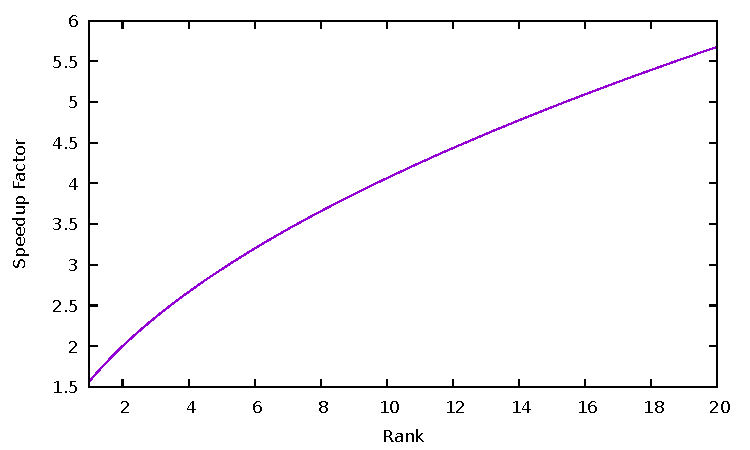
\includegraphics[width=11cm]{sum-speedup.pdf}
    \caption{Graph of exponential sum speedup factor. }
    \label{fig:sum-speedup}
 
    (Plotted continuously with the $\Gamma$ function.)
\end{figure}

\section{Signed Permutation Templates}

The exponential sum seems less useful as it only
partitions the bands into $2$ buckets.
But both methods can be combined with improved results.
Define a homomorphism $\psi \colon B_{n} \rightarrow S_{n} \times \Z$
by $\psi(x) = (\phi(x), \gamma(x))$.
The $k$-templates for $\psi$ are tuples
of signed transpositions.
This set $T_{k}$ is the Cartesian product of the permutation
templates and the exponential sum templates.

\begin{proposition}
The speedup factor for using signed permutation templates is just the product of each
separate method's speedup factor:
\[
    \frac{2^{k} {n \choose 2}}{ { k \choose \floor{\frac{k + 1}{2}}}}.
\]
\end{proposition}

Trying out our original test values $n = 3$ and $k = 3$,
and assuming $p$ is the worst case $\floor{\frac{k + 1}{2}}$, we improve
the runtime from naive search by a factor of $8$.

\begin{figure}[h]
    \centering
    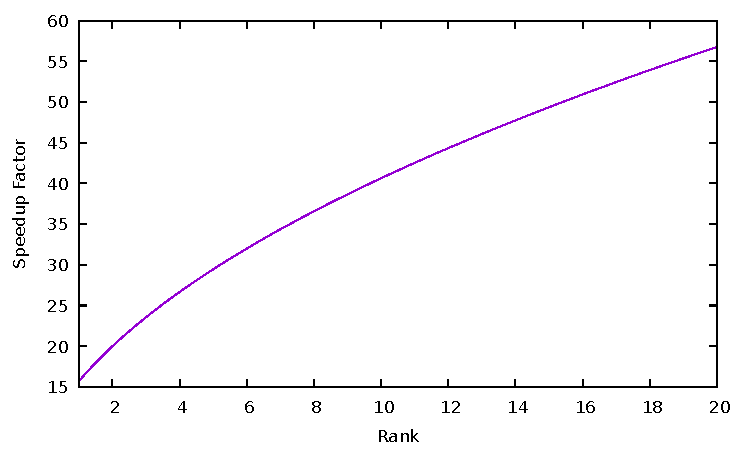
\includegraphics[width=11cm]{combined-speedup.pdf}

    \caption{Graph of signed permutation speedup factor for $n = 5$ strands.}
    \label{fig:combined-speedup}

    (Plotted continuously with the $\Gamma$ function.)
\end{figure}

\section{Implementation Notes}

Several steps of Algorithm \ref{alg:templated-search} describe how to generate sets. 
Sometimes these sets are very large and care should be
taken to enumerate them one at a time, rather then generating them all at once.
In our implementation we chose to 
generate all the templates and bands beforehand,
and then to only enumerate the various band presentations.

\subsection{Parallelization/Threading}

Sorting and merging to remove duplicates from each band
bucket can be done in parallel.

Each band presentation comparison with the braid word
can be considered independently.
However, iterating them independently is probably not convenient.
A more natural way to divide the work is to process
each template in parallel.

\subsection{GPU computing}

We also considered whether computations using a GPU would make sense,
as the band presentation search resembles hash/nonce searches used to crack cryptography.
We wrote a word problem implementation ideal for a GPU.
However, after further analysis realized the templated search wouldn't do well. 
The issue is sharing the buckets of bands with the various compute units.
Each GPU compute unit has a tiny memory cache.
The words from the buckets must be pulled into the cache in order to do their word problem check.
Thus, a lot of the time would be spent waiting for data to arrive, instead of 
performing computations

\section{Example of Computation}

Recall the braid which our upper bound algorithm
could not solve: $x = \inv{2} \inv{2} 1 \inv{2} 1$ (see example \ref{ex:does-not-solve}).
Using our bounding methods we conclude that $1 \leq rk(x) \leq 5$.
We suspect there is a band presentation of $3$ bands having maximum conjugate length $l \leq 3$.
There are $1029$  distinct bands in the $3$ strand braid group with this maximum conjugate length.
Therefore the naive search (after removing duplicates)
would compare $1029^{3} = 1,089,547,389$ band presentations.

The signed permutation buckets each have about 10 bands after removing duplicates:
\begin{itemize}
    \item $C_{(1 2)}$ has 9 bands.
    \item $C_{-(1 2)}$ has 9.
    \item $C_{(1 3)}$ has 10.
    \item \ldots
\end{itemize}

We enumerate each $3$-template for $x$.
There are 27 total:
\begin{itemize}
    \item $-(1 3), -(1 2), (1 2)$ has 810 presentations to check.
    \item $(1  2), -(1 3), -(2  3)$ has 810.
    \item \ldots
\end{itemize}
After checking all of these (fewer than $27,000$ total band presentations), we find $5$ band
presentations for $x$:
\[
\begin{split}
\inv{2}\inv{2}1\inv{2}\inv{1}22, 3\inv{1}2\inv{3}\inv{2}1\inv{3}, \inv{1}\inv{1}\inv{1}2111 \\
\inv{2}\inv{2}1\inv{2}\inv{1}22, \inv{2}\inv{2}1\inv{2}\inv{1}22, 3123\inv{2}\inv{1}\inv{3} \\
3\inv{1}2\inv{3}\inv{2}1\inv{3}, \inv{1}\inv{1}\inv{1}2111, 3\inv{1}2\inv{3}\inv{2}1\inv{3} \\
\inv{2}\inv{2}1\inv{2}\inv{1}22, 3123\inv{2}\inv{1}\inv{3}, 3\inv{1}2\inv{3}\inv{2}1\inv{3} \\
3123\inv{2}\inv{1}\inv{3}, 3\inv{1}2\inv{3}\inv{2}1\inv{3}, 3\inv{1}2\inv{3}\inv{2}1\inv{3}. \\
\end{split}
\]

%%%%%%%%%%%%%%%%%%%%%%%%%%%%%%%%%%%%%%%%%%%%%%%%%%%%%%%%%%%%%%%%%%%%%%%%%%%%%%%%%%%%%%%%%%
%% \appendix changes the numbering of chapters and sections for appendices. Any chapters or 
%% sections listed here will be treated as part of the appendix
\appendix

\chapter{Implementations of Selected Algorithms in Common Lisp}

The full source code for a program
that computes bounds on braid rank,
as well as a program for brute force searching with the template method,
can be found at the GitHub page: \url{https://github.com/justinmeiners/braid-rank-thesis}.

This appendix includes a selection of generally useful algorithms
that are self contained and concise.

\section{Rank in the Free Group}

\label{free-rank-code}

\begin{singlespace}
    \lstinputlisting[language=Lisp]{code/free-rank.lisp}
\end{singlespace}

\section{Rank Upper Bound in the Braid Group}

The \textbf{identity-p} function used in this sample
is not included.
This function is an implementation of one of the word problem solutions
discussed in Chapter \ref{chap:word-problem}.
Several implementations can be found on the GitHub page.

\label{braid-rank-code}

\begin{singlespace}
    \lstinputlisting[language=Lisp]{code/braid-rank.lisp}
\end{singlespace}

\chapter{Table of Computed Knot Results}

\label{knotinfo-table} 

The following table lists knots from the KnotInfo 
database \cite{knotinfo},
for which our rank method proved interesting properties.
The properties listed are the following:
\begin{itemize}
    \item P: The knot is quasipositive. This is shown when the exponential sum $\gamma$ is equal to computed rank $rk$.
    \item N: The knot is quasinegative. The exponential sum is equal to the negation of the computed rank.
    \item R: The knot has equal slice and ribbon genus.
        The $l$ column is the lower bound on the rank
        genus predicted by the slice genus $g_{s}$ and the number of strands $n$:
        \[
            l = 2g_{s} - 1 + n \leq rk
        \].
        When $rk = 2g_{s} - 1$ then it's know that the slice genus
        and the ribbon genus of the corresponding knots are equal
        (see the discussion for (\ref{eq:rank-and-ribbon-genus})).

   \item *: According to KnotInfo, showing this knot is quasipositive or
            quasinegative requires
            advanced techniques.
            Our method may offer a simpler alternative.
\end{itemize}

\small
\begin{singlespace}

\begin{center}
\begin{longtable}{ | l | l | c | c | c | c | c | l |}
    \hline
    Name & Chosen Braid & n & $g_{s}$ & l & $\gamma$ & $rk$ & Properties \\
    \hline 
    3 1 & $111$ & 2 & 1 & 3 & 3 & 3 & R P \\
4 1 & $1\inv{2}1\inv{2}$ & 3 & 1 & 4 & 0 & 4 & R \\
5 1 & $11111$ & 2 & 2 & 5 & 5 & 5 & R P \\
5 2 & $1112\inv{1}2$ & 3 & 1 & 4 & 4 & 4 & R P \\
7 1 & $1111111$ & 2 & 3 & 7 & 7 & 7 & R P \\
7 2 & $1112\inv{1}23\inv{2}3$ & 4 & 1 & 5 & 5 & 5 & R P \\
7 3 & $111112\inv{1}2$ & 3 & 2 & 6 & 6 & 6 & R P \\
7 4 & $112\inv{1}223\inv{2}3$ & 4 & 1 & 5 & 5 & 5 & R P \\
7 5 & $11112\inv{1}22$ & 3 & 2 & 6 & 6 & 6 & R P \\
8 1 & $112\inv{1}23\inv{2}\inv{4}3\inv{4}$ & 5 & 1 & 6 & 2 & 6 & R \\
8 3 & $112\inv{1}\inv{3}2\inv{3}\inv{4}3\inv{4}$ & 5 & 1 & 6 & 0 & 6 & R \\
8 15 & $11\inv{2}132223$ & 4 & 2 & 7 & 7 & 7 & R P \\
8 19 & $11121112$ & 3 & 3 & 8 & 8 & 8 & R P \\
8 20 & $111\inv{2}\inv{1}\inv{1}\inv{1}\inv{2}$ & 3 & 0 & 2 & -2 & 2 & R N * \\
8 21 & $1112\inv{1}\inv{1}22$ & 3 & 1 & 4 & 4 & 4 & R P * \\
9 1 & $111111111$ & 2 & 4 & 9 & 9 & 9 & R P \\
9 2 & $1112\inv{1}23\inv{2}34\inv{3}4$ & 5 & 1 & 6 & 6 & 6 & R P \\
9 3 & $11111112\inv{1}2$ & 3 & 3 & 8 & 8 & 8 & R P \\
9 4 & $111112\inv{1}23\inv{2}3$ & 4 & 2 & 7 & 7 & 7 & R P \\
9 5 & $112\inv{1}223\inv{2}34\inv{3}4$ & 5 & 1 & 6 & 6 & 6 & R P \\
9 6 & $1111112\inv{1}22$ & 3 & 3 & 8 & 8 & 8 & R P \\
9 7 & $11112\inv{1}23\inv{2}33$ & 4 & 2 & 7 & 7 & 7 & R P \\
9 9 & $111112\inv{1}222$ & 3 & 3 & 8 & 8 & 8 & R P \\
9 10 & $112\inv{1}22223\inv{2}3$ & 4 & 2 & 7 & 7 & 7 & R P \\
9 13 & $11112\inv{1}223\inv{2}3$ & 4 & 2 & 7 & 7 & 7 & R P \\
9 16 & $111122\inv{1}222$ & 3 & 3 & 8 & 8 & 8 & R P \\
9 18 & $1112\inv{1}2223\inv{2}3$ & 4 & 2 & 7 & 7 & 7 & R P \\
9 23 & $1112\inv{1}223\inv{2}33$ & 4 & 2 & 7 & 7 & 7 & R P \\
9 35 & $112\inv{1}223\inv{2}\inv{2}4\inv{3}243$ & 5 & 1 & 6 & 6 & 6 & R P \\
9 42 & $\inv{1}\inv{1}\inv{1}211\inv{3}2\inv{3}$ & 4 & 1 & 5 & -1 & 5 & R \\
9 44 & $1112\inv{1}\inv{1}\inv{3}2\inv{3}$ & 4 & 1 & 5 & 1 & 5 & R \\
9 45 & $\inv{1}\inv{1}\inv{2}1\inv{2}\inv{1}\inv{3}2\inv{3}$ & 4 & 1 & 5 & -5 & 5 & R N * \\
9 46 & $\inv{1}2\inv{1}2\inv{3}\inv{2}1\inv{2}\inv{3}$ & 4 & 0 & 3 & -3 & 3 & R N \\
10 1 & $112\inv{1}23\inv{2}34\inv{3}\inv{5}4\inv{5}$ & 6 & 1 & 7 & 3 & 7 & R \\
10 49 & $1111\inv{2}132223$ & 4 & 3 & 9 & 9 & 9 & R P \\
10 53 & $112\inv{1}2\inv{3}243334$ & 5 & 2 & 8 & 8 & 8 & R P \\
10 55 & $1112\inv{1}\inv{3}243334$ & 5 & 2 & 8 & 8 & 8 & R P \\
10 63 & $11\inv{2}1322234\inv{3}4$ & 5 & 2 & 8 & 8 & 8 & R P \\
10 66 & $111\inv{2}1322233$ & 4 & 3 & 9 & 9 & 9 & R P \\
10 80 & $111\inv{2}1132223$ & 4 & 3 & 9 & 9 & 9 & R P \\
10 101 & $1112\inv{1}3\inv{2}13224\inv{3}4$ & 5 & 2 & 8 & 8 & 8 & R P \\
10 120 & $112\inv{1}\inv{3}\inv{2}14322334$ & 5 & 2 & 8 & 8 & 8 & R P \\
10 124 & $1111121112$ & 3 & 4 & 10 & 10 & 10 & R P \\
10 125 & $\inv{1}\inv{1}\inv{1}\inv{1}\inv{1}21112$ & 3 & 1 & 4 & 0 & 4 & R \\
10 126 & $\inv{1}\inv{1}\inv{1}\inv{1}\inv{1}\inv{2}111\inv{2}$ & 3 & 1 & 4 & -4 & 4 & R N * \\
10 127 & $111112\inv{1}\inv{1}22$ & 3 & 2 & 6 & 6 & 6 & R P * \\
10 128 & $111211223\inv{2}3$ & 4 & 3 & 9 & 9 & 9 & R P \\
10 130 & $111\inv{2}\inv{1}\inv{1}\inv{2}\inv{2}\inv{3}2\inv{3}$ & 4 & 1 & 5 & -3 & 5 & R \\
10 131 & $1112\inv{1}\inv{1}223\inv{2}3$ & 4 & 1 & 5 & 5 & 5 & R P * \\
10 132 & $111\inv{2}\inv{1}\inv{1}\inv{2}\inv{3}2\inv{3}\inv{3}$ & 4 & 1 & 5 & -3 & 5 & R \\
10 133 & $1112\inv{1}\inv{1}23\inv{2}33$ & 4 & 1 & 5 & 5 & 5 & R P * \\
10 134 & $11121123\inv{2}33$ & 4 & 3 & 9 & 9 & 9 & R P \\
10 139 & $1111211122$ & 3 & 4 & 10 & 10 & 10 & R P \\
10 140 & $\inv{1}\inv{1}\inv{1}211123\inv{2}3$ & 4 & 0 & 3 & 3 & 3 & R P * \\
10 141 & $\inv{1}\inv{1}\inv{1}\inv{1}211122$ & 3 & 1 & 4 & 2 & 4 & R \\
10 142 & $111211123\inv{2}3$ & 4 & 3 & 9 & 9 & 9 & R P \\
10 143 & $\inv{1}\inv{1}\inv{1}\inv{1}\inv{2}111\inv{2}\inv{2}$ & 3 & 1 & 4 & -4 & 4 & R N * \\
10 145 & $\inv{1}\inv{1}\inv{2}1\inv{2}\inv{1}\inv{3}\inv{2}1\inv{2}\inv{3}$ & 4 & 2 & 7 & -7 & 7 & R N * \\
10 147 & $111\inv{2}1\inv{2}\inv{3}2\inv{1}2\inv{3}$ & 4 & 1 & 5 & 1 & 5 & R \\
10 148 & $\inv{1}\inv{1}\inv{1}\inv{1}\inv{2}11\inv{2}1\inv{2}$ & 3 & 1 & 4 & -4 & 4 & R N * \\
10 149 & $11112\inv{1}2\inv{1}22$ & 3 & 2 & 6 & 6 & 6 & R P \\
10 150 & $111\inv{2}113\inv{2}\inv{1}32$ & 4 & 2 & 7 & 5 & 7 & R \\
10 152 & $1112211222$ & 3 & 4 & 10 & 10 & 10 & R P \\
10 154 & $112\inv{1}2132223$ & 4 & 3 & 9 & 9 & 9 & R P \\
10 156 & $\inv{1}\inv{1}\inv{1}211\inv{3}\inv{2}1\inv{2}\inv{3}$ & 4 & 1 & 5 & -3 & 5 & R \\
10 157 & $\inv{1}\inv{1}\inv{1}\inv{2}\inv{2}1\inv{2}1\inv{2}\inv{2}$ & 3 & 2 & 6 & -6 & 6 & R N * \\
10 159 & $1112\inv{1}2\inv{1}\inv{1}22$ & 3 & 1 & 4 & 4 & 4 & R P * \\
10 161 & $1112\inv{1}21122$ & 3 & 3 & 8 & 8 & 8 & R P \\
10 164 & $11\inv{2}1\inv{2}\inv{2}\inv{3}2\inv{1}2\inv{3}$ & 4 & 1 & 5 & -1 & 5 & R \\
11a 43 & $112\inv{1}21\inv{3}2433344$ & 5 & 3 & 10 & 10 & 10 & R P \\
11a 94 & $111122\inv{1}223\inv{2}33$ & 4 & 3 & 9 & 9 & 9 & R P \\
11a 95 & $1112\inv{1}223\inv{2}34\inv{3}44$ & 5 & 2 & 8 & 8 & 8 & R P \\
11a 186 & $1112\inv{1}22223\inv{2}33$ & 4 & 3 & 9 & 9 & 9 & R P \\
11a 191 & $111112\inv{1}223\inv{2}33$ & 4 & 3 & 9 & 9 & 9 & R P \\
11a 192 & $1112\inv{1}223\inv{2}334\inv{3}4$ & 5 & 2 & 8 & 8 & 8 & R P \\
11a 200 & $1112\inv{1}223\inv{2}\inv{2}4\inv{3}2443$ & 5 & 2 & 8 & 8 & 8 & R P \\
11a 211 & $\inv{1}\inv{1}\inv{2}1\inv{2}\inv{3}2\inv{3}4\inv{3}\inv{5}4\inv{5}$ & 6 & 2 & 9 & -5 & 9 & R \\
11a 234 & $111111112\inv{1}22$ & 3 & 4 & 10 & 10 & 10 & R P \\
11a 235 & $1112\inv{1}222223\inv{2}3$ & 4 & 3 & 9 & 9 & 9 & R P \\
11a 236 & $11112\inv{1}2223\inv{2}33$ & 4 & 3 & 9 & 9 & 9 & R P \\
11a 237 & $1112\inv{1}2223\inv{2}\inv{2}4\inv{3}243$ & 5 & 2 & 8 & 8 & 8 & R P \\
11a 238 & $1112\inv{1}2223\inv{2}34\inv{3}4$ & 5 & 2 & 8 & 8 & 8 & R P \\
11a 240 & $11111122\inv{1}222$ & 3 & 4 & 10 & 10 & 10 & R P \\
11a 241 & $111122\inv{1}2223\inv{2}3$ & 4 & 3 & 9 & 9 & 9 & R P \\
11a 242 & $1111112\inv{1}23\inv{2}33$ & 4 & 3 & 9 & 9 & 9 & R P \\
11a 243 & $1112\inv{1}23\inv{2}3334\inv{3}4$ & 5 & 2 & 8 & 8 & 8 & R P \\
11a 245 & $11112\inv{1}233\inv{2}333$ & 4 & 3 & 9 & 9 & 9 & R P \\
11a 246 & $11112\inv{1}23\inv{2}34\inv{3}44$ & 5 & 2 & 8 & 8 & 8 & R P \\
11a 247 & $1112\inv{1}23\inv{2}34\inv{3}45\inv{4}5$ & 6 & 1 & 7 & 7 & 7 & R P \\
11a 263 & $111122\inv{1}322233$ & 4 & 4 & 11 & 11 & 11 & R P \\
11a 334 & $1111112\inv{1}2222$ & 3 & 4 & 10 & 10 & 10 & R P \\
11a 335 & $111112\inv{1}2223\inv{2}3$ & 4 & 3 & 9 & 9 & 9 & R P \\
11a 336 & $1111112\inv{1}223\inv{2}3$ & 4 & 3 & 9 & 9 & 9 & R P \\
11a 337 & $112\inv{1}2223\inv{2}334\inv{3}4$ & 5 & 2 & 8 & 8 & 8 & R P \\
11a 338 & $11111222\inv{1}222$ & 3 & 4 & 10 & 10 & 10 & R P \\
11a 339 & $111112\inv{1}23\inv{2}333$ & 4 & 3 & 9 & 9 & 9 & R P \\
11a 340 & $1111222\inv{1}223\inv{2}3$ & 4 & 3 & 9 & 9 & 9 & R P \\
11a 341 & $11112\inv{1}23\inv{2}334\inv{3}4$ & 5 & 2 & 8 & 8 & 8 & R P \\
11a 342 & $111112\inv{1}23\inv{2}34\inv{3}4$ & 5 & 2 & 8 & 8 & 8 & R P \\
11a 343 & $112\inv{1}223\inv{2}34\inv{3}45\inv{4}5$ & 6 & 1 & 7 & 7 & 7 & R P \\
11a 355 & $11111112\inv{1}222$ & 3 & 4 & 10 & 10 & 10 & R P \\
11a 356 & $11112\inv{1}22223\inv{2}3$ & 4 & 3 & 9 & 9 & 9 & R P \\
11a 357 & $11112\inv{1}223\inv{2}333$ & 4 & 3 & 9 & 9 & 9 & R P \\
11a 358 & $11111112\inv{1}23\inv{2}3$ & 4 & 3 & 9 & 9 & 9 & R P \\
11a 359 & $112\inv{1}22223\inv{2}34\inv{3}4$ & 5 & 2 & 8 & 8 & 8 & R P \\
11a 360 & $11112\inv{1}223\inv{2}34\inv{3}4$ & 5 & 2 & 8 & 8 & 8 & R P \\
11a 361 & $11112\inv{1}223\inv{2}\inv{2}4\inv{3}243$ & 5 & 2 & 8 & 8 & 8 & R P \\
11a 362 & $112\inv{1}223\inv{2}\inv{2}4\inv{3}245\inv{4}35$ & 6 & 1 & 7 & 7 & 7 & R P \\
11a 363 & $112\inv{1}23\inv{2}334\inv{3}45\inv{4}5$ & 6 & 1 & 7 & 7 & 7 & R P \\
11a 364 & $1111111112\inv{1}2$ & 3 & 4 & 10 & 10 & 10 & R P \\
11a 365 & $112\inv{1}2222223\inv{2}3$ & 4 & 3 & 9 & 9 & 9 & R P \\
11a 366 & $112\inv{1}22223\inv{2}\inv{2}4\inv{3}243$ & 5 & 2 & 8 & 8 & 8 & R P \\
11a 367 & $11111111111$ & 2 & 5 & 11 & 11 & 11 & R P \\
11n 1 & $\inv{1}\inv{1}\inv{1}\inv{2}1\inv{3}2\inv{3}\inv{2}\inv{4}3\inv{4}$ & 5 & 1 & 6 & -6 & 6 & R N \\
11n 10 & $\inv{1}\inv{1}\inv{1}\inv{2}1\inv{2}\inv{2}\inv{1}\inv{3}2\inv{3}$ & 4 & 2 & 7 & -7 & 7 & R N \\
11n 12 & $11\inv{2}1\inv{2}\inv{2}32\inv{1}23$ & 4 & 1 & 5 & 3 & 5 & R \\
11n 14 & $\inv{1}\inv{1}\inv{1}\inv{1}\inv{2}1\inv{2}\inv{1}\inv{3}2\inv{3}$ & 4 & 2 & 7 & -7 & 7 & R N \\
11n 17 & $\inv{1}\inv{1}\inv{2}1\inv{2}\inv{3}2\inv{3}\inv{2}\inv{4}3\inv{4}$ & 5 & 1 & 6 & -6 & 6 & R N \\
11n 18 & $112\inv{1}223\inv{2}\inv{2}\inv{4}3\inv{4}$ & 5 & 1 & 6 & 2 & 6 & R \\
11n 19 & $\inv{1}\inv{1}\inv{1}\inv{1}\inv{1}211\inv{3}2\inv{3}$ & 4 & 2 & 7 & -3 & 7 & R \\
11n 20 & $\inv{1}\inv{1}\inv{2}1\inv{2}\inv{2}322\inv{4}3\inv{4}$ & 5 & 1 & 6 & -2 & 6 & R \\
11n 28 & $1112\inv{1}\inv{1}23\inv{2}\inv{4}3\inv{4}$ & 5 & 1 & 6 & 2 & 6 & R \\
11n 35 & $11\inv{2}1\inv{2}132233$ & 4 & 2 & 7 & 7 & 7 & R P \\
11n 38 & $111\inv{2}\inv{1}\inv{3}2\inv{1}2\inv{3}\inv{2}$ & 4 & 1 & 5 & -1 & 5 & R \\
11n 40 & $1\inv{2}1\inv{2}\inv{2}132223$ & 4 & 1 & 5 & 5 & 5 & R P \\
11n 43 & $11\inv{2}1\inv{2}132223$ & 4 & 2 & 7 & 7 & 7 & R P \\
11n 48 & $\inv{1}\inv{1}\inv{1}\inv{1}\inv{2}1113\inv{2}3$ & 4 & 1 & 5 & -1 & 5 & R \\
11n 51 & $\inv{1}\inv{1}\inv{1}2113\inv{2}132$ & 4 & 1 & 5 & 3 & 5 & R \\
11n 54 & $112\inv{1}\inv{1}213\inv{2}33$ & 4 & 1 & 5 & 5 & 5 & R P \\
11n 59 & $111\inv{2}1\inv{2}32223$ & 4 & 2 & 7 & 7 & 7 & R P \\
11n 62 & $1112\inv{1}\inv{1}\inv{3}2\inv{3}\inv{4}3\inv{4}$ & 5 & 1 & 6 & 0 & 6 & R \\
11n 63 & $112\inv{1}213\inv{2}34\inv{3}4$ & 5 & 1 & 6 & 6 & 6 & R P \\
11n 65 & $\inv{1}\inv{2}1\inv{2}\inv{2}\inv{3}2\inv{1}22\inv{3}$ & 4 & 1 & 5 & -3 & 5 & R \\
11n 72 & $11\inv{2}\inv{2}1322233$ & 4 & 2 & 7 & 7 & 7 & R P \\
11n 75 & $\inv{1}\inv{1}222\inv{1}\inv{3}\inv{2}\inv{2}\inv{2}\inv{3}$ & 4 & 1 & 5 & -5 & 5 & R N \\
11n 77 & $11221322233$ & 4 & 4 & 11 & 11 & 11 & R P \\
11n 79 & $111\inv{2}\inv{1}\inv{1}3\inv{2}34\inv{3}4$ & 5 & 1 & 6 & 2 & 6 & R \\
11n 82 & $1111\inv{2}\inv{1}\inv{1}\inv{1}3\inv{2}3$ & 4 & 1 & 5 & 1 & 5 & R \\
11n 84 & $\inv{1}\inv{1}2\inv{1}2\inv{3}\inv{2}1\inv{2}\inv{2}\inv{3}$ & 4 & 1 & 5 & -5 & 5 & R N \\
11n 85 & $\inv{1}\inv{1}\inv{1}21112\inv{3}2\inv{3}$ & 4 & 1 & 5 & 1 & 5 & R \\
11n 87 & $\inv{1}\inv{1}\inv{2}1\inv{2}\inv{1}\inv{3}2\inv{1}\inv{3}2$ & 4 & 1 & 5 & -5 & 5 & R N \\
11n 89 & $\inv{1}\inv{1}\inv{1}2\inv{1}\inv{3}\inv{2}1\inv{2}\inv{2}\inv{3}$ & 4 & 2 & 7 & -7 & 7 & R N \\
11n 91 & $\inv{1}\inv{1}\inv{2}13\inv{2}\inv{4}\inv{3}2\inv{3}\inv{3}\inv{4}$ & 5 & 1 & 6 & -6 & 6 & R N \\
11n 95 & $1112\inv{1}232\inv{1}23$ & 4 & 2 & 7 & 7 & 7 & R P \\
11n 99 & $\inv{1}\inv{2}1\inv{2}\inv{2}\inv{2}\inv{3}2\inv{1}2\inv{3}$ & 4 & 1 & 5 & -5 & 5 & R N \\
11n 105 & $11\inv{2}1\inv{2}322233$ & 4 & 2 & 7 & 7 & 7 & R P \\
11n 106 & $\inv{1}\inv{1}\inv{1}2111\inv{3}2\inv{3}\inv{3}$ & 4 & 1 & 5 & -1 & 5 & R \\
11n 108 & $\inv{1}\inv{1}2\inv{1}\inv{1}\inv{3}\inv{2}1\inv{2}\inv{2}\inv{3}$ & 4 & 2 & 7 & -7 & 7 & R N \\
11n 109 & $\inv{1}\inv{1}\inv{1}2\inv{1}\inv{1}\inv{3}\inv{2}1\inv{2}\inv{3}$ & 4 & 2 & 7 & -7 & 7 & R N \\
11n 110 & $1112\inv{1}\inv{1}\inv{3}2\inv{1}2\inv{3}$ & 4 & 1 & 5 & 1 & 5 & R \\
11n 113 & $\inv{1}\inv{1}\inv{2}13\inv{2}\inv{2}\inv{4}\inv{3}2\inv{3}\inv{4}$ & 5 & 1 & 6 & -6 & 6 & R N \\
11n 118 & $111213\inv{2}1\inv{2}32$ & 4 & 2 & 7 & 7 & 7 & R P \\
11n 122 & $\inv{1}\inv{1}\inv{1}2\inv{1}2\inv{3}\inv{2}1\inv{2}\inv{3}$ & 4 & 1 & 5 & -5 & 5 & R N \\
11n 127 & $\inv{1}\inv{1}\inv{2}11\inv{2}\inv{2}\inv{1}\inv{3}2\inv{3}$ & 4 & 1 & 5 & -5 & 5 & R N \\
11n 134 & $\inv{1}\inv{1}\inv{2}1\inv{2}\inv{2}\inv{3}2\inv{1}2\inv{3}$ & 4 & 1 & 5 & -5 & 5 & R N \\
11n 136 & $1112\inv{1}3\inv{2}113222$ & 4 & 3 & 9 & 9 & 9 & R P \\
11n 138 & $\inv{1}\inv{2}1\inv{2}\inv{3}2\inv{1}222\inv{3}$ & 4 & 1 & 5 & -1 & 5 & R \\
11n 139 & $112\inv{1}3\inv{2}34\inv{3}2\inv{3}4$ & 5 & 0 & 4 & 4 & 4 & R P \\
11n 142 & $112\inv{1}\inv{3}\inv{2}\inv{4}3\inv{2}3\inv{4}\inv{3}$ & 5 & 1 & 6 & -2 & 6 & R \\
11n 143 & $11\inv{2}1\inv{2}1\inv{3}2\inv{1}2\inv{3}$ & 4 & 1 & 5 & 1 & 5 & R \\
11n 144 & $11\inv{2}1132\inv{1}233$ & 4 & 2 & 7 & 7 & 7 & R P \\
11n 162 & $112\inv{1}213\inv{2}\inv{1}324\inv{3}4$ & 5 & 1 & 6 & 6 & 6 & R P \\
11n 174 & $11\inv{2}13\inv{2}13223$ & 4 & 2 & 7 & 7 & 7 & R P \\
11n 176 & $\inv{1}\inv{1}2\inv{1}2\inv{1}\inv{3}\inv{2}1\inv{2}\inv{3}$ & 4 & 1 & 5 & -5 & 5 & R N \\
11n 180 & $11112\inv{1}3\inv{2}11322$ & 4 & 3 & 9 & 9 & 9 & R P \\
11n 183 & $1\inv{2}132213223$ & 4 & 3 & 9 & 9 & 9 & R P \\
11n 185 & $1\inv{2}13\inv{2}132223$ & 4 & 2 & 7 & 7 & 7 & R P \\
12a 43 & $\inv{1}223134122\inv{3}244$ & 5 & 3 & 10 & 10 & 10 & R P \\
12a 52 & $1223131111\inv{2}31$ & 4 & 4 & 11 & 11 & 11 & R P \\
12a 53 & $122313134\inv{3}\inv{2}433$ & 5 & 3 & 10 & 10 & 10 & R P \\
12a 55 & $122341414\inv{3}\inv{2}433$ & 5 & 3 & 10 & 10 & 10 & R P \\
12a 56 & $1\inv{2}1234453\inv{4}252\inv{3}5$ & 6 & 2 & 9 & 9 & 9 & R P \\
12a 82 & $\inv{1}221123342\inv{3}244$ & 5 & 3 & 10 & 10 & 10 & R P \\
12a 93 & $1112231311\inv{2}31$ & 4 & 4 & 11 & 11 & 11 & R P \\
12a 94 & $12231313\inv{2}34\inv{3}43$ & 5 & 3 & 10 & 10 & 10 & R P \\
12a 96 & $12234\inv{3}141\inv{2}3333$ & 5 & 3 & 10 & 10 & 10 & R P \\
12a 97 & $123445352\inv{4}5\inv{3}21\inv{2}$ & 6 & 2 & 9 & 9 & 9 & R P \\
12a 143 & $1111122313\inv{2}31$ & 4 & 4 & 11 & 11 & 11 & R P \\
12a 144 & $122311\inv{2}3334\inv{3}43$ & 5 & 3 & 10 & 10 & 10 & R P \\
12a 145 & $122311\inv{2}3444\inv{3}43$ & 5 & 3 & 10 & 10 & 10 & R P \\
12a 152 & $12344535\inv{4}5321\inv{2}\inv{3}$ & 6 & 2 & 9 & 9 & 9 & R P \\
12a 255 & $\inv{1}234554\inv{5}43\inv{4}2\inv{1}2\inv{3}$ & 6 & 2 & 9 & 5 & 9 & R \\
12a 270 & $1\inv{2}123\inv{4}3\inv{4}54\inv{3}43\inv{5}22\inv{3}$ & 6 & 1 & 7 & 5 & 7 & R \\
12a 276 & $1222231311\inv{2}31$ & 4 & 4 & 11 & 11 & 11 & R P \\
12a 277 & $1\inv{2}123333422\inv{3}44$ & 5 & 3 & 10 & 10 & 10 & R P \\
12a 293 & $\inv{1}22313\inv{4}12223\inv{2}344$ & 5 & 3 & 10 & 10 & 10 & R P \\
12a 295 & $\inv{1}22112\inv{3}4243334$ & 5 & 3 & 10 & 10 & 10 & R P \\
12a 319 & $\inv{1}2231312\inv{3}4222\inv{3}43$ & 5 & 3 & 10 & 10 & 10 & R P \\
12a 320 & $112\inv{1}23\inv{2}\inv{4}\inv{3}25433345$ & 6 & 2 & 9 & 9 & 9 & R P \\
12a 344 & $1\inv{2}123342424\inv{3}44$ & 5 & 3 & 10 & 10 & 10 & R P \\
12a 345 & $1\inv{2}123345\inv{4}252\inv{3}44$ & 6 & 2 & 9 & 9 & 9 & R P \\
12a 355 & $1\inv{2}3133424\inv{3}2444$ & 5 & 3 & 10 & 10 & 10 & R P \\
12a 356 & $1\inv{2}12\inv{3}4522333\inv{4}54$ & 6 & 2 & 9 & 9 & 9 & R P \\
12a 367 & $1112222313\inv{2}31$ & 4 & 4 & 11 & 11 & 11 & R P \\
12a 368 & $12222311\inv{2}34\inv{3}43$ & 5 & 3 & 10 & 10 & 10 & R P \\
12a 386 & $\inv{1}2\inv{1}2\inv{3}\inv{3}\inv{4}\inv{2}\inv{2}3\inv{2}\inv{4}\inv{2}3$ & 5 & 2 & 8 & -6 & 8 & R \\
12a 391 & $\inv{1}223131332\inv{3}42\inv{3}43$ & 5 & 3 & 10 & 10 & 10 & R P \\
12a 392 & $112\inv{1}23\inv{2}\inv{4}\inv{3}25433455$ & 6 & 2 & 9 & 9 & 9 & R P \\
12a 420 & $1\inv{2}1233422\inv{3}4444$ & 5 & 3 & 10 & 10 & 10 & R P \\
12a 421 & $1\inv{2}1233422\inv{3}45\inv{4}54$ & 6 & 2 & 9 & 9 & 9 & R P \\
12a 432 & $\inv{1}223131\inv{2}34222\inv{3}43$ & 5 & 3 & 10 & 10 & 10 & R P \\
12a 442 & $1\inv{2}341122222\inv{3}43$ & 5 & 3 & 10 & 10 & 10 & R P \\
12a 444 & $1\inv{2}3\inv{4}51\inv{3}524\inv{3}2445$ & 6 & 2 & 9 & 7 & 9 & R \\
12a 542 & $\inv{1}2\inv{1}23\inv{2}34\inv{3}4\inv{5}4\inv{3}4352$ & 6 & 2 & 9 & 5 & 9 & R \\
12a 556 & $\inv{1}221123\inv{2}34\inv{3}222\inv{3}\inv{4}$ & 5 & 2 & 8 & 6 & 8 & R \\
12a 563 & $\inv{1}2222112\inv{3}2\inv{3}43\inv{2}3\inv{4}$ & 5 & 2 & 8 & 6 & 8 & R \\
12a 564 & $1\inv{2}12\inv{3}23\inv{4}3\inv{4}54\inv{3}43\inv{5}2$ & 6 & 1 & 7 & 5 & 7 & R \\
12a 568 & $\inv{1}221123\inv{2}3334\inv{3}2\inv{3}\inv{4}$ & 5 & 2 & 8 & 6 & 8 & R \\
12a 574 & $1222222313\inv{2}31$ & 4 & 4 & 11 & 11 & 11 & R P \\
12a 575 & $1\inv{2}311222334\inv{3}43$ & 5 & 3 & 10 & 10 & 10 & R P \\
12a 586 & $\inv{1}223131222\inv{3}42\inv{3}43$ & 5 & 3 & 10 & 10 & 10 & R P \\
12a 610 & $1112\inv{1}3\inv{2}13224\inv{3}45\inv{4}5$ & 6 & 2 & 9 & 9 & 9 & R P \\
12a 615 & $\inv{1}22313122\inv{3}42433\inv{4}$ & 5 & 3 & 10 & 10 & 10 & R P \\
12a 623 & $\inv{1}22112\inv{3}2\inv{3}4443\inv{2}3\inv{4}$ & 5 & 2 & 8 & 6 & 8 & R \\
12a 638 & $\inv{1}22\inv{3}223131\inv{2}34\inv{3}\inv{2}4$ & 5 & 2 & 8 & 6 & 8 & R \\
12a 647 & $112223111\inv{2}133$ & 4 & 4 & 11 & 11 & 11 & R P \\
12a 648 & $1\inv{2}313342422\inv{3}24$ & 5 & 3 & 10 & 10 & 10 & R P \\
12a 653 & $1112\inv{1}23\inv{2}4\inv{3}24335\inv{4}5$ & 6 & 2 & 9 & 9 & 9 & R P \\
12a 677 & $\inv{1}22112\inv{3}4\inv{3}2\inv{3}\inv{2}3\inv{4}34$ & 5 & 1 & 6 & 4 & 6 & R \\
12a 679 & $123\inv{4}5352414\inv{2}45\inv{3}$ & 6 & 2 & 9 & 9 & 9 & R P \\
12a 685 & $\inv{1}221123\inv{2}344\inv{3}22\inv{3}\inv{4}$ & 5 & 2 & 8 & 6 & 8 & R \\
12a 735 & $1\inv{2}123\inv{2}3\inv{4}3\inv{4}54\inv{3}43\inv{5}2$ & 6 & 1 & 7 & 5 & 7 & R \\
12a 750 & $1223\inv{2}\inv{1}3\inv{4}3\inv{4}54\inv{3}4\inv{2}\inv{5}322$ & 6 & 1 & 7 & 5 & 7 & R \\
12a 787 & $1\inv{2}12\inv{3}\inv{4}3\inv{4}5\inv{4}3\inv{4}\inv{3}\inv{5}22\inv{3}$ & 6 & 2 & 9 & -1 & 9 & R \\
12a 803 & $1\inv{2}3\inv{4}5\inv{6}135\inv{6}24\inv{5}4\inv{3}2$ & 7 & 1 & 8 & 4 & 8 & R \\
12a 811 & $12231311\inv{2}3133$ & 4 & 4 & 11 & 11 & 11 & R P \\
12a 813 & $11122313\inv{2}3133$ & 4 & 4 & 11 & 11 & 11 & R P \\
12a 817 & $11223131\inv{2}3133$ & 4 & 4 & 11 & 11 & 11 & R P \\
12a 876 & $1112231333\inv{2}31$ & 4 & 4 & 11 & 11 & 11 & R P \\
12a 877 & $\inv{1}23342\inv{3}1412444$ & 5 & 3 & 10 & 10 & 10 & R P \\
12a 900 & $\inv{1}22\inv{3}42231312\inv{3}234$ & 5 & 3 & 10 & 10 & 10 & R P \\
12a 908 & $1\inv{2}12\inv{3}4\inv{3}223\inv{4}3\inv{4}22\inv{3}$ & 5 & 2 & 8 & 4 & 8 & R \\
12a 938 & $\inv{1}2\inv{3}\inv{2}3\inv{2}3131334\inv{3}24$ & 5 & 2 & 8 & 6 & 8 & R \\
12a 953 & $\inv{1}\inv{2}33\inv{2}112\inv{3}2334\inv{3}43$ & 5 & 2 & 8 & 6 & 8 & R \\
12a 973 & $1\inv{2}31223\inv{4}3\inv{2}324444$ & 5 & 3 & 10 & 10 & 10 & R P \\
12a 995 & $1\inv{2}3122223\inv{4}3\inv{2}3244$ & 5 & 3 & 10 & 10 & 10 & R P \\
12a 996 & $112\inv{1}23\inv{2}\inv{4}\inv{3}25433445$ & 6 & 2 & 9 & 9 & 9 & R P \\
12a 1004 & $1\inv{2}313424243\inv{2}32\inv{4}3$ & 5 & 3 & 10 & 10 & 10 & R P \\
12a 1035 & $\inv{1}2\inv{3}42311223333\inv{2}4$ & 5 & 3 & 10 & 10 & 10 & R P \\
12a 1037 & $112\inv{1}223\inv{2}4\inv{3}24335\inv{4}5$ & 6 & 2 & 9 & 9 & 9 & R P \\
12a 1097 & $112\inv{1}2\inv{3}\inv{2}14\inv{3}4322345\inv{4}5$ & 6 & 2 & 9 & 9 & 9 & R P \\
12a 1112 & $\inv{1}2\inv{3}423131332\inv{3}234$ & 5 & 3 & 10 & 10 & 10 & R P \\
12a 1166 & $1\inv{2}3\inv{4}\inv{5}\inv{6}135\inv{6}24\inv{5}4\inv{3}2$ & 7 & 1 & 8 & 2 & 8 & R \\
12a 1185 & $1\inv{2}\inv{3}41\inv{3}4223\inv{4}3\inv{2}\inv{3}24$ & 5 & 2 & 8 & 4 & 8 & R \\
12a 1287 & $\inv{1}2\inv{3}456\inv{1}\inv{3}\inv{5}6\inv{2}\inv{4}543\inv{2}$ & 7 & 1 & 8 & 0 & 8 & R \\
12n 5 & $\inv{1}2\inv{1}23\inv{4}\inv{3}4\inv{3}\inv{4}\inv{2}\inv{4}\inv{2}\inv{3}$ & 5 & 1 & 6 & -6 & 6 & R N \\
12n 13 & $\inv{1}2\inv{1}2\inv{3}\inv{4}53\inv{4}\inv{2}5\inv{2}\inv{3}$ & 6 & 1 & 7 & -3 & 7 & R \\
12n 25 & $\inv{1}23\inv{4}\inv{1}\inv{2}34\inv{3}2\inv{3}4$ & 5 & 1 & 6 & 0 & 6 & R \\
12n 46 & $\inv{1}23\inv{1}\inv{2}3245\inv{3}\inv{4}54$ & 6 & 1 & 7 & 3 & 7 & R \\
12n 53 & $\inv{1}2\inv{1}2\inv{3}433\inv{2}\inv{2}\inv{3}433$ & 5 & 1 & 6 & 2 & 6 & R \\
12n 54 & $\inv{1}2\inv{3}\inv{3}\inv{2}1\inv{2}\inv{2}\inv{2}312\inv{1}$ & 4 & 2 & 7 & -3 & 7 & R \\
12n 58 & $\inv{1}2\inv{1}2\inv{3}\inv{4}\inv{4}\inv{3}\inv{2}\inv{2}\inv{3}4\inv{3}\inv{4}$ & 5 & 2 & 8 & -8 & 8 & R N \\
12n 74 & $11122\inv{1}2322133$ & 4 & 4 & 11 & 11 & 11 & R P \\
12n 77 & $1\inv{2}12343434242\inv{3}$ & 5 & 3 & 10 & 10 & 10 & R P \\
12n 79 & $1\inv{2}123\inv{4}3\inv{4}34242\inv{3}$ & 5 & 1 & 6 & 6 & 6 & R P \\
12n 89 & $1\inv{2}33221112\inv{3}\inv{2}1$ & 4 & 3 & 9 & 7 & 9 & R \\
12n 91 & $122111\inv{2}322133$ & 4 & 4 & 11 & 11 & 11 & R P \\
12n 93 & $12231341\inv{2}\inv{2}\inv{3}244$ & 5 & 3 & 10 & 8 & 10 & R \\
12n 96 & $1\inv{2}12334242334\inv{3}$ & 5 & 3 & 10 & 10 & 10 & R P \\
12n 97 & $\inv{1}2\inv{3}\inv{1}\inv{3}2\inv{3}\inv{4}333\inv{4}$ & 5 & 1 & 6 & -2 & 6 & R \\
12n 103 & $122223131\inv{2}1\inv{2}\inv{3}$ & 4 & 3 & 9 & 7 & 9 & R \\
12n 105 & $111221\inv{2}322133$ & 4 & 4 & 11 & 11 & 11 & R P \\
12n 110 & $12234\inv{3}1431223\inv{2}$ & 5 & 3 & 10 & 10 & 10 & R P \\
12n 113 & $\inv{1}2\inv{1}2\inv{1}\inv{2}1\inv{2}\inv{2}\inv{2}\inv{2}\inv{2}$ & 3 & 2 & 6 & -6 & 6 & R N * \\
12n 114 & $11122\inv{1}\inv{1}22222$ & 3 & 3 & 8 & 8 & 8 & R P * \\
12n 117 & $1\inv{2}1222\inv{3}\inv{3}22333$ & 4 & 2 & 7 & 7 & 7 & R P \\
12n 120 & $\inv{1}\inv{1}223\inv{1}\inv{2}\inv{2}\inv{3}\inv{3}\inv{2}\inv{1}2$ & 4 & 2 & 7 & -5 & 7 & R \\
12n 121 & $\inv{1}\inv{2}11\inv{2}\inv{3}2\inv{1}\inv{2}\inv{2}\inv{3}\inv{3}2$ & 4 & 1 & 5 & -5 & 5 & R N \\
12n 123 & $1\inv{2}1\inv{2}3322\inv{3}43344$ & 5 & 2 & 8 & 8 & 8 & R P \\
12n 128 & $1\inv{2}1\inv{2}334242334\inv{3}$ & 5 & 2 & 8 & 8 & 8 & R P \\
12n 133 & $\inv{1}22112233\inv{2}1222\inv{3}$ & 4 & 3 & 9 & 9 & 9 & R P \\
12n 134 & $11223\inv{1}3\inv{1}\inv{2}3133$ & 4 & 3 & 9 & 7 & 9 & R \\
12n 136 & $112211\inv{2}322133$ & 4 & 4 & 11 & 11 & 11 & R P \\
12n 138 & $122\inv{3}411\inv{2}\inv{2}33244$ & 5 & 3 & 10 & 8 & 10 & R \\
12n 143 & $1\inv{2}\inv{3}412422\inv{3}\inv{2}4$ & 5 & 2 & 8 & 4 & 8 & R \\
12n 148 & $\inv{1}\inv{2}\inv{2}\inv{3}2\inv{1}\inv{2}\inv{2}\inv{2}\inv{2}\inv{3}\inv{3}2$ & 4 & 3 & 9 & -9 & 9 & R N \\
12n 149 & $\inv{1}2\inv{1}\inv{2}\inv{3}\inv{3}\inv{4}3\inv{2}\inv{3}\inv{3}\inv{2}\inv{4}3$ & 5 & 2 & 8 & -8 & 8 & R N \\
12n 153 & $1212\inv{3}22313212$ & 4 & 4 & 11 & 11 & 11 & R P \\
12n 154 & $\inv{1}21\inv{2}3\inv{2}\inv{2}\inv{3}1\inv{3}\inv{2}12$ & 4 & 1 & 5 & -1 & 5 & R \\
12n 155 & $122\inv{1}23\inv{2}\inv{2}33221$ & 4 & 2 & 7 & 7 & 7 & R P \\
12n 157 & $1\inv{2}34122\inv{3}423\inv{2}$ & 5 & 1 & 6 & 6 & 6 & R P \\
12n 159 & $\inv{1}\inv{2}1\inv{2}3\inv{2}\inv{2}\inv{3}1\inv{3}\inv{2}\inv{1}2$ & 4 & 1 & 5 & -5 & 5 & R N \\
12n 166 & $12222\inv{1}2322133$ & 4 & 4 & 11 & 11 & 11 & R P \\
12n 169 & $122112\inv{3}2334\inv{3}43$ & 5 & 3 & 10 & 10 & 10 & R P \\
12n 176 & $12211\inv{2}3\inv{2}34\inv{3}2\inv{3}4$ & 5 & 1 & 6 & 6 & 6 & R P \\
12n 177 & $1\inv{2}1234432233\inv{4}3$ & 5 & 3 & 10 & 10 & 10 & R P \\
12n 183 & $1\inv{2}341242\inv{3}423$ & 5 & 2 & 8 & 8 & 8 & R P \\
12n 185 & $11\inv{2}\inv{3}1223131\inv{2}1$ & 4 & 3 & 9 & 7 & 9 & R \\
12n 187 & $122221\inv{2}322133$ & 4 & 4 & 11 & 11 & 11 & R P \\
12n 190 & $1\inv{2}\inv{1}2\inv{1}\inv{1}\inv{1}\inv{2}1\inv{2}\inv{2}\inv{2}$ & 3 & 2 & 6 & -6 & 6 & R N * \\
12n 191 & $1112222\inv{1}\inv{1}222$ & 3 & 3 & 8 & 8 & 8 & R P \\
12n 194 & $111\inv{2}31312\inv{3}2\inv{1}2$ & 4 & 2 & 7 & 7 & 7 & R P \\
12n 199 & $\inv{1}2\inv{1}\inv{2}\inv{3}\inv{3}\inv{2}\inv{2}\inv{2}\inv{2}333$ & 4 & 2 & 7 & -5 & 7 & R \\
12n 200 & $1\inv{2}\inv{3}\inv{4}23\inv{4}\inv{3}\inv{2}3\inv{1}4\inv{1}\inv{2}$ & 5 & 1 & 6 & -4 & 6 & R \\
12n 203 & $12231312\inv{3}42\inv{3}43$ & 5 & 3 & 10 & 10 & 10 & R P \\
12n 211 & $1\inv{2}31\inv{2}34\inv{3}222\inv{3}\inv{2}\inv{4}$ & 5 & 1 & 6 & 2 & 6 & R \\
12n 215 & $\inv{1}223131\inv{2}34\inv{3}4\inv{2}3$ & 5 & 2 & 8 & 6 & 8 & R \\
12n 217 & $12211\inv{2}34222\inv{3}43$ & 5 & 3 & 10 & 10 & 10 & R P \\
12n 221 & $1\inv{2}31334\inv{2}\inv{3}\inv{3}\inv{3}4$ & 5 & 1 & 6 & 2 & 6 & R \\
12n 222 & $122313412\inv{3}24\inv{3}\inv{2}$ & 5 & 2 & 8 & 8 & 8 & R P \\
12n 224 & $1\inv{2}3133\inv{4}\inv{2}\inv{3}\inv{3}\inv{3}\inv{4}$ & 5 & 1 & 6 & -2 & 6 & R \\
12n 233 & $1\inv{2}\inv{1}2\inv{1}\inv{2}1\inv{2}\inv{2}\inv{2}\inv{2}\inv{2}$ & 3 & 2 & 6 & -6 & 6 & R N * \\
12n 234 & $1\inv{2}\inv{2}112222222$ & 3 & 3 & 8 & 8 & 8 & R P * \\
12n 237 & $1\inv{2}\inv{2}33222221\inv{2}3$ & 4 & 2 & 7 & 7 & 7 & R P \\
12n 240 & $111\inv{2}\inv{2}332221\inv{2}3$ & 4 & 2 & 7 & 7 & 7 & R P \\
12n 242 & $122112222222$ & 3 & 5 & 12 & 12 & 12 & R P \\
12n 243 & $12233222221\inv{2}3$ & 4 & 4 & 11 & 11 & 11 & R P \\
12n 244 & $11122332221\inv{2}3$ & 4 & 4 & 11 & 11 & 11 & R P \\
12n 245 & $\inv{1}2342\inv{3}43231312$ & 5 & 3 & 10 & 10 & 10 & R P \\
12n 248 & $1\inv{2}\inv{3}\inv{4}3\inv{4}\inv{3}424\inv{1}\inv{3}\inv{1}\inv{2}$ & 5 & 1 & 6 & -4 & 6 & R \\
12n 249 & $1\inv{2}\inv{2}1122234\inv{2}\inv{3}43$ & 5 & 1 & 6 & 6 & 6 & R P \\
12n 250 & $12211\inv{2}\inv{2}\inv{2}\inv{3}\inv{4}23\inv{4}\inv{3}$ & 5 & 1 & 6 & 0 & 6 & R \\
12n 251 & $1221122234\inv{2}\inv{3}43$ & 5 & 3 & 10 & 10 & 10 & R P \\
12n 254 & $122311\inv{2}\inv{2}3321\inv{2}$ & 4 & 2 & 7 & 7 & 7 & R P \\
12n 259 & $122233\inv{2}1222\inv{3}\inv{1}21$ & 4 & 3 & 9 & 9 & 9 & R P \\
12n 262 & $\inv{1}2\inv{1}\inv{2}\inv{3}\inv{3}2\inv{3}\inv{4}2333\inv{4}$ & 5 & 1 & 6 & -2 & 6 & R \\
12n 269 & $\inv{1}2\inv{1}23443\inv{2}\inv{2}\inv{3}4\inv{3}\inv{4}$ & 5 & 2 & 8 & 0 & 8 & R \\
12n 270 & $\inv{1}2\inv{1}23\inv{4}\inv{3}\inv{3}\inv{2}\inv{2}3\inv{4}\inv{3}\inv{3}$ & 5 & 1 & 6 & -6 & 6 & R N \\
12n 273 & $1\inv{2}1\inv{2}\inv{3}42222\inv{3}4$ & 5 & 2 & 8 & 4 & 8 & R \\
12n 275 & $1\inv{2}3\inv{4}1\inv{2}\inv{4}\inv{3}2\inv{3}\inv{4}3$ & 5 & 1 & 6 & -2 & 6 & R \\
12n 276 & $\inv{1}\inv{2}\inv{2}1\inv{2}\inv{2}\inv{3}\inv{1}\inv{3}\inv{2}1\inv{2}\inv{3}$ & 4 & 3 & 9 & -9 & 9 & R N \\
12n 282 & $\inv{1}2\inv{3}\inv{4}\inv{1}\inv{2}3\inv{2}3\inv{4}\inv{3}2$ & 5 & 1 & 6 & -4 & 6 & R \\
12n 286 & $\inv{1}2\inv{3}\inv{1}2\inv{3}43\inv{2}324$ & 5 & 1 & 6 & 2 & 6 & R \\
12n 289 & $1\inv{2}1233424233\inv{4}3$ & 5 & 3 & 10 & 10 & 10 & R P \\
12n 292 & $1221112\inv{3}22133$ & 4 & 4 & 11 & 11 & 11 & R P \\
12n 303 & $1\inv{2}12\inv{3}\inv{3}2233333$ & 4 & 2 & 7 & 7 & 7 & R P \\
12n 305 & $1\inv{2}12332233333$ & 4 & 4 & 11 & 11 & 11 & R P \\
12n 306 & $1\inv{2}12\inv{3}\inv{3}223334\inv{3}4$ & 5 & 1 & 6 & 6 & 6 & R P \\
12n 308 & $1\inv{2}1233223334\inv{3}4$ & 5 & 3 & 10 & 10 & 10 & R P \\
12n 310 & $1\inv{2}123322\inv{3}\inv{3}\inv{3}\inv{4}3\inv{4}$ & 5 & 1 & 6 & 2 & 6 & R \\
12n 316 & $1\inv{2}12\inv{3}22\inv{3}22333$ & 4 & 2 & 7 & 7 & 7 & R P \\
12n 320 & $1\inv{2}\inv{3}1\inv{3}22\inv{1}2\inv{3}\inv{2}1\inv{2}$ & 4 & 1 & 5 & -1 & 5 & R \\
12n 321 & $\inv{1}23132\inv{1}231\inv{2}12$ & 4 & 2 & 7 & 7 & 7 & R P \\
12n 322 & $1\inv{2}313\inv{4}\inv{2}\inv{3}24\inv{3}\inv{4}$ & 5 & 1 & 6 & 0 & 6 & R \\
12n 328 & $1231322\inv{1}23212$ & 4 & 4 & 11 & 11 & 11 & R P \\
12n 329 & $\inv{1}\inv{2}\inv{2}\inv{3}\inv{1}\inv{1}2\inv{1}\inv{2}\inv{2}\inv{3}\inv{3}2$ & 4 & 3 & 9 & -9 & 9 & R N \\
12n 331 & $\inv{1}\inv{2}\inv{2}\inv{1}\inv{1}\inv{2}\inv{3}2\inv{3}43\inv{2}34$ & 5 & 2 & 8 & -4 & 8 & R \\
12n 332 & $\inv{1}2\inv{1}\inv{2}3\inv{4}\inv{3}\inv{3}\inv{2}\inv{2}3\inv{4}\inv{3}\inv{3}$ & 5 & 2 & 8 & -8 & 8 & R N \\
12n 334 & $1\inv{2}\inv{2}\inv{1}\inv{1}\inv{2}3\inv{2}34\inv{3}2\inv{3}4$ & 5 & 1 & 6 & -2 & 6 & R \\
12n 336 & $\inv{1}2\inv{3}4\inv{1}\inv{3}\inv{1}23\inv{2}\inv{4}\inv{2}3\inv{4}$ & 5 & 2 & 8 & -4 & 8 & R \\
12n 338 & $1\inv{2}12333322333$ & 4 & 4 & 11 & 11 & 11 & R P \\
12n 340 & $1\inv{2}12\inv{3}\inv{3}\inv{3}\inv{3}22333$ & 4 & 1 & 5 & 3 & 5 & R \\
12n 341 & $1\inv{2}1234\inv{3}4322333$ & 5 & 3 & 10 & 10 & 10 & R P \\
12n 342 & $1\inv{2}\inv{2}\inv{1}\inv{1}\inv{2}34222\inv{3}43$ & 5 & 1 & 6 & 2 & 6 & R \\
12n 344 & $\inv{1}\inv{1}\inv{1}\inv{2}\inv{2}\inv{2}\inv{2}\inv{1}\inv{1}222$ & 3 & 2 & 6 & -6 & 6 & R N * \\
12n 347 & $\inv{1}2\inv{1}\inv{2}\inv{3}\inv{3}\inv{3}\inv{3}\inv{2}\inv{2}333$ & 4 & 1 & 5 & -5 & 5 & R N \\
12n 349 & $\inv{1}2\inv{3}\inv{1}2\inv{3}\inv{2}\inv{4}\inv{2}\inv{2}3\inv{4}$ & 5 & 2 & 8 & -6 & 8 & R \\
12n 355 & $\inv{1}\inv{2}3\inv{4}\inv{2}\inv{3}\inv{1}2\inv{3}2\inv{4}3$ & 5 & 1 & 6 & -4 & 6 & R \\
12n 366 & $\inv{1}2\inv{3}\inv{3}\inv{2}\inv{2}\inv{3}\inv{1}\inv{3}2\inv{3}\inv{2}\inv{2}$ & 4 & 3 & 9 & -9 & 9 & R N \\
12n 368 & $111223131\inv{2}1\inv{2}\inv{3}$ & 4 & 3 & 9 & 7 & 9 & R \\
12n 371 & $1\inv{2}\inv{3}1\inv{3}22\inv{1}232\inv{1}2$ & 4 & 1 & 5 & 3 & 5 & R \\
12n 373 & $1223\inv{1}32211\inv{2}\inv{3}1$ & 4 & 2 & 7 & 7 & 7 & R P \\
12n 374 & $1\inv{2}12332233223$ & 4 & 4 & 11 & 11 & 11 & R P \\
12n 375 & $1\inv{2}123\inv{2}32223\inv{2}3$ & 4 & 2 & 7 & 7 & 7 & R P \\
12n 379 & $\inv{1}2\inv{1}\inv{2}3\inv{2}\inv{2}\inv{3}1\inv{3}\inv{2}1\inv{2}$ & 4 & 1 & 5 & -5 & 5 & R N \\
12n 381 & $1\inv{2}34124\inv{3}2\inv{3}43$ & 5 & 1 & 6 & 6 & 6 & R P \\
12n 383 & $1\inv{2}34112\inv{3}243\inv{4}$ & 5 & 1 & 6 & 6 & 6 & R P \\
12n 386 & $122\inv{3}112233212$ & 4 & 4 & 11 & 11 & 11 & R P \\
12n 395 & $1\inv{2}3\inv{4}\inv{2}3\inv{1}\inv{1}\inv{2}\inv{2}\inv{3}\inv{3}2\inv{4}$ & 5 & 2 & 8 & -6 & 8 & R \\
12n 398 & $\inv{1}23\inv{4}\inv{1}\inv{2}\inv{4}3\inv{2}\inv{3}\inv{3}\inv{4}$ & 5 & 2 & 8 & -6 & 8 & R \\
12n 402 & $\inv{1}\inv{1}\inv{1}\inv{2}3\inv{2}\inv{3}\inv{1}\inv{2}3\inv{2}\inv{1}\inv{3}$ & 4 & 3 & 9 & -9 & 9 & R N \\
12n 406 & $1\inv{2}1233342\inv{3}2433$ & 5 & 3 & 10 & 10 & 10 & R P \\
12n 407 & $1\inv{2}123\inv{2}32\inv{3}2333$ & 4 & 2 & 7 & 7 & 7 & R P \\
12n 414 & $\inv{1}2\inv{3}4\inv{1}\inv{3}2\inv{3}\inv{2}3\inv{4}3\inv{2}4$ & 5 & 0 & 4 & -2 & 4 & R \\
12n 417 & $\inv{1}22112221122$ & 3 & 4 & 10 & 10 & 10 & R P \\
12n 419 & $122112233\inv{2}1\inv{2}\inv{3}$ & 4 & 3 & 9 & 7 & 9 & R \\
12n 426 & $123132\inv{1}231212$ & 4 & 4 & 11 & 11 & 11 & R P \\
12n 432 & $12\inv{3}\inv{4}\inv{2}\inv{2}\inv{3}\inv{1}\inv{3}\inv{4}\inv{1}\inv{2}\inv{3}4$ & 5 & 2 & 8 & -8 & 8 & R N \\
12n 436 & $\inv{1}23\inv{4}\inv{1}\inv{2}3\inv{2}\inv{2}\inv{3}\inv{3}\inv{4}$ & 5 & 2 & 8 & -6 & 8 & R \\
12n 438 & $1\inv{2}33222\inv{1}2\inv{3}\inv{1}\inv{2}1$ & 4 & 2 & 7 & 3 & 7 & R \\
12n 439 & $\inv{1}\inv{2}\inv{3}1\inv{3}2\inv{1}2\inv{3}1\inv{2}\inv{1}2$ & 4 & 1 & 5 & -3 & 5 & R \\
12n 441 & $11\inv{2}\inv{3}1\inv{2}1223322$ & 4 & 2 & 7 & 7 & 7 & R P \\
12n 443 & $\inv{1}\inv{2}\inv{3}1\inv{3}2\inv{1}231\inv{2}\inv{1}2$ & 4 & 1 & 5 & -1 & 5 & R \\
12n 444 & $1\inv{2}3\inv{4}131\inv{2}\inv{3}4\inv{3}\inv{4}$ & 5 & 1 & 6 & 0 & 6 & R \\
12n 451 & $\inv{1}2\inv{3}\inv{1}2\inv{3}\inv{2}3\inv{2}\inv{3}2\inv{3}\inv{2}$ & 4 & 1 & 5 & -5 & 5 & R N \\
12n 452 & $\inv{1}2313\inv{2}1\inv{2}\inv{3}12\inv{1}2$ & 4 & 1 & 5 & 3 & 5 & R \\
12n 453 & $12233223411\inv{2}\inv{3}4$ & 5 & 3 & 10 & 10 & 10 & R P \\
12n 454 & $\inv{1}2\inv{1}\inv{2}3\inv{2}3\inv{2}\inv{3}2\inv{3}\inv{3}\inv{3}$ & 4 & 1 & 5 & -5 & 5 & R N \\
12n 456 & $\inv{1}\inv{2}\inv{2}\inv{1}\inv{1}\inv{2}34222\inv{3}43$ & 5 & 1 & 6 & 0 & 6 & R \\
12n 464 & $1\inv{2}332\inv{1}2\inv{1}22\inv{3}\inv{2}1$ & 4 & 1 & 5 & 3 & 5 & R \\
12n 466 & $1\inv{2}\inv{2}\inv{2}1\inv{2}\inv{1}2\inv{1}\inv{2}\inv{2}\inv{2}$ & 3 & 2 & 6 & -6 & 6 & R N * \\
12n 467 & $1\inv{2}\inv{2}\inv{2}\inv{2}1122222$ & 3 & 1 & 4 & 4 & 4 & R P * \\
12n 468 & $1222211\inv{2}\inv{2}\inv{2}\inv{2}\inv{2}$ & 3 & 1 & 4 & 2 & 4 & R \\
12n 469 & $\inv{1}\inv{2}1\inv{2}\inv{2}\inv{3}1\inv{3}\inv{2}3\inv{2}\inv{1}2$ & 4 & 1 & 5 & -5 & 5 & R N \\
12n 472 & $122221122222$ & 3 & 5 & 12 & 12 & 12 & R P \\
12n 473 & $12222332221\inv{2}3$ & 4 & 4 & 11 & 11 & 11 & R P \\
12n 474 & $123322222321\inv{2}$ & 4 & 4 & 11 & 11 & 11 & R P \\
12n 477 & $\inv{1}234\inv{3}422323112$ & 5 & 3 & 10 & 10 & 10 & R P \\
12n 478 & $1\inv{2}12\inv{3}2\inv{3}\inv{4}\inv{4}\inv{3}2433$ & 5 & 1 & 6 & 2 & 6 & R \\
12n 483 & $\inv{1}233\inv{2}\inv{2}11\inv{2}\inv{3}2\inv{1}2$ & 4 & 1 & 5 & 1 & 5 & R \\
12n 487 & $\inv{1}\inv{2}33221123\inv{2}\inv{1}2$ & 4 & 1 & 5 & 5 & 5 & R P \\
12n 488 & $1\inv{2}123\inv{2}32\inv{3}2\inv{3}\inv{3}\inv{3}$ & 4 & 1 & 5 & 1 & 5 & R \\
12n 491 & $1\inv{2}\inv{3}\inv{4}13\inv{4}\inv{2}3\inv{2}\inv{3}22\inv{3}$ & 5 & 1 & 6 & -2 & 6 & R \\
12n 496 & $1\inv{2}3412\inv{3}24233$ & 5 & 2 & 8 & 8 & 8 & R P \\
12n 502 & $123131112\inv{3}212$ & 4 & 4 & 11 & 11 & 11 & R P \\
12n 503 & $\inv{1}232323134\inv{3}124$ & 5 & 3 & 10 & 10 & 10 & R P \\
12n 505 & $\inv{1}2\inv{3}\inv{4}\inv{1}\inv{4}\inv{3}2\inv{3}4\inv{3}4$ & 5 & 2 & 8 & -4 & 8 & R \\
12n 510 & $\inv{1}2\inv{3}\inv{1}\inv{3}\inv{4}\inv{2}3\inv{2}\inv{4}\inv{2}\inv{3}$ & 5 & 2 & 8 & -8 & 8 & R N \\
12n 511 & $\inv{1}223\inv{1}3\inv{2}\inv{2}1\inv{2}\inv{1}2\inv{3}$ & 4 & 1 & 5 & -1 & 5 & R \\
12n 515 & $\inv{1}223131\inv{2}34\inv{2}\inv{3}43$ & 5 & 2 & 8 & 6 & 8 & R \\
12n 518 & $\inv{1}223132223122$ & 4 & 4 & 11 & 11 & 11 & R P \\
12n 519 & $\inv{1}2\inv{1}\inv{2}3\inv{2}32\inv{3}2\inv{3}\inv{4}3\inv{4}$ & 5 & 1 & 6 & -2 & 6 & R \\
12n 520 & $\inv{1}2\inv{3}4\inv{1}\inv{3}\inv{4}\inv{2}3\inv{2}\inv{4}\inv{3}$ & 5 & 1 & 6 & -6 & 6 & R N \\
12n 522 & $\inv{1}2\inv{1}\inv{2}\inv{3}2\inv{3}\inv{2}3\inv{2}\inv{2}\inv{2}3$ & 4 & 1 & 5 & -5 & 5 & R N \\
12n 523 & $1\inv{2}\inv{3}\inv{4}3\inv{4}22\inv{3}\inv{2}3\inv{1}\inv{1}\inv{2}$ & 5 & 1 & 6 & -4 & 6 & R \\
12n 526 & $1122\inv{3}1\inv{2}1\inv{2}\inv{2}332$ & 4 & 2 & 7 & 5 & 7 & R \\
12n 528 & $\inv{1}\inv{1}\inv{2}\inv{2}\inv{3}\inv{1}2\inv{1}\inv{2}\inv{2}\inv{3}\inv{3}2$ & 4 & 3 & 9 & -9 & 9 & R N \\
12n 549 & $1\inv{2}12\inv{3}22313\inv{2}1\inv{2}$ & 4 & 2 & 7 & 5 & 7 & R \\
12n 554 & $\inv{1}\inv{2}\inv{2}3\inv{4}54\inv{3}2\inv{1}4\inv{2}\inv{5}\inv{2}32\inv{4}$ & 6 & 1 & 7 & -3 & 7 & R \\
12n 570 & $\inv{1}\inv{2}\inv{2}\inv{2}\inv{2}\inv{2}\inv{2}\inv{1}\inv{1}222$ & 3 & 2 & 6 & -6 & 6 & R N * \\
12n 572 & $\inv{1}2\inv{3}\inv{1}\inv{3}\inv{2}3\inv{2}\inv{2}1\inv{2}1\inv{2}$ & 4 & 1 & 5 & -5 & 5 & R N \\
12n 574 & $122222211222$ & 3 & 5 & 12 & 12 & 12 & R P \\
12n 575 & $123322232221\inv{2}$ & 4 & 4 & 11 & 11 & 11 & R P \\
12n 576 & $1\inv{2}31332223332$ & 4 & 4 & 11 & 11 & 11 & R P \\
12n 577 & $1\inv{2}123\inv{2}3222\inv{3}2\inv{3}$ & 4 & 1 & 5 & 5 & 5 & R P \\
12n 581 & $1234\inv{2}\inv{3}43211222$ & 5 & 3 & 10 & 10 & 10 & R P \\
12n 582 & $1\inv{2}1234\inv{2}432\inv{3}\inv{4}2\inv{3}$ & 5 & 0 & 4 & 4 & 4 & R P \\
12n 585 & $1\inv{2}123424323\inv{4}23$ & 5 & 3 & 10 & 10 & 10 & R P \\
12n 591 & $123322112321\inv{2}$ & 4 & 4 & 11 & 11 & 11 & R P \\
12n 592 & $\inv{1}2\inv{3}\inv{1}\inv{3}\inv{3}\inv{3}\inv{3}\inv{2}3\inv{2}33$ & 4 & 2 & 7 & -5 & 7 & R \\
12n 593 & $1\inv{2}12\inv{3}424332\inv{4}3\inv{4}$ & 5 & 2 & 8 & 6 & 8 & R \\
12n 594 & $123322112\inv{3}21\inv{2}$ & 4 & 3 & 9 & 9 & 9 & R P \\
12n 600 & $1\inv{2}3132234\inv{3}4232$ & 5 & 3 & 10 & 10 & 10 & R P \\
12n 603 & $12313\inv{2}1\inv{2}\inv{3}1212$ & 4 & 3 & 9 & 7 & 9 & R \\
12n 604 & $\inv{1}22\inv{1}\inv{1}2\inv{1}\inv{1}\inv{2}\inv{2}\inv{2}\inv{2}$ & 3 & 2 & 6 & -6 & 6 & R N * \\
12n 608 & $\inv{1}2\inv{1}\inv{2}\inv{3}2\inv{3}\inv{2}3\inv{2}34\inv{3}4$ & 5 & 1 & 6 & -2 & 6 & R \\
12n 609 & $1\inv{2}313\inv{2}322\inv{3}22\inv{3}$ & 4 & 2 & 7 & 5 & 7 & R \\
12n 610 & $1\inv{2}313\inv{2}\inv{2}32\inv{3}2\inv{3}\inv{3}$ & 4 & 1 & 5 & 1 & 5 & R \\
12n 617 & $\inv{1}2\inv{3}\inv{1}\inv{3}\inv{4}\inv{2}3\inv{2}\inv{4}3\inv{4}$ & 5 & 2 & 8 & -6 & 8 & R \\
12n 626 & $\inv{1}2\inv{3}\inv{4}\inv{1}\inv{3}\inv{2}\inv{2}3\inv{2}3\inv{4}\inv{3}\inv{3}$ & 5 & 2 & 8 & -8 & 8 & R N \\
12n 629 & $\inv{1}2\inv{3}\inv{1}2\inv{3}\inv{2}\inv{4}3\inv{2}3\inv{4}$ & 5 & 1 & 6 & -4 & 6 & R \\
12n 631 & $\inv{1}2\inv{3}\inv{1}2\inv{3}243\inv{2}34$ & 5 & 1 & 6 & 2 & 6 & R \\
12n 638 & $122\inv{3}11223321\inv{2}$ & 4 & 3 & 9 & 9 & 9 & R P \\
12n 639 & $1233\inv{2}111\inv{2}\inv{3}121$ & 4 & 3 & 9 & 7 & 9 & R \\
12n 640 & $\inv{1}22112222112$ & 3 & 4 & 10 & 10 & 10 & R P \\
12n 641 & $\inv{1}2\inv{3}\inv{1}\inv{3}\inv{3}\inv{2}3\inv{2}\inv{2}\inv{2}33$ & 4 & 2 & 7 & -5 & 7 & R \\
12n 643 & $\inv{1}233211\inv{2}34\inv{3}4\inv{2}3$ & 5 & 2 & 8 & 6 & 8 & R \\
12n 644 & $122231312\inv{3}21\inv{2}$ & 4 & 3 & 9 & 9 & 9 & R P \\
12n 647 & $\inv{1}22112211222$ & 3 & 4 & 10 & 10 & 10 & R P \\
12n 649 & $1\inv{2}3322112\inv{3}\inv{2}1\inv{2}$ & 4 & 2 & 7 & 5 & 7 & R \\
12n 650 & $1\inv{2}3322\inv{1}\inv{1}2\inv{3}\inv{2}1\inv{2}$ & 4 & 1 & 5 & 1 & 5 & R \\
12n 654 & $1\inv{2}12\inv{3}424323\inv{4}2\inv{3}$ & 5 & 2 & 8 & 6 & 8 & R \\
12n 655 & $1\inv{2}1233223322\inv{3}$ & 4 & 3 & 9 & 9 & 9 & R P \\
12n 658 & $1\inv{2}3133222\inv{3}2\inv{3}\inv{3}$ & 4 & 2 & 7 & 5 & 7 & R \\
12n 660 & $\inv{1}2\inv{3}\inv{3}\inv{2}\inv{2}\inv{3}\inv{1}\inv{3}\inv{2}3\inv{2}\inv{2}$ & 4 & 3 & 9 & -9 & 9 & R N \\
12n 666 & $1\inv{2}1\inv{2}1\inv{2}122222$ & 3 & 2 & 6 & 6 & 6 & R P * \\
12n 668 & $1\inv{2}3132221\inv{3}\inv{2}1\inv{2}$ & 4 & 2 & 7 & 5 & 7 & R \\
12n 671 & $1\inv{2}\inv{2}1112322133$ & 4 & 3 & 9 & 9 & 9 & R P \\
12n 674 & $111\inv{2}\inv{2}1122222$ & 3 & 3 & 8 & 8 & 8 & R P * \\
12n 679 & $111221122222$ & 3 & 5 & 12 & 12 & 12 & R P \\
12n 680 & $1\inv{2}12223322333$ & 4 & 4 & 11 & 11 & 11 & R P \\
12n 682 & $11\inv{2}\inv{2}112322133$ & 4 & 3 & 9 & 9 & 9 & R P \\
12n 683 & $\inv{1}2\inv{1}2\inv{1}\inv{1}\inv{1}\inv{2}1\inv{2}\inv{2}\inv{2}$ & 3 & 2 & 6 & -6 & 6 & R N * \\
12n 684 & $\inv{1}2\inv{1}2\inv{1}\inv{1}\inv{1}2\inv{1}\inv{2}\inv{2}\inv{2}$ & 3 & 2 & 6 & -6 & 6 & R N * \\
12n 688 & $111222211222$ & 3 & 5 & 12 & 12 & 12 & R P \\
12n 689 & $1222313112\inv{3}21$ & 4 & 4 & 11 & 11 & 11 & R P \\
12n 691 & $123321112\inv{3}221$ & 4 & 4 & 11 & 11 & 11 & R P \\
12n 692 & $1233221112\inv{3}21$ & 4 & 4 & 11 & 11 & 11 & R P \\
12n 693 & $122\inv{3}1122334\inv{2}\inv{3}4$ & 5 & 3 & 10 & 8 & 10 & R \\
12n 694 & $122311223321\inv{2}$ & 4 & 4 & 11 & 11 & 11 & R P \\
12n 707 & $1\inv{2}\inv{2}\inv{2}\inv{1}2\inv{1}2\inv{1}\inv{2}\inv{2}\inv{2}$ & 3 & 2 & 6 & -6 & 6 & R N * \\
12n 708 & $1\inv{2}\inv{2}\inv{2}1\inv{2}12\inv{1}222$ & 3 & 0 & 2 & 2 & 2 & R P * \\
12n 719 & $1\inv{2}12\inv{3}2\inv{3}2\inv{3}2333$ & 4 & 1 & 5 & 5 & 5 & R P \\
12n 720 & $\inv{1}2\inv{3}423131\inv{2}3\inv{2}34$ & 5 & 2 & 8 & 6 & 8 & R \\
12n 722 & $1\inv{2}\inv{2}111122222$ & 3 & 3 & 8 & 8 & 8 & R P * \\
12n 724 & $1\inv{2}3131112\inv{3}2\inv{1}2$ & 4 & 2 & 7 & 7 & 7 & R P \\
12n 725 & $122111122222$ & 3 & 5 & 12 & 12 & 12 & R P \\
12n 726 & $\inv{1}2\inv{3}23\inv{2}3134\inv{3}124$ & 5 & 1 & 6 & 6 & 6 & R P \\
12n 740 & $1\inv{2}3\inv{1}32\inv{1}2\inv{3}\inv{1}\inv{2}1\inv{2}$ & 4 & 1 & 5 & -1 & 5 & R \\
12n 744 & $\inv{1}233211\inv{2}34\inv{2}\inv{3}43$ & 5 & 2 & 8 & 6 & 8 & R \\
12n 747 & $1\inv{2}\inv{2}\inv{1}\inv{1}22\inv{1}\inv{1}\inv{2}\inv{2}\inv{2}$ & 3 & 2 & 6 & -6 & 6 & R N * \\
12n 749 & $122112211\inv{2}\inv{2}\inv{2}$ & 3 & 2 & 6 & 6 & 6 & R P \\
12n 750 & $1\inv{2}\inv{2}112211222$ & 3 & 3 & 8 & 8 & 8 & R P \\
12n 756 & $\inv{1}2\inv{1}\inv{2}33422\inv{3}\inv{2}4\inv{2}3$ & 5 & 2 & 8 & 2 & 8 & R \\
12n 758 & $\inv{1}2\inv{3}42311223324$ & 5 & 3 & 10 & 10 & 10 & R P \\
12n 764 & $1122\inv{3}1\inv{2}122332$ & 4 & 3 & 9 & 9 & 9 & R P \\
12n 767 & $1\inv{2}111\inv{2}\inv{2}\inv{1}\inv{1}\inv{1}\inv{1}\inv{2}$ & 3 & 1 & 4 & -4 & 4 & R N * \\
12n 768 & $\inv{1}2\inv{1}\inv{2}\inv{3}\inv{3}22\inv{3}\inv{2}\inv{2}33$ & 4 & 0 & 3 & -3 & 3 & R N \\
12n 797 & $\inv{1}2\inv{3}23\inv{2}4\inv{3}14312\inv{3}23$ & 5 & 1 & 6 & 6 & 6 & R P \\
12n 799 & $\inv{1}2\inv{3}2\inv{3}2411\inv{2}3\inv{2}34$ & 5 & 1 & 6 & 4 & 6 & R \\
12n 801 & $12\inv{1}23\inv{2}132\inv{3}233$ & 4 & 2 & 7 & 7 & 7 & R P \\
12n 807 & $1\inv{2}1232\inv{1}32\inv{3}233$ & 4 & 2 & 7 & 7 & 7 & R P \\
12n 811 & $\inv{1}21\inv{2}3\inv{2}132\inv{3}233$ & 4 & 1 & 5 & 5 & 5 & R P \\
12n 812 & $\inv{1}\inv{2}1\inv{2}3\inv{2}\inv{1}32\inv{3}233$ & 4 & 1 & 5 & 1 & 5 & R \\
12n 820 & $1\inv{2}\inv{2}\inv{1}\inv{1}2\inv{1}\inv{1}\inv{2}\inv{2}\inv{2}\inv{2}$ & 3 & 3 & 8 & -8 & 8 & R N * \\
12n 821 & $122\inv{1}\inv{1}211\inv{2}\inv{2}\inv{2}\inv{2}$ & 3 & 1 & 4 & 0 & 4 & R \\
12n 822 & $1\inv{2}\inv{2}112\inv{1}\inv{1}2222$ & 3 & 1 & 4 & 4 & 4 & R P * \\
12n 823 & $\inv{1}2\inv{1}\inv{2}3\inv{2}\inv{2}\inv{3}\inv{3}\inv{3}\inv{2}\inv{2}3$ & 4 & 2 & 7 & -7 & 7 & R N \\
12n 825 & $1\inv{2}1\inv{2}\inv{2}3132\inv{3}2\inv{1}2$ & 4 & 1 & 5 & 3 & 5 & R \\
12n 830 & $1\inv{2}\inv{2}112221122$ & 3 & 3 & 8 & 8 & 8 & R P \\
12n 850 & $\inv{1}22221122112$ & 3 & 4 & 10 & 10 & 10 & R P \\
12n 851 & $1\inv{2}12233223\inv{2}32$ & 4 & 3 & 9 & 9 & 9 & R P \\
12n 868 & $\inv{1}23\inv{2}311\inv{2}3\inv{2}\inv{1}2\inv{3}$ & 4 & 1 & 5 & 1 & 5 & R \\
12n 881 & $\inv{1}23\inv{2}32414132\inv{3}23\inv{4}$ & 5 & 2 & 8 & 8 & 8 & R P \\
12n 882 & $1\inv{2}\inv{2}\inv{2}\inv{1}\inv{1}2\inv{1}\inv{1}\inv{2}\inv{2}\inv{2}$ & 3 & 3 & 8 & -8 & 8 & R N * \\
12n 884 & $1\inv{2}123\inv{2}3\inv{4}2\inv{4}\inv{3}2\inv{3}4$ & 5 & 1 & 6 & 2 & 6 & R \\
12n 887 & $1\inv{2}1\inv{2}1\inv{2}112221$ & 3 & 2 & 6 & 6 & 6 & R P * \\
12n 888 & $111222111222$ & 3 & 5 & 12 & 12 & 12 & R P \\

    \hline 
\end{longtable}
\end{center}

\end{singlespace}
\normalsize

According to KnotInfo, whether the knots \textbf{12n512} and \textbf{12n239}
are quasipositive is unknown.
Using our bounds method we found both have rank in $\{ 5, 7 \}$.
A rank of $5$ would show they are quasipositive.
Using the templated search method, we were unable
to find a band presentation of short conjugate length.
Once again, due to the variety of braid representations
for a given knot, we may need to examine a different braid to show quasipositivity.

%% Choose your bibliography style. Some options: plain, unsrt, abbrev etc.
\bibliographystyle{apalike}
%% the name of your bib file without the .bib extension. For example, if your file is thesis.bib, you would put \bibliography{thesis}
\bibliography{thesis}

%% If you want to include an index, this prints the index at this location. You must 
%% have \makeindex uncommented in the preamble
%% \printindex

\end{document}

